\documentclass[11pt,letterpaper]{article}
\usepackage[utf8]{inputenc}
\usepackage{caption} % for table captions
\usepackage{amsmath} % for multi-line equations and piecewises
\DeclareMathOperator{\sign}{sign}
\usepackage{graphicx}
\usepackage{relsize}
%\usepackage{textcomp}
\usepackage{xspace}
\usepackage{verbatim} % for block comments
\usepackage{subcaption} % for subfigures
\usepackage{enumitem} % for a) b) c) lists
\newcommand{\Cyclus}{\textsc{Cyclus}\xspace}%
\newcommand{\Cycamore}{\textsc{Cycamore}\xspace}%
\newcommand{\deploy}{\texttt{d3ploy}\xspace}%
\newcommand{\Deploy}{\texttt{D3ploy}\xspace}%
\usepackage{tabularx}
\usepackage{color}
\usepackage{multirow}
\usepackage[acronym,toc]{glossaries}
\newacronym[longplural={metric tons of heavy metal}]{MTHM}{MTHM}{metric ton of heavy metal}
\newacronym{ABM}{ABM}{agent-based modeling}
\newacronym{ACDIS}{ACDIS}{Program in Arms Control \& Domestic and International Security}
\newacronym{AHTR}{AHTR}{Advanced High Temperature Reactor}
\newacronym{ANDRA}{ANDRA}{Agence Nationale pour la gestion des D\'echets RAdioactifs, the French National Agency for Radioactive Waste Management}
\newacronym{ANL}{ANL}{Argonne National Laboratory}
\newacronym{API}{API}{application programming interface}
\newacronym{ARCH}{ARCH}{autoregressive conditional heteroskedastic}
\newacronym{ARE}{ARE}{Aircraft Reactor Experiment}
\newacronym{ARFC}{ARFC}{Advanced Reactors and Fuel Cycles}
\newacronym{ARMA}{ARMA}{autoregressive moving average}
\newacronym{ASME}{ASME}{American Society of Mechanical Engineers}
\newacronym{ATWS}{ATWS}{Anticipated Transient Without Scram}
\newacronym{BDBE}{BDBE}{Beyond Design Basis Event}
\newacronym{BIDS}{BIDS}{Berkeley Institute for Data Science}
\newacronym{BOL}{BOL}{Beginning-of-Life}
\newacronym{BSD}{BSD}{Berkeley Software Distribution}
\newacronym{CAFCA}{CAFCA}{ Code for Advanced Fuel Cycles Assessment }
\newacronym{CASL}{CASL}{Consortium for Advanced Simulation of Light Water Reactors}
\newacronym{CDTN}{CDTN}{Centro de Desenvolvimento da Tecnologia Nuclear}
\newacronym{CEA}{CEA}{Commissariat \`a l'\'Energie Atomique et aux \'Energies Alternatives}
\newacronym{CI}{CI}{continuous integration}
\newacronym{CNEC}{CNEC}{Consortium for Nonproliferation Enabling Capabilities}
\newacronym{CNEN}{CNEN}{Comiss\~{a}o Nacional de Energia Nuclear}
\newacronym{CNERG}{CNERG}{Computational Nuclear Engineering Research Group}
\newacronym{COSI}{COSI}{Commelini-Sicard}
\newacronym{COTS}{COTS}{commercial, off-the-shelf}
\newacronym{CSNF}{CSNF}{commercial spent nuclear fuel}
\newacronym{CTAH}{CTAHs}{Coiled Tube Air Heaters}
\newacronym{CUBIT}{CUBIT}{CUBIT Geometry and Mesh Generation Toolkit}
\newacronym{CURIE}{CURIE}{Centralized Used Fuel Resource for Information Exchange}
\newacronym{DAG}{DAG}{directed acyclic graph}
\newacronym{DANESS}{DANESS}{Dynamic Analysis of Nuclear Energy System Strategies}
\newacronym{DBE}{DBE}{Design Basis Event}
\newacronym{DESAE}{DESAE}{Dynamic Analysis of Nuclear Energy Systems Strategies}
\newacronym{DHS}{DHS}{Department of Homeland Security}
\newacronym{DOE}{DOE}{Department of Energy}
\newacronym{DRACS}{DRACS}{Direct Reactor Auxiliary Cooling System}
\newacronym{DRE}{DRE}{dynamic resource exchange}
\newacronym{DSNF}{DSNF}{DOE spent nuclear fuel}
\newacronym{DYMOND}{DYMOND}{Dynamic Model of Nuclear Development }
\newacronym{EBS}{EBS}{Engineered Barrier System}
\newacronym{EDZ}{EDZ}{Excavation Disturbed Zone}
\newacronym{EIA}{EIA}{U.S. Energy Information Administration}
\newacronym{EPA}{EPA}{Environmental Protection Agency}
\newacronym{EP}{EP}{Engineering Physics}
\newacronym{FCO}{FCO}{Fuel Cycle Options}
\newacronym{FCT}{FCT}{Fuel Cycle Technology}
\newacronym{FCWMD}{FCWMD}{Fuel Cycle and Waste Management Division}
\newacronym{FEHM}{FEHM}{Finite Element Heat and Mass Transfer}
\newacronym{FEPs}{FEPs}{Features, Events, and Processes}
\newacronym{FHR}{FHR}{Fluoride-Salt-Cooled High-Temperature Reactor}
\newacronym{FLiBe}{FLiBe}{Fluoride-Lithium-Beryllium}
\newacronym{GCAM}{GCAM}{Global Change Assessment Model}
\newacronym{GDSE}{GDSE}{Generic Disposal System Environment}
\newacronym{GDSM}{GDSM}{Generic Disposal System Model}
\newacronym{GENIUSv1}{GENIUSv1}{Global Evaluation of Nuclear Infrastructure Utilization Scenarios, Version 1}
\newacronym{GENIUSv2}{GENIUSv2}{Global Evaluation of Nuclear Infrastructure Utilization Scenarios, Version 2}
\newacronym{GENIUS}{GENIUS}{Global Evaluation of Nuclear Infrastructure Utilization Scenarios}
\newacronym{GPAM}{GPAM}{Generic Performance Assessment Model}
\newacronym{GRSAC}{GRSAC}{Graphite Reactor Severe Accident Code}
\newacronym{GUI}{GUI}{graphical user interface}
\newacronym{HLW}{HLW}{high level waste}
\newacronym{HPC}{HPC}{high-performance computing}
\newacronym{HTC}{HTC}{high-throughput computing}
\newacronym{HTGR}{HTGR}{High Temperature Gas-Cooled Reactor}
\newacronym{IAEA}{IAEA}{International Atomic Energy Agency}
\newacronym{IEMA}{IEMA}{Illinois Emergency Mangament Agency}
\newacronym{INL}{INL}{Idaho National Laboratory}
\newacronym{IPRR1}{IRP-R1}{Instituto de Pesquisas Radioativas Reator 1}
\newacronym{IRP}{IRP}{Integrated Research Project}
\newacronym{ISFSI}{ISFSI}{Independent Spent Fuel Storage Installation}
\newacronym{ISRG}{ISRG}{Independent Student Research Group}
\newacronym{JFNK}{JFNK}{Jacobian-Free Newton Krylov}
\newacronym{LANL}{LANL}{Los Alamos National Laboratory}
\newacronym{LBNL}{LBNL}{Lawrence Berkeley National Laboratory}
\newacronym{LCOE}{LCOE}{levelized cost of electricity}
\newacronym{LDRD}{LDRD}{laboratory directed research and development}
\newacronym{LFR}{LFR}{Lead-Cooled Fast Reactor}
\newacronym{LGPL}{LGPL}{Lesser GNU Public License}
\newacronym{LLNL}{LLNL}{Lawrence Livermore National Laboratory}
\newacronym{LMFBR}{LMFBR}{Liquid-Metal-cooled Fast Breeder Reactor}
\newacronym{LOFC}{LOFC}{Loss of Forced Cooling}
\newacronym{LOHS}{LOHS}{Loss of Heat Sink}
\newacronym{LOLA}{LOLA}{Loss of Large Area}
\newacronym{LP}{LP}{linear program}
\newacronym{LWR}{LWR}{Light Water Reactor}
\newacronym{MARKAL}{MARKAL}{MARKet and ALlocation}
\newacronym{MA}{MA}{minor actinide}
\newacronym{MCNP}{MCNP}{Monte Carlo N-Particle code}
\newacronym{MILP}{MILP}{mixed-integer linear program}
\newacronym{MIT}{MIT}{the Massachusetts Institute of Technology}
\newacronym{MOAB}{MOAB}{Mesh-Oriented datABase}
\newacronym{MOOSE}{MOOSE}{Multiphysics Object-Oriented Simulation Environment}
\newacronym{MOX}{MOX}{mixed oxide}
\newacronym{MSBR}{MSBR}{Molten Salt Breeder Reactor}
\newacronym{MSRE}{MSRE}{Molten Salt Reactor Experiment}
\newacronym{MSR}{MSR}{Molten Salt Reactor}
\newacronym{NAGRA}{NAGRA}{National Cooperative for the Disposal of Radioactive Waste}
\newacronym{NCSA}{NCSA}{National Center for Supercomputing Applications}
\newacronym{NEAMS}{NEAMS}{Nuclear Engineering Advanced Modeling and Simulation}
\newacronym{NEUP}{NEUP}{Nuclear Energy University Programs}
\newacronym{NFCSim}{NFCSim}{Nuclear Fuel Cycle Simulator}
\newacronym{NFC}{NFC}{Nuclear Fuel Cycle}
\newacronym{NGNP}{NGNP}{Next Generation Nuclear Plant}
\newacronym{NMWPC}{NMWPC}{Nuclear MW Per Capita}
\newacronym{NNSA}{NNSA}{National Nuclear Security Administration}
\newacronym{NPRE}{NPRE}{Department of Nuclear, Plasma, and Radiological Engineering}
\newacronym{NQA1}{NQA-1}{Nuclear Quality Assurance - 1}
\newacronym{NRC}{NRC}{Nuclear Regulatory Commission}
\newacronym{NSF}{NSF}{National Science Foundation}
\newacronym{NSSC}{NSSC}{Nuclear Science and Security Consortium}
\newacronym{NUWASTE}{NUWASTE}{Nuclear Waste Assessment System for Technical Evaluation}
\newacronym{NWF}{NWF}{Nuclear Waste Fund}
\newacronym{NWTRB}{NWTRB}{Nuclear Waste Technical Review Board}
\newacronym{OCRWM}{OCRWM}{Office of Civilian Radioactive Waste Management}
\newacronym{ORION}{ORION}{ORION}
\newacronym{ORNL}{ORNL}{Oak Ridge National Laboratory}
\newacronym{PARCS}{PARCS}{Purdue Advanced Reactor Core Simulator}
\newacronym{PBAHTR}{PB-AHTR}{Pebble Bed Advanced High Temperature Reactor}
\newacronym{PBFHR}{PB-FHR}{Pebble-Bed Fluoride-Salt-Cooled High-Temperature Reactor}
\newacronym{PEI}{PEI}{Peak Environmental Impact}
\newacronym{PH}{PRONGHORN}{PRONGHORN}
\newacronym{PI}{PI}{Principal Investigator}
\newacronym{PNNL}{PNNL}{Pacific Northwest National Laboratory}
\newacronym{PRIS}{PRIS}{Power Reactor Information System}
\newacronym{PRKE}{PRKE}{Point Reactor Kinetics Equations}
\newacronym{PSPG}{PSPG}{Pressure-Stabilizing/Petrov-Galerkin}
\newacronym{PWAR}{PWAR}{Pratt and Whitney Aircraft Reactor}
\newacronym{PWR}{PWR}{Pressurized Water Reactor}
\newacronym{PyNE}{PyNE}{Python toolkit for Nuclear Engineering}
\newacronym{PyRK}{PyRK}{Python for Reactor Kinetics}
\newacronym{QA}{QA}{quality assurance}
\newacronym{RDD}{RD\&D}{Research Development and Demonstration}
\newacronym{RD}{R\&D}{Research and Development}
\newacronym{RELAP}{RELAP}{Reactor Excursion and Leak Analysis Program}
\newacronym{RIA}{RIA}{Reactivity Insertion Accident}
\newacronym{RIF}{RIF}{Region-Institution-Facility}
\newacronym{SAM}{SAM}{Simulation and Modeling}
\newacronym{SCF}{SCF}{Software Carpentry Foundation}
\newacronym{SFR}{SFR}{Sodium-Cooled Fast Reactor}
\newacronym{SINDAG}{SINDA{\textbackslash}G}{Systems Improved Numerical Differencing Analyzer $\backslash$ Gaski}
\newacronym{SKB}{SKB}{Svensk K\"{a}rnbr\"{a}nslehantering AB}
\newacronym{SNF}{SNF}{spent nuclear fuel}
\newacronym{SNL}{SNL}{Sandia National Laboratory}
\newacronym{SNM}{SNM}{Special Nuclear Material}
\newacronym{STC}{STC}{specific temperature change}
\newacronym{SUPG}{SUPG}{Streamline-Upwind/Petrov-Galerkin}
\newacronym{SWF}{SWF}{Separations and Waste Forms}
\newacronym{SWU}{SWU}{Separative Work Unit}
\newacronym{SandO}{S\&O}{Signatures and Observables}
\newacronym{THW}{THW}{The Hacker Within}
\newacronym{TRIGA}{TRIGA}{Training Research Isotope General Atomic}
\newacronym{TRISO}{TRISO}{Tristructural Isotropic}
\newacronym{TSM}{TSM}{Total System Model}
\newacronym{TSPA}{TSPA}{Total System Performance Assessment for the Yucca Mountain License Application}
\newacronym{UDB}{UDB}{Unified Database}
\newacronym{UFD}{UFD}{Used Fuel Disposition}
\newacronym{UML}{UML}{Unified Modeling Language}
\newacronym{UNFSTANDARDS}{UNFST\&DARDS}{Used Nuclear Fuel Storage, Transportation \& Disposal Analysis Resource and Data System}
\newacronym{UOX}{UOX}{uranium oxide}
\newacronym{UQ}{UQ}{uncertainty quantification}
\newacronym{US}{US}{United States}
\newacronym{UW}{UW}{University of Wisconsin}
\newacronym{VISION}{VISION}{the Verifiable Fuel Cycle Simulation Model}
\newacronym{VV}{V\&V}{verification and validation}
\newacronym{WIPP}{WIPP}{Waste Isolation Pilot Plant}
\newacronym{YMG}{YMG}{Young Members Group}
\newacronym{YMR}{YMR}{Yucca Mountain Repository Site}
\newacronym{NEI}{NEI}{Nuclear Energy Institute}
%\newacronym{<++>}{<++>}{<++>}
%\newacronym{<++>}{<++>}{<++>}

\definecolor{bg}{rgb}{0.95,0.95,0.95}
\newcolumntype{b}{X}
\newcolumntype{f}{>{\hsize=.15\hsize}X}
\newcolumntype{s}{>{\hsize=.5\hsize}X}
\newcolumntype{m}{>{\hsize=.75\hsize}X}
\newcolumntype{r}{>{\hsize=1.1\hsize}X}
\usepackage{titling}
\usepackage[hang,flushmargin]{footmisc}
\renewcommand*\footnoterule{}
\usepackage{tikz}

\usetikzlibrary{shapes.geometric,arrows}
\tikzstyle{process} = [rectangle, rounded corners, 
minimum width=1cm, minimum height=1cm,text centered, draw=black, 
fill=blue!30]
\tikzstyle{arrow} = [thick,->,>=stealth]

\graphicspath{{figures/}}
\title{DDCA Summer 2019 Report}
\author{Gwendolyn J. Chee, Roberto E. Fairhurst, Kathryn D. Huff}

\begin{document}
	\begin{titlepage}
	\maketitle
	\thispagestyle{empty}
	\end{titlepage}

%----------------------------------------------------------------%
\section{Introduction}
\gls{NFC} simulation scenarios are constrained objective functions. 
The objectives are systemic demands such as "1\% power growth", 
while an example of a constraint is the availability of new nuclear 
technology. 
To aid in the setup of nuclear fuel cycle simulations, \gls{NFC}
simulators should bring demand responsive deployment decisions into 
the dynamics of the simulation logic \cite{huff_current_2017}. 
While automated power production deployment is common in most fuel 
cycle simulators, automated deployment of supportive fuel cycle 
facilities is non-existent. 

Instead, the user must detail the deployment timeline of all 
supporting facilities or have infinite capacity support facilities. 
Thus, a next generation \gls{NFC} simulator should predictively and 
automatically deploy fuel cycle facilities to meet user defined 
power demand. 

\Cyclus is an agent-based nuclear fuel cycle simulation framework 
\cite{huff_fundamental_2016}. 
Each entity (i.e. Region, Institution, or Facility) in the fuel 
cycle is modeled as an agent. 
Institution agents
are responsible for deploying and decommissioning facility agents 
and can represent a legal operating organization such as a 
utility, government, etc \cite{huff_fundamental_2016}. 

The Demand-Driven \Cycamore Archetypes project (NEUP-FY16-10512)
aims to develop \Cyclus's demand-driven deployment capabilities. 
This capability is developed in the form of a \Cyclus Institution
agent that deploys facilities to meet the front-end and back-end 
fuel cycle demands based on a user-defined commodity demand. 
Its goal is to meet supply for any commodity while minimizing 
undersupply.
This demand-driven deployment capability is referred to as 
\deploy. 

In this paper, we will explain the capabilities of \deploy and 
demonstrate how \deploy is used to meet the primary objective
of minimizing undersupply of all commodities in a simulation.
The goal is to study a basic transition scenarios with constant,
linearly increasing and sinusoidal power demand. Such a study
provides recommendations and insights to inform 
decisions about parameter inputs when setting up 
larger transition scenarios that include many facilities.
The last cases analyzed are such transition scenarios.

\section{D3ploy capabilities}
\subsection{\textbf{Core Capability of \deploy}}
At each time step, \deploy predicts demand and supply of each 
commodity for the next time step.
Then, \deploy deploys facilities to meet predicted demand. 
\Deploy's primary objective is to minimize the number of time 
steps of undersupply of any commodity. 

When there is a predicted undersupply of a commodity, \deploy looks 
at what facilities it has that provides that commodity and 
will deploy the fewest number of facilities
to meet the predicted demand. 
This logic is available in \texttt{solver.py}. 

\subsection{\textbf{Basic User-Defined Input Variables}}
The user is able to input specific variables to customize their
simulation. 
Descriptions of each input variable can be found in the 
README of the \deploy github repository.

Essentially, the user must define the facilities for the 
institution to control and their corresponding capacities. 
The user must also define the driving commodity, its demand 
equation and what calculation method the institution predicts 
demand and supply with. 

Users also have the option to give a time dependent equation that governs
preference for that facility compared to other facilities that 
provide the same commodity. 
The user also has an option to constrain deployment of a facility 
until there is a accumulation of the inventory of a specific commodity.  
The user can also define an initial list of facilities that 
are present in the institution at the beginning of the simulation. 

\subsection{\textbf{Prediction Algorithms}}
Three interchangeable algorithm types govern demand and supply 
predictions: non-optimizing (NO), deterministic optimizing (DO), and stochastic
optimizing (SO). 

There are three methods implemented for the non-optimizing model: 
Moving Average (MA), autoregressive moving average (ARMA), and autoregressive 
conditional heteroskedasticity (ARCH).
There are four methods implemented for the deterministic optimizing model: 
Polynomial fit regression (POLY), simple exponential smoothing (EXP\_SMOOTHING),  
triple exponential smoothing (HOLT\_WINTERS) and fast fourier 
transform (FFT). 
There is one method implemented for stochastic optimizing model: 
stepwise seasonal (SW\_SEASONAL).  

The user can choose which prediction algorithm governs each specific 
\deploy commodity. 
The effectiveness of a prediction algorithm depends on the type 
of power demand in a scenario and the type of commodity. 
For example, the triple exponential smoothing method is most effective
for predicting demand and supply for the power commodity in a scenario  
with a sinusoidal power demand as opposed to a linearly increasing power 
demand.
Likewise, the fast fourier transform method is more effective than triple 
exponential smoothing for the non-power commodities in the same 
scenario.  

\subsection{\textbf{Difference between Demand and Supply Driven Institutions}}
Within \deploy, there are two institutions: \texttt{DemandDrivenDeploymentInst} and \texttt{SupplyDrivenDeploymentInst}. 
The prior is used for the front-end of the fuel cycle and the latter is used 
for the back-end. 
Front-end facilities are those that exist before the reactor 
in a nuclear fuel cycle, such as a fuel fabrication facility. 
Back-end facilities go after the reactor in a nuclear 
fuel cycle; one example would be a reprocessing facility. 
The reason for this separation is to let facilities have the choice 
to demand for supply or demand for capacity. 
For example, in the front-end facilities, the reactor has a demand for 
fuel that triggers the deployment of fuel fabrication facilities. Such facilities
will create a supply to meet the demand.
Whereas, for the back end facilities, the reactor generates spent fuel, 
there is a demand for a waste repository facility to accept the 
spent fuel. This triggers the deployment of a waste repository that
will create a capacity to receive the available supply of spent fuel.

\subsection{\textbf{Installed Capacity}}
The user can choose between two distinct methods for deploying facilities: based on the difference 
between predicted demand and predicted supply, or the difference between predicted demand and 
installed capacity. 
There are two main reasons for wanting to use installed capacity over predicted 
supply. 
The first is for facilities that provide intermittent supply, such as a 
reactor facility that has a designated refueling time. 
During time steps where a reactor is refueling, the user might not 
want \deploy to deploy more facilities to make up for the lack of supply
caused by this one time step gap in supply. 
The second is for situations where the input commodity for a facility has
run out in a simulation, and the facility that produces the input commodity 
is no longer commissionable. 
Therefore, with the demand for the output commodity of that facility, \deploy
would deploy that facility in an attempt to meet the demand, however due to the lack of 
available input commodity the facility would be unable to supply its output commodity. 
For example, in a transition scenario to fast reactors that require plutonium 
from \gls{LWR}'s \gls{SNF}, if the fast reactors' demand for plutonium exceeds
the inventory provided by \gls{LWR}s prior to decommissioning, \deploy
will deploy mixer facilities in an effort to produce fast reactor 
fuel despite the lack of plutonium with which to make the fuel. 
This is an example of a poorly set up transition scenario. 

\subsection{\textbf{Supply/Capacity Buffer}}
In \texttt{DemandDrivenDeploymentInst}, the user can choose to provide a
buffer for the predicted supply; doing so will cause \deploy to ensure that predicted supply meets the predicted demand plus the 
additional buffer. 

Similarly, in \texttt{SupplyDrivenDeploymentInst}, the user can choose to 
provide a buffer for the predicted capacity so that \deploy will 
ensure predicted capacity meets the predicted supply with the 
additional buffer. 
These buffers can be defined as either a percentage value or an absolute value.  

\section{Demonstration of d3ploy capabilities}
To demonstrate \deploy's capabilities we run simulations with
constant, linearly increasing, and sinusoidal power demand.
A balance between the various system parameters must be 
met for each type of simulation to minimize the undersupply
and under capacity for the various commodities. 

These simulations were basic transition scenarios that only included 
three types of facilities: \texttt{source}, \texttt{reactor} and 
\texttt{sink}.
All of the simulations began with ten reactor facilities, 
\texttt{reactor1} to \texttt{reactor10}.
These reactors had staggered cycle lengths and lifetimes 
so that they did not perform refuelings or undergo decommissioning simultaneously.
\Deploy deploys reactor facilities of the \texttt{new reactor} type
to correct the power undersupply that occurred when the ten initial 
reactor facilities began to decommission.

All the simulations deployed facilities based on the relationship
between predicted demand and installed capacity, a capability 
discussed in the previous section.
Table \ref{tab:transition-scenario-all} shows the simulation 
parameters that are consistent across all the discussed 
scenarios. Table \ref{tab:transition-scenario-results} displays
the number of time steps where there was an undersupply for
each commodity.

\begin{table*}[htb]
    \centering
    \caption {Transition Scenario Parameters for the constant, linear increasing, and sinusoidal power demand simulations.}
	\label{tab:transition-scenario-all}
    \begin{tabular}{|l|p{4.5cm}|}
    \hline
    \textbf{Parameters}    & \textbf{Description} \\ \hline
    Facilities Present     & \texttt{Source} (Capacity: 3000kg), \texttt{Reactor} (Capacity: 1000MW), \texttt{Sink} (Capacity: 50000kg)      \\ \hline
    New Reactor Parameters & Cycle time: 18, Refuel time: 1\\ \hline
    Driving Commodity & Power \\ \hline
    \end{tabular}
\end{table*}

The reason for setting up these basic transition scenarios is to 
demonstrate \deploy's capabilities for use in simulating 
transition scenarios and 
also to inform decisions about parameter inputs when setting up larger 
demand transition scenarios that include many facilities. 

\begin{table*}[htb]
	\centering
	\caption {Undersupply results for each commodity in each scenario.}
	\label{tab:transition-scenario-results}
	\begin{tabular}{|l|l|p{4.1cm}|}
		\hline
		\textbf{Transition Scenario}    & \textbf{Commodity}    & 	\textbf{\shortstack{No. of time steps\\with undersupply}} \\ \hline
		\multirow{2}{*}{\textbf{Constant Power}} & Fuel & 1 \\ \cline{2-3}
		& Power & 0 \\ \cline{2-3}
		& Spent Fuel & 0 \\ \hline
		\multirow{2}{*}{\textbf{Linearly Increasing Power}} & Fuel & 1 \\ \cline{2-3}
		& Power & 0 \\ \cline{2-3}
		& Spent Fuel & 0 \\ \hline
		\multirow{2}{*}{\textbf{Sinusoidal Power}} & Fuel & 1 \\ \cline{2-3}
		& Power & 1 \\ \cline{2-3}
		& Spent Fuel & 0 \\ \hline
	\end{tabular}
\end{table*}

\subsection{Transition Scenario: Constant Demand}
This section shows a constant power transition scenario.
Table \ref{tab:transition-scenario-constant-power} displays the 
simulation parameters. The input file used to generate this
simulation can be found in:

\noindent
$/d3ploy/input/constant\_transition.xml$

\noindent
and the file used to run the simulation and generate the plots can be found in:

\noindent
$/d3ploy/tests/performance\_tests/algorithm\_performance\_tests\_transitions.py$

Figures \ref{fig:constanttransition-power}, \ref{fig:constanttransition-fuel}
and \ref{fig:constanttransition-spentfuel} demonstrate the capability 
of \deploy to deploy reactors and supporting facilities to meet the user 
determined power demand and subsequently demanded secondary commodities 
with the minimal number of time steps that result in an undersupply. 

\begin{table*}[!htbp]
	\centering
	\caption {Constant Power Demand Transition Scenario's Parameters.}
	\label{tab:transition-scenario-constant-power}
	\begin{tabular}{|l|l|p{4.cm}|}
		\hline
		& \textbf{Parameters}    & \textbf{Description} \\ \hline
		\textbf{Overall}& Demand Equation & 10000 MW \\ \hline
		\multirow{2}{*}{\textbf{Power Commodity}} & Prediction Method      &  Fast Fourier Transform\\ \cline{2-3} 
		& Supply Buffer          &  3000 MW \\ \hline
		\multirow{2}{*}{\textbf{Fuel Commodity}}  & Prediction Method      &  Moving Average\\ \cline{2-3}
		& Supply Buffer & 0 kg \\ \hline
		\multirow{2}{*}{\textbf{Spent Fuel Commodity}}  & Prediction Method      &  Moving Average\\ \cline{2-3}
		& Capacity Buffer & 0 kg \\ \hline
	\end{tabular}
\end{table*}

Table \ref{tab:transition-scenario-results} shows the number of time 
steps where there was an undersupply for each commodity in this scenario. 
In figure \ref{fig:constanttransition-power}, there are no time steps
where the supply of power falls under demand.

The use of the fast fourier transform method for predicting the
demand and setting the supply buffer to 3000MW (the capacity of 3 reactors)
minimized the number of undersupply time steps.

It is important to perform a small sensitivity analysis of the size 
of buffer used for each commodity to ensure that there is no 
undersupply based on the nuances of any given facility type: 
refueling in a reactor, etc.. 

In figure \ref{fig:constanttransition-fuel},
a facility with a large throughput of fuel is initially
deployed to meet the large initial fuel demand from the startup of ten reactors. 
This is a reflection of reality, wherein reactor operators will 
accumulate an appropriate amount of fuel inventory before bringing reactors online. 
There is one time step where there is an undersupply following the 
decommissioning of the large initial fuel production facility.  
This is unavoidable, as the prediction methods harnessed by \deploy are unable 
to foresee this sudden drop in demand. 

For simulations such as this, where a facility requires a large initial amount of some
commodity, the user should add an initial
facility with a large production capacity that exists for only the first few time steps
in the simulation; this prevents \deploy from deploying a large number
of supporting facilities that end up being redundant later in
the simulation.
Alternatively, this could be circumvented by introducing decommissioning 
capability into \deploy.  

\begin{figure*}[!htbp]
    \centering
    \begin{subfigure}[t]{\textwidth}
    \centering
        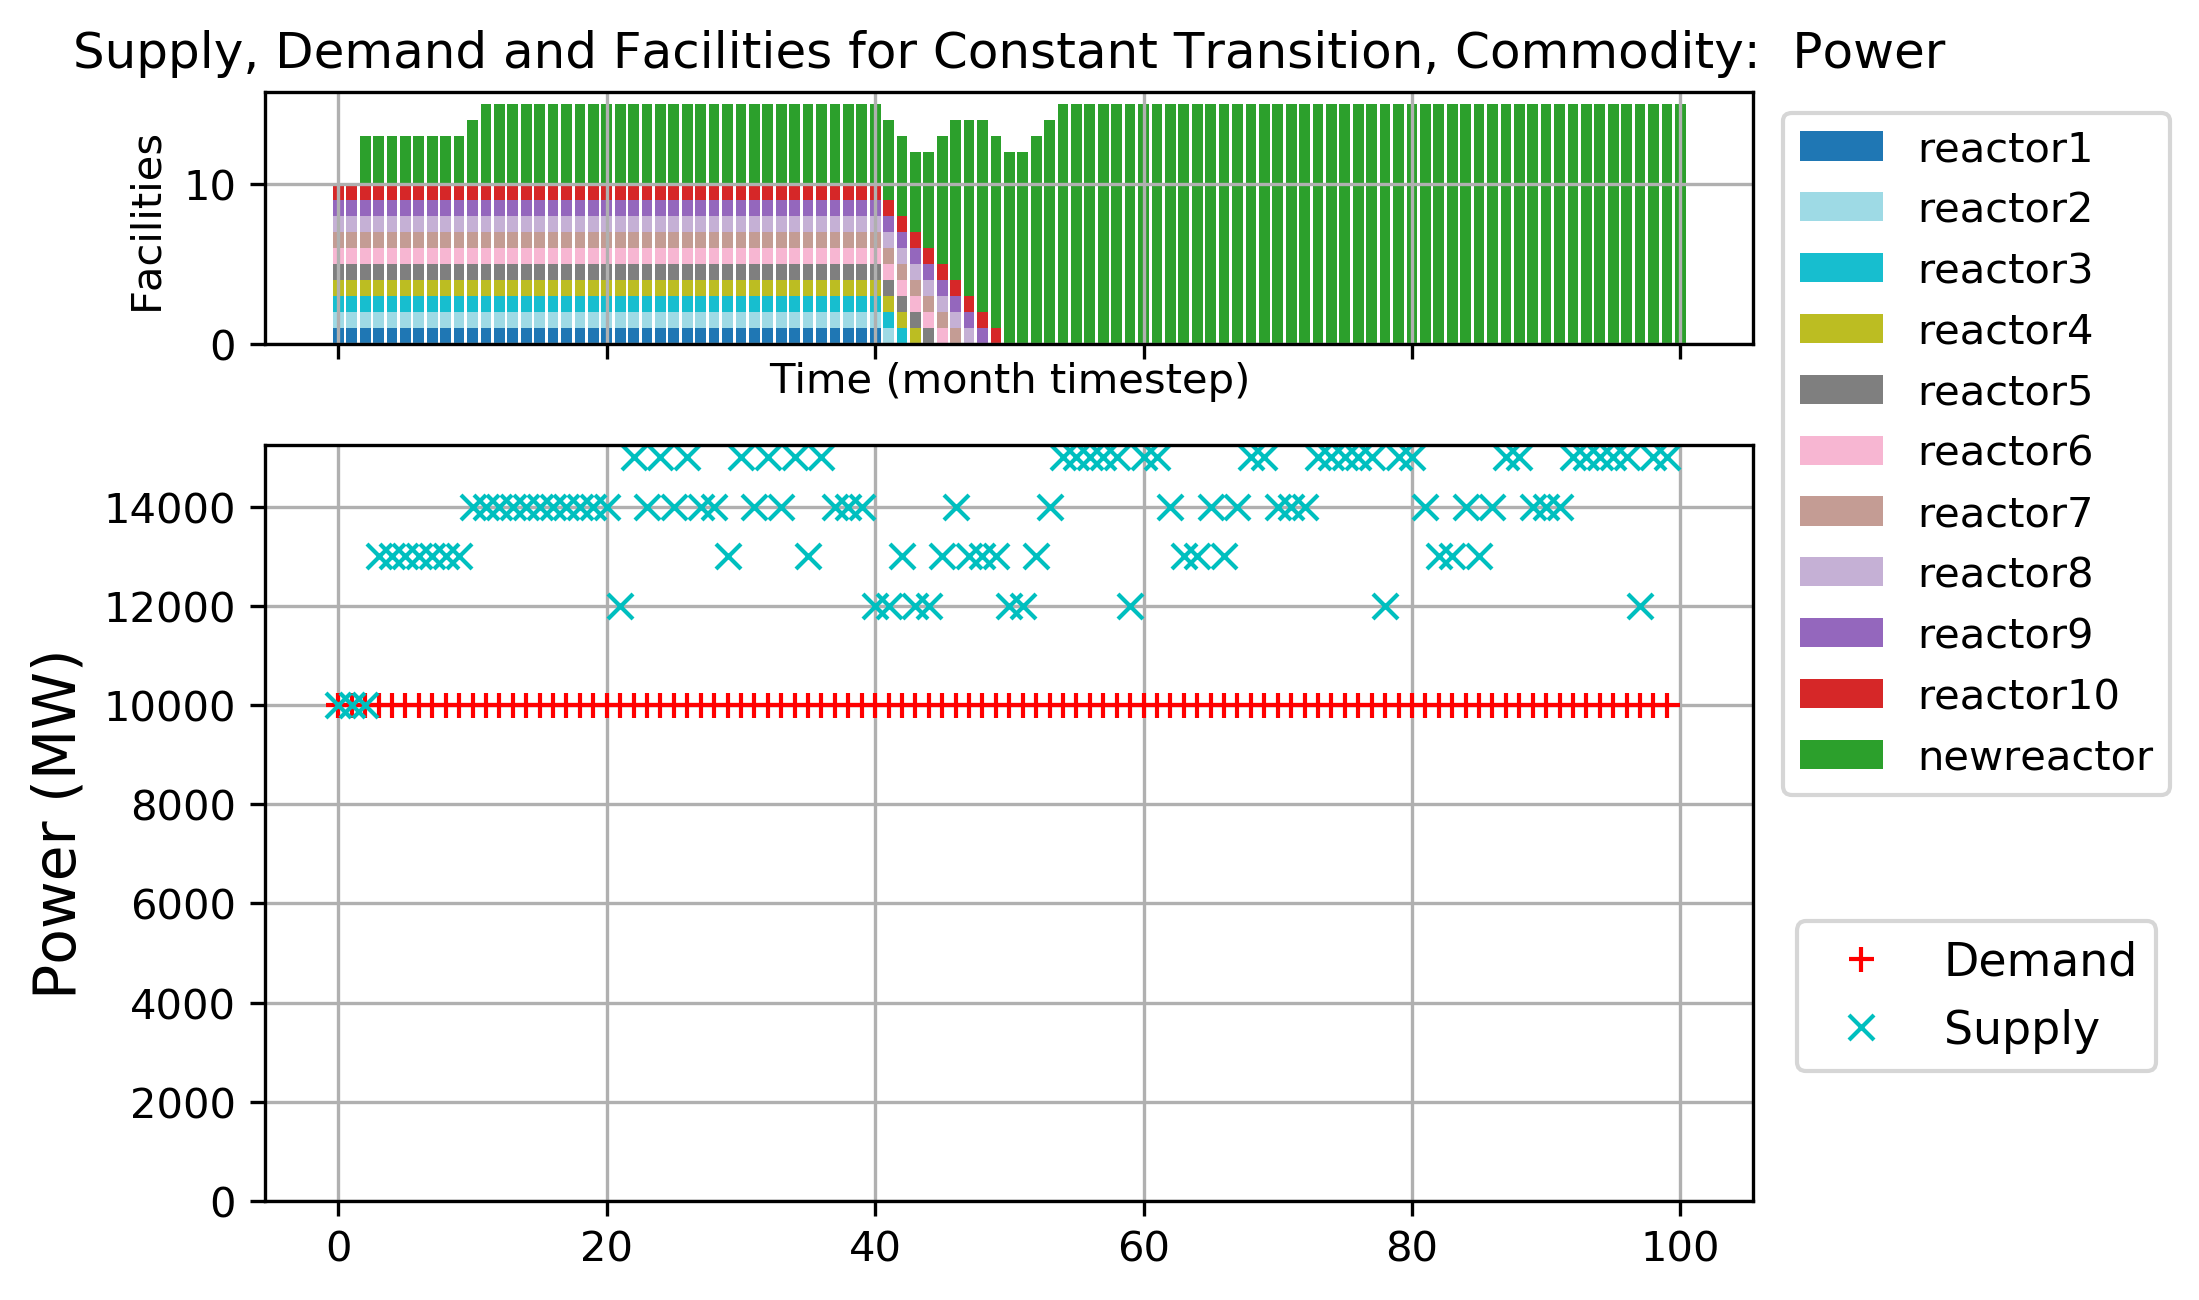
\includegraphics[width=\linewidth]{figures/constanttransition-power.png} 
        \caption{Power demand and supply plot.}
        \label{fig:constanttransition-power}
    \end{subfigure}
    \vspace{1cm}
    \begin{subfigure}[t]{0.45\textwidth}
        \centering
        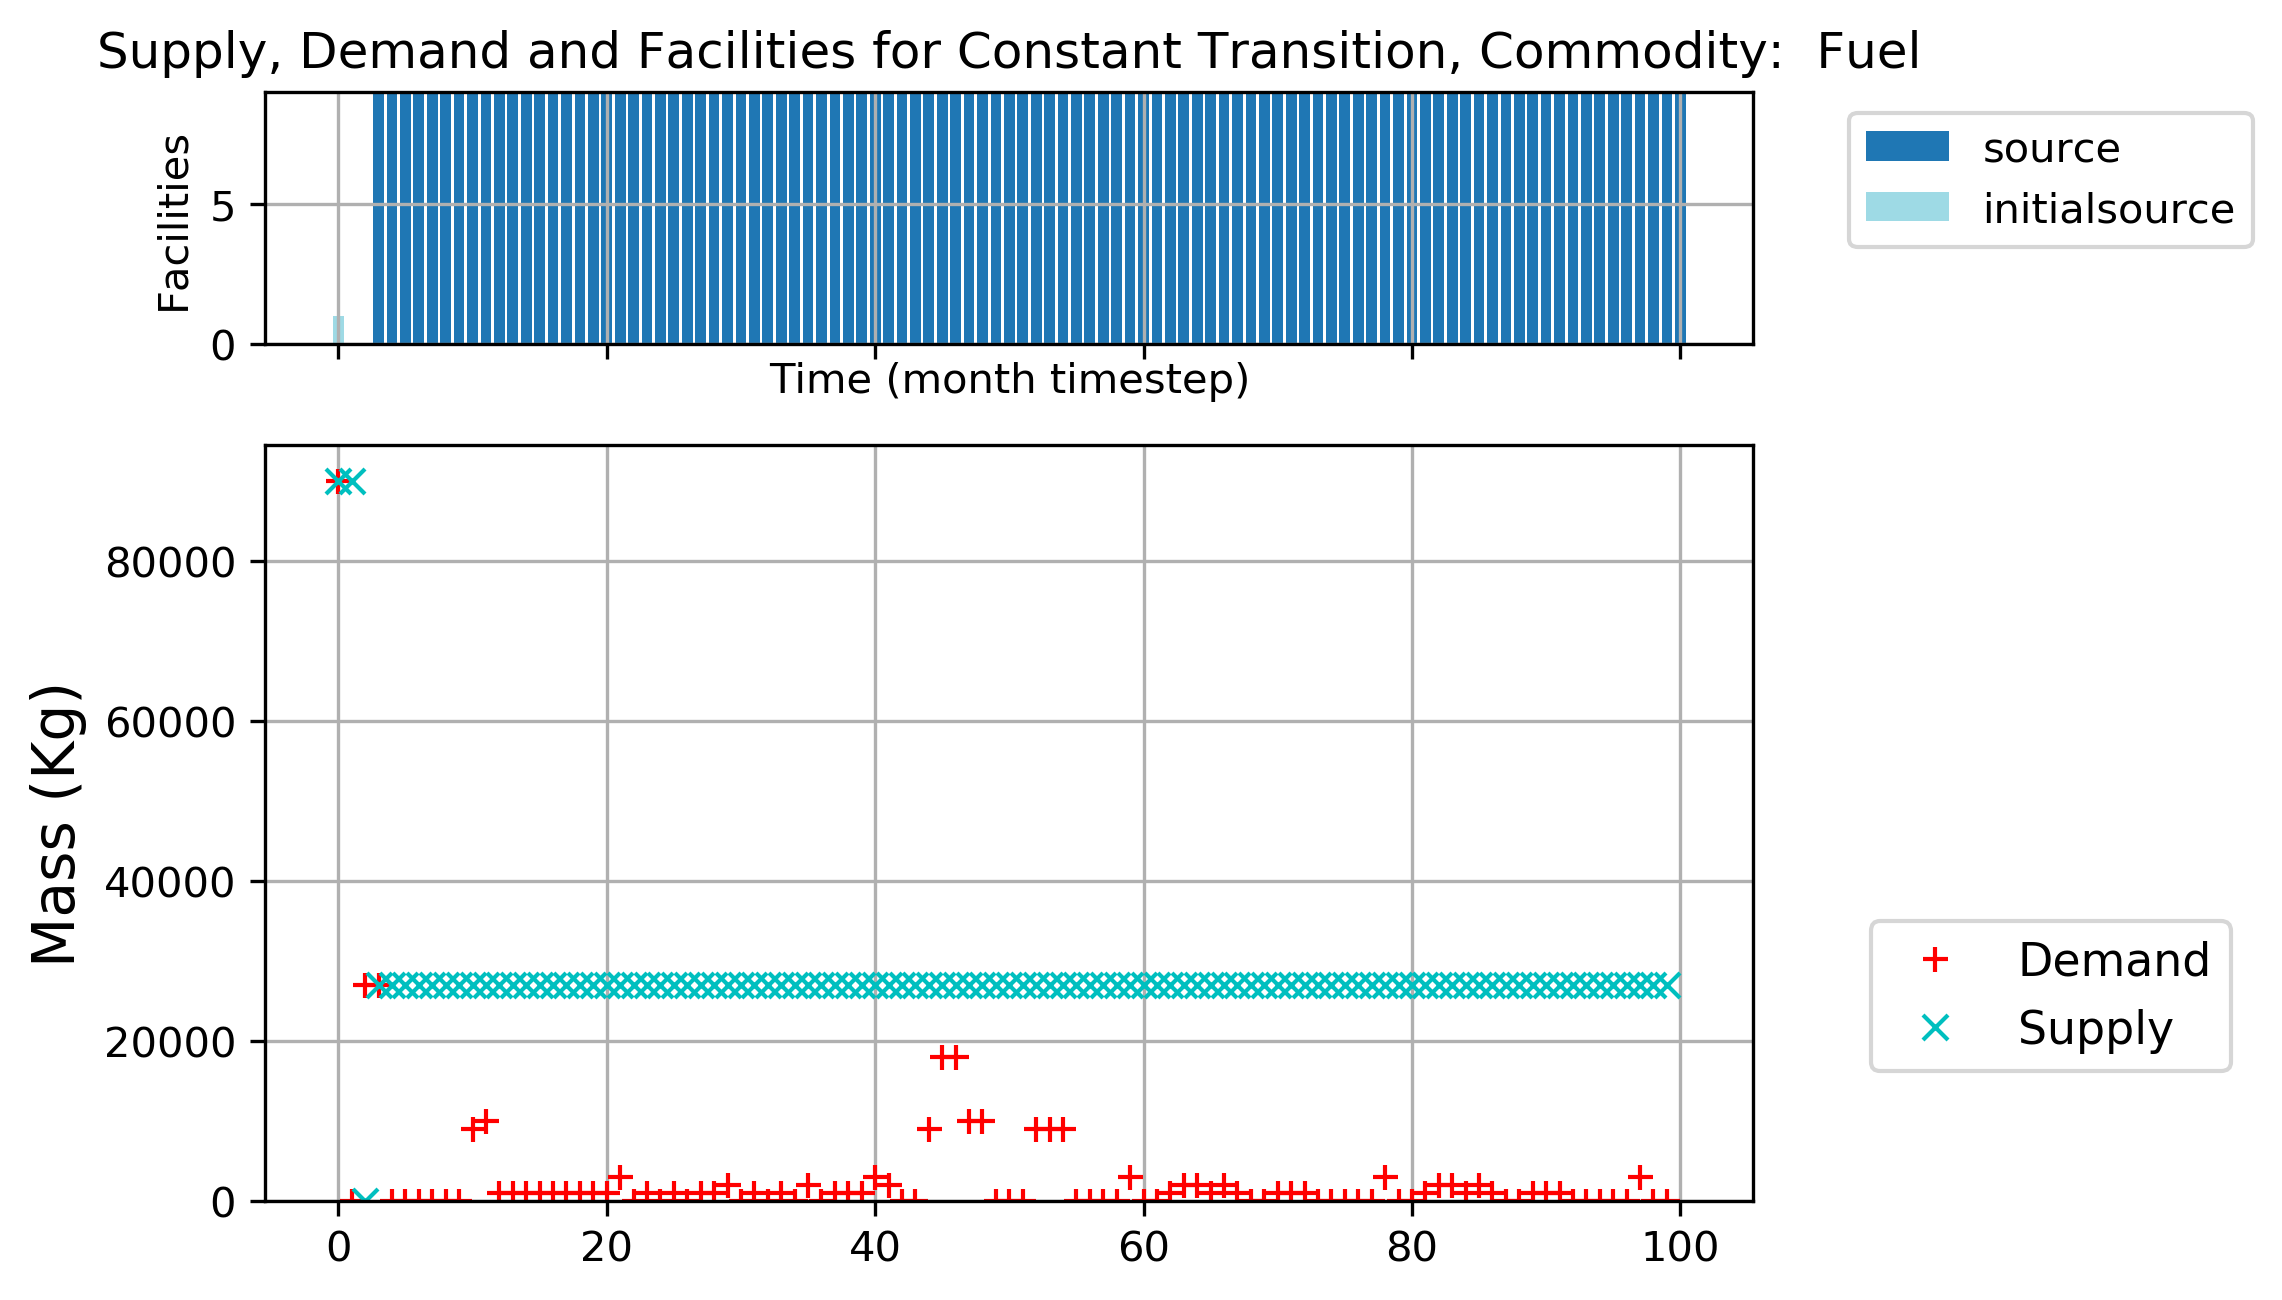
\includegraphics[width=\linewidth]{figures/constanttransition-fuel.png} 
        \caption{Fuel demand and supply plot.}
	    \label{fig:constanttransition-fuel}
    \end{subfigure}
    \hfill
    \begin{subfigure}[t]{0.45\textwidth}
        \centering
        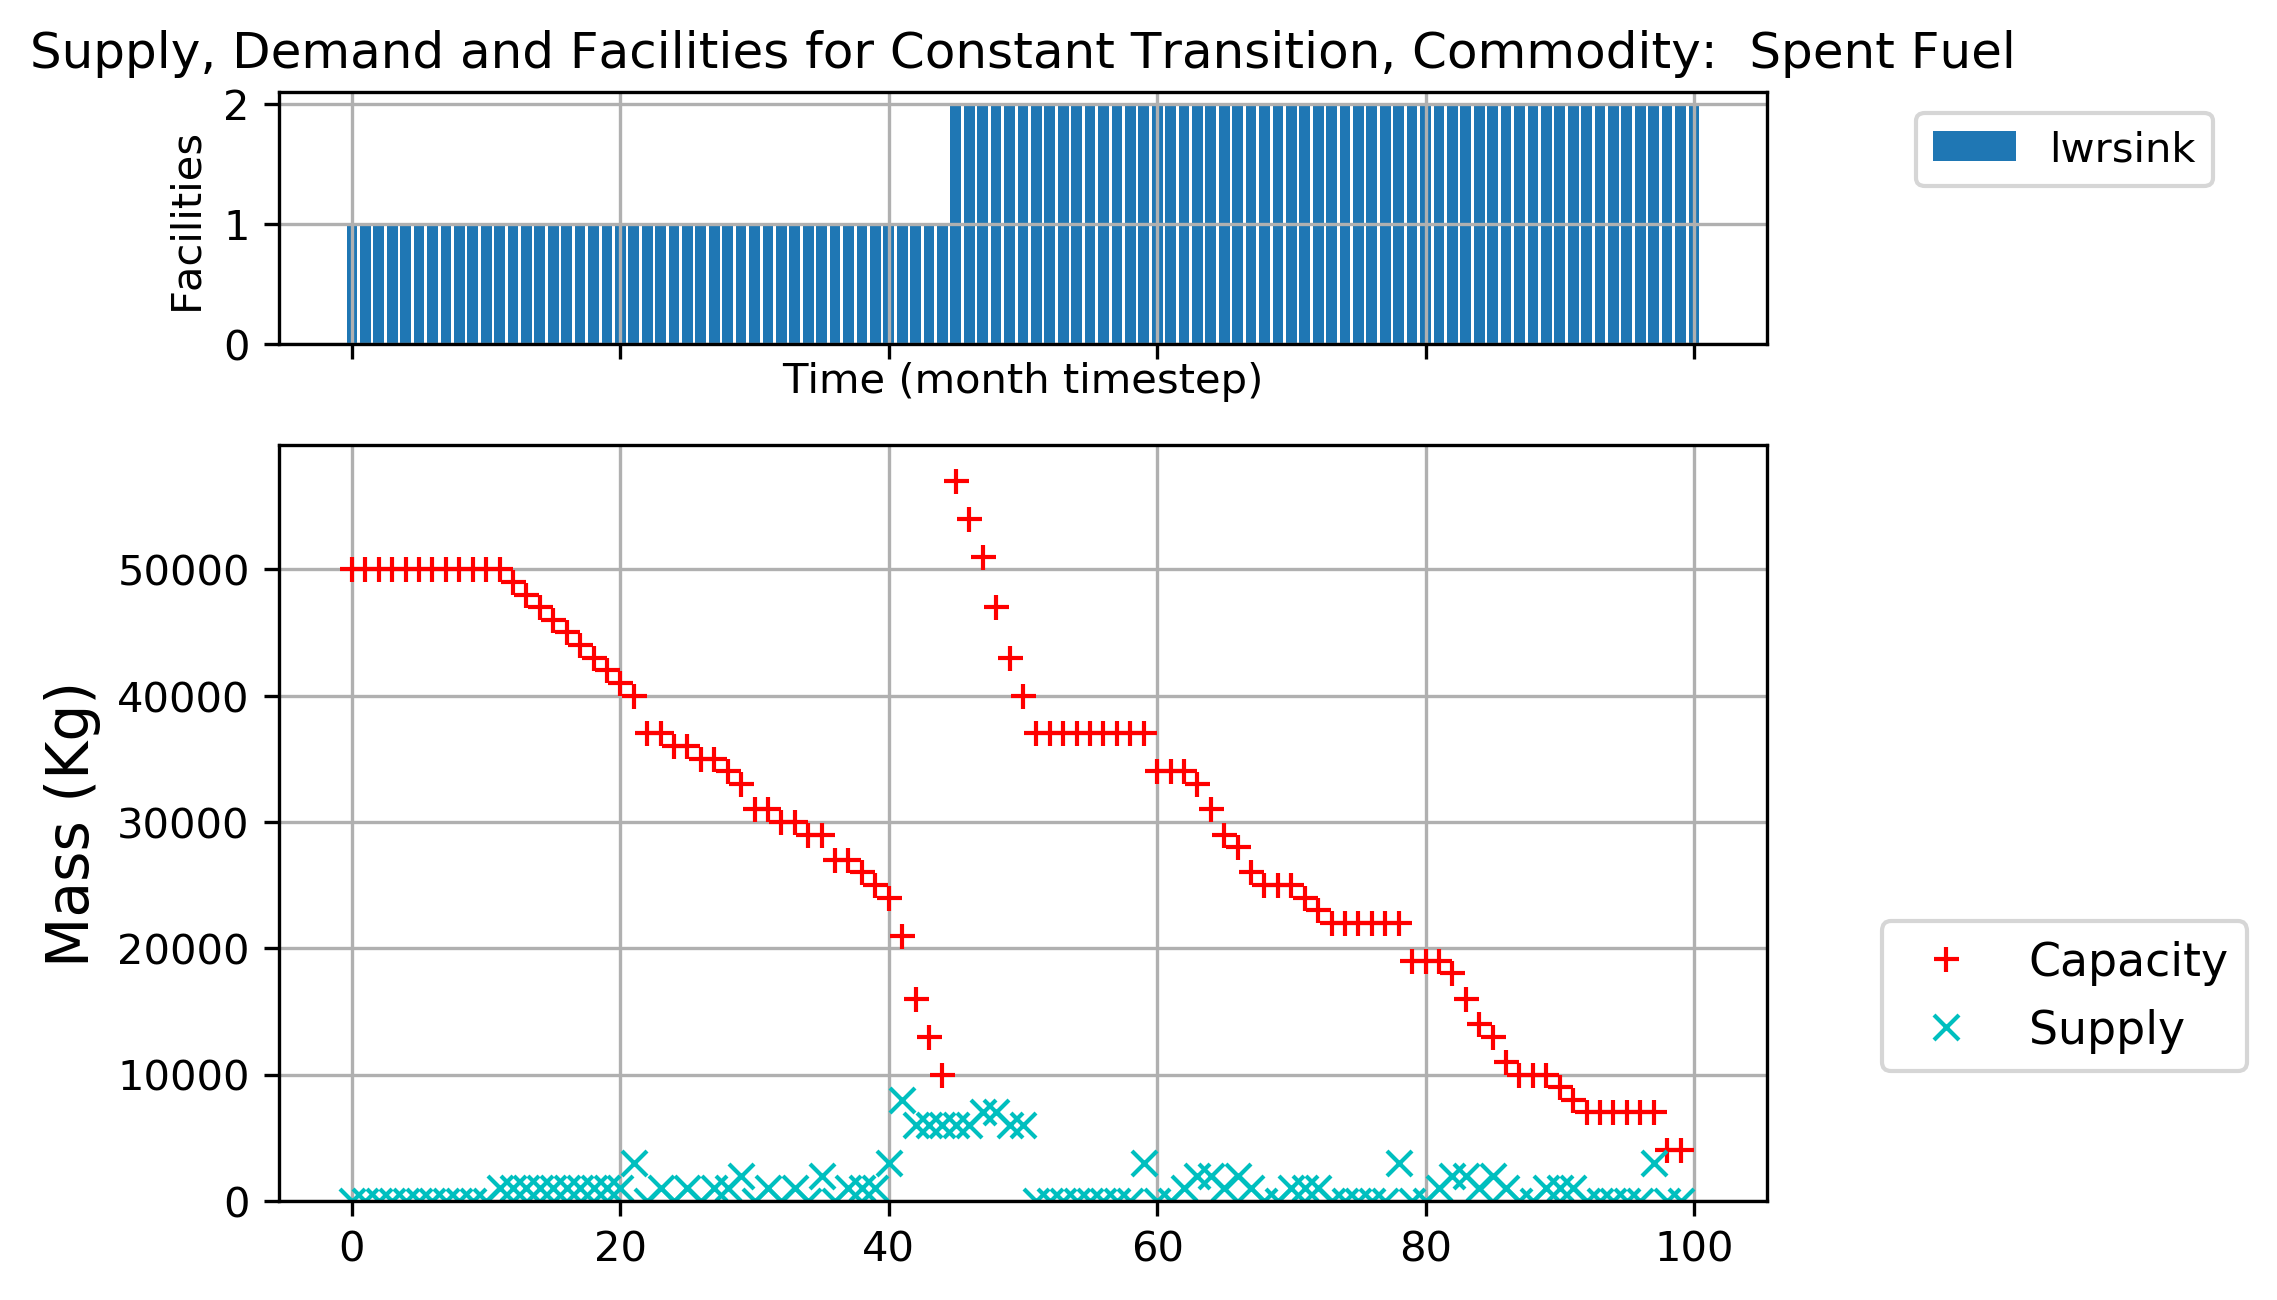
\includegraphics[width=\linewidth]{figures/constanttransition-spentfuel.png} 
        \caption{Spent Fuel demand and supply plot.}
        \label{fig:constanttransition-spentfuel}
    \end{subfigure}
    \caption{Transition Scenario: Constant Power Demand of 10000MW.}
\end{figure*}

\subsection{Transition Scenario: Linearly Increasing Demand}

This section presents a transition scenario with a linearly 
increasing power demand. 
Table \ref{tab:transition-scenario-growing-power} displays the 
simulation parameters used in this transition scenario. 

\begin{table*}[!htbp]
	\centering
	\caption {Linearly Increasing Power Demand Transition Scenario's Parameters.}
	\label{tab:transition-scenario-growing-power}
	\begin{tabular}{|l|l|p{4.1cm}|}
		\hline
		& \textbf{Parameters}    & \textbf{Description} \\ \hline
		\textbf{Overall}& Demand Equation & Time$<$40: 10000 MW, Time$>$40: 250*t MW \\ \hline
		\multirow{2}{*}{\textbf{Power Commodity}} & Prediction Method      &  Fast Fourier Transform \\ \cline{2-3} 
		& Supply Buffer          &  2000 MW \\ \hline
		\multirow{2}{*}{\textbf{Fuel Commodity}}  & Prediction Method      &  Moving Average\\ \cline{2-3}
		& Supply Buffer & 1000 kg \\ \hline
		\multirow{2}{*}{\textbf{Spent Fuel Commodity}}  & Prediction Method      &  Fast Fourier Transform \\ \cline{2-3}
		& Capacity Buffer & 0 kg \\ \hline
	\end{tabular}
\end{table*}

Figures \ref{fig:growingtransition-power}, \ref{fig:growingtransition-fuel}
and \ref{fig:growingtransition-spentfuel} demonstrate the capability 
of \deploy to deploy reactors and supporting facilities to meet the user 
determined power demand and subsequently required secondary commodities 
for a linearly increasing power demand. 

This scenario made use of the fast fourier transform method for predicting power
demand, similar to what the constant power demand transition scenario used.
The power supply buffer in this case was an absolute value of 2000MW. 

The input file used to generate this simulation can be found in:

\noindent
$/d3ploy/input/growing\_transition.xml$

\noindent
and the file used to run the simulation and generate the plots can be found in:

\noindent
$/d3ploy/tests/performance\_tests/algorithm\_performance\_tests\_transitions.py$

\begin{figure*}[!htbp]
    \centering
    \begin{subfigure}[t]{\textwidth}
    \centering
        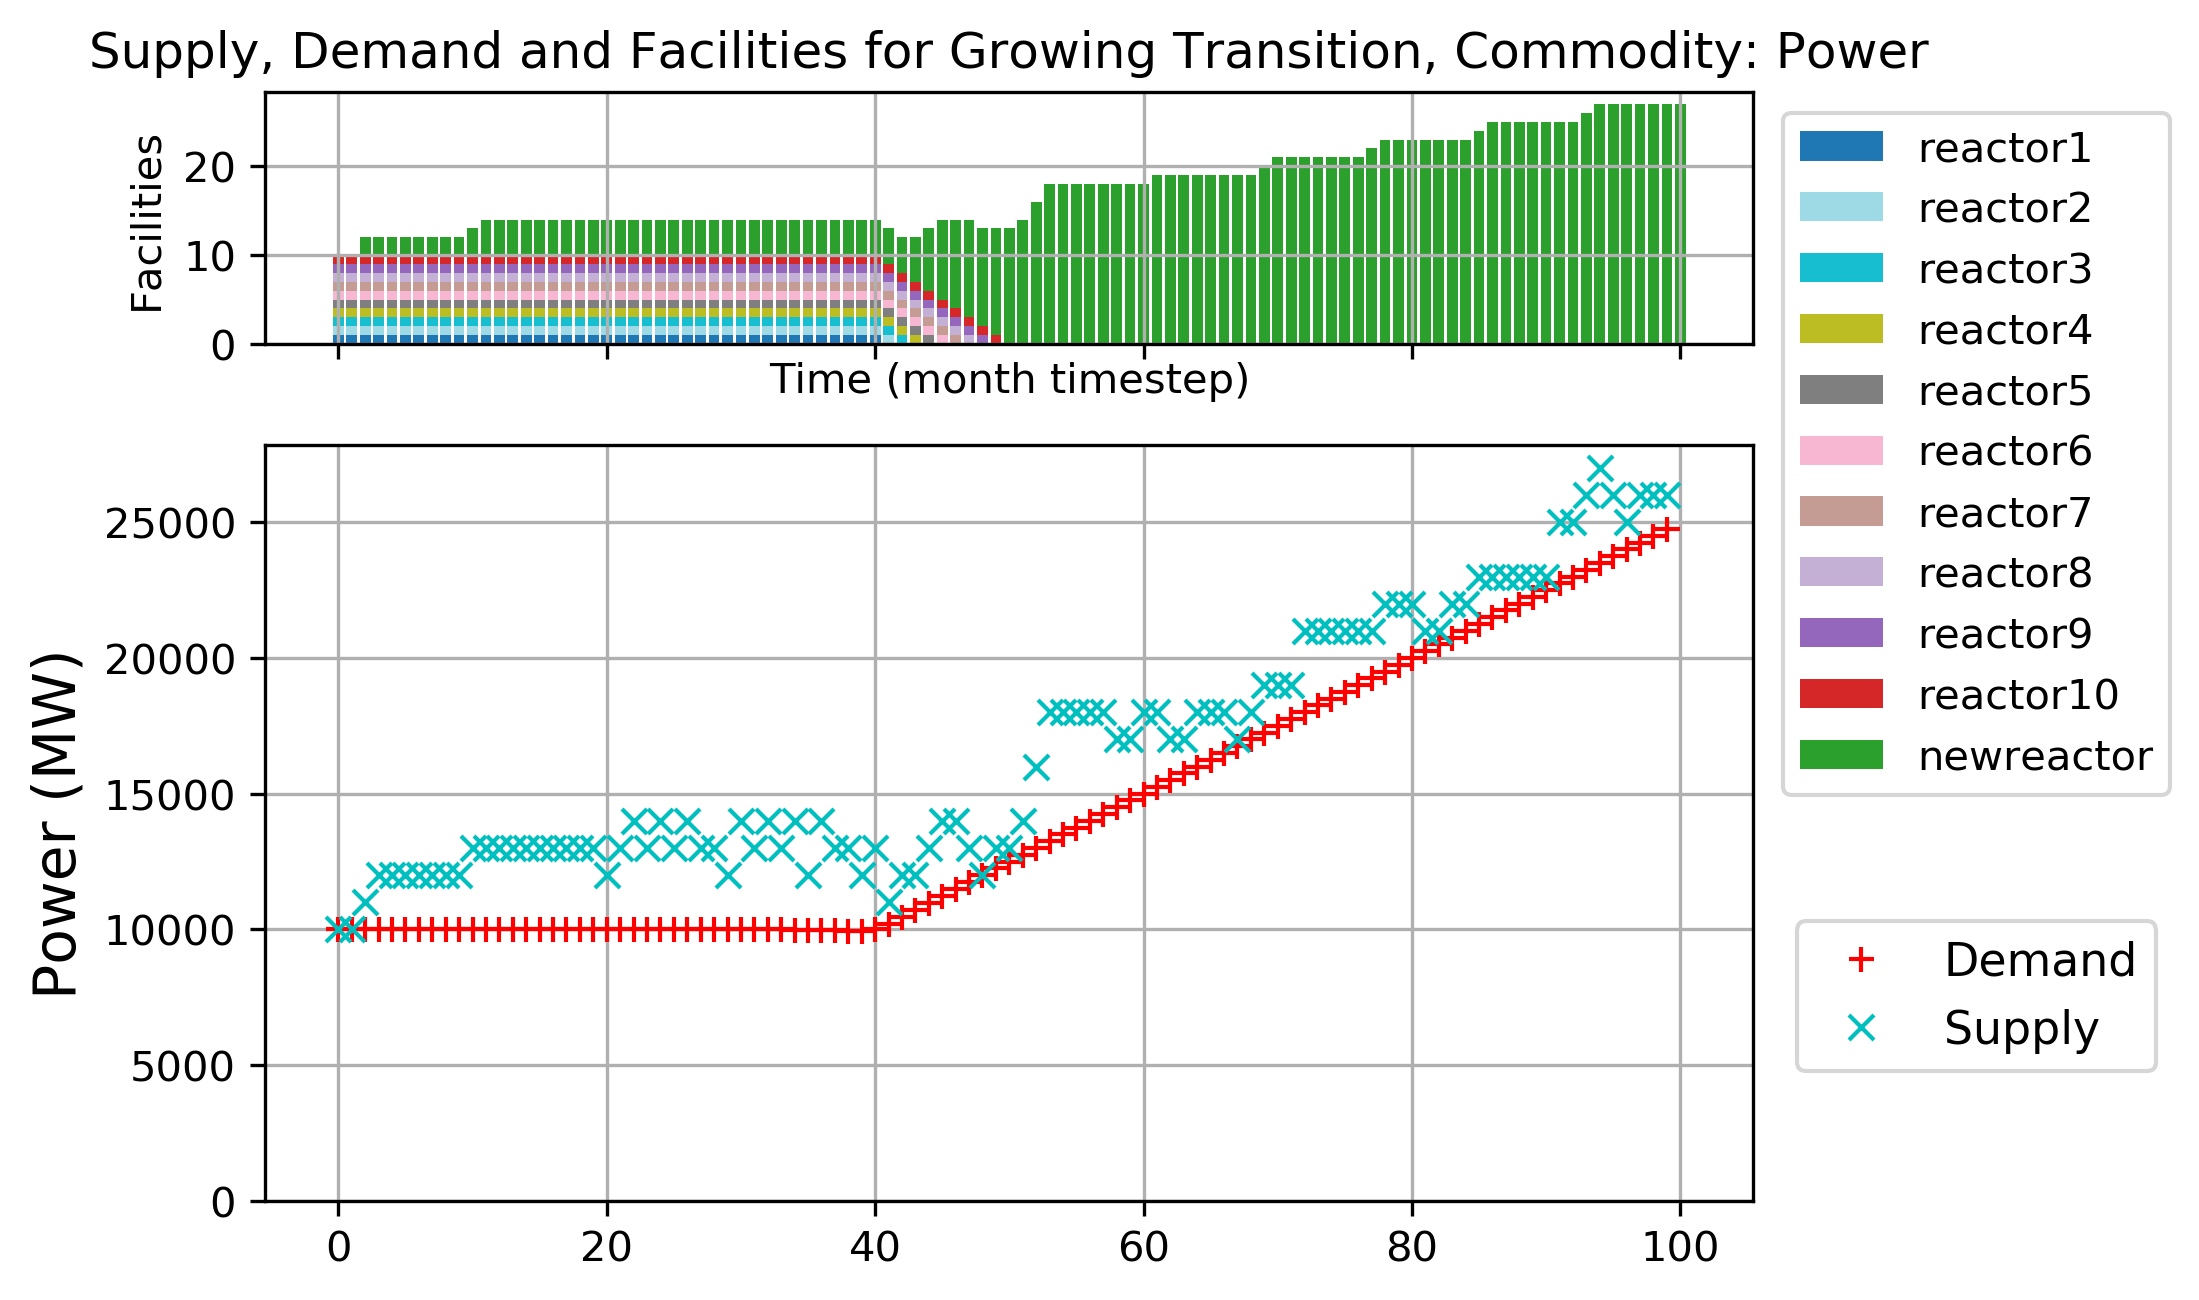
\includegraphics[width=\linewidth]{figures/growingtransition-power.png} 
        \caption{Power demand and supply plot.}
        \label{fig:growingtransition-power}
    \end{subfigure}
    \vspace{1cm}
    \begin{subfigure}[t]{0.45\textwidth}
        \centering
        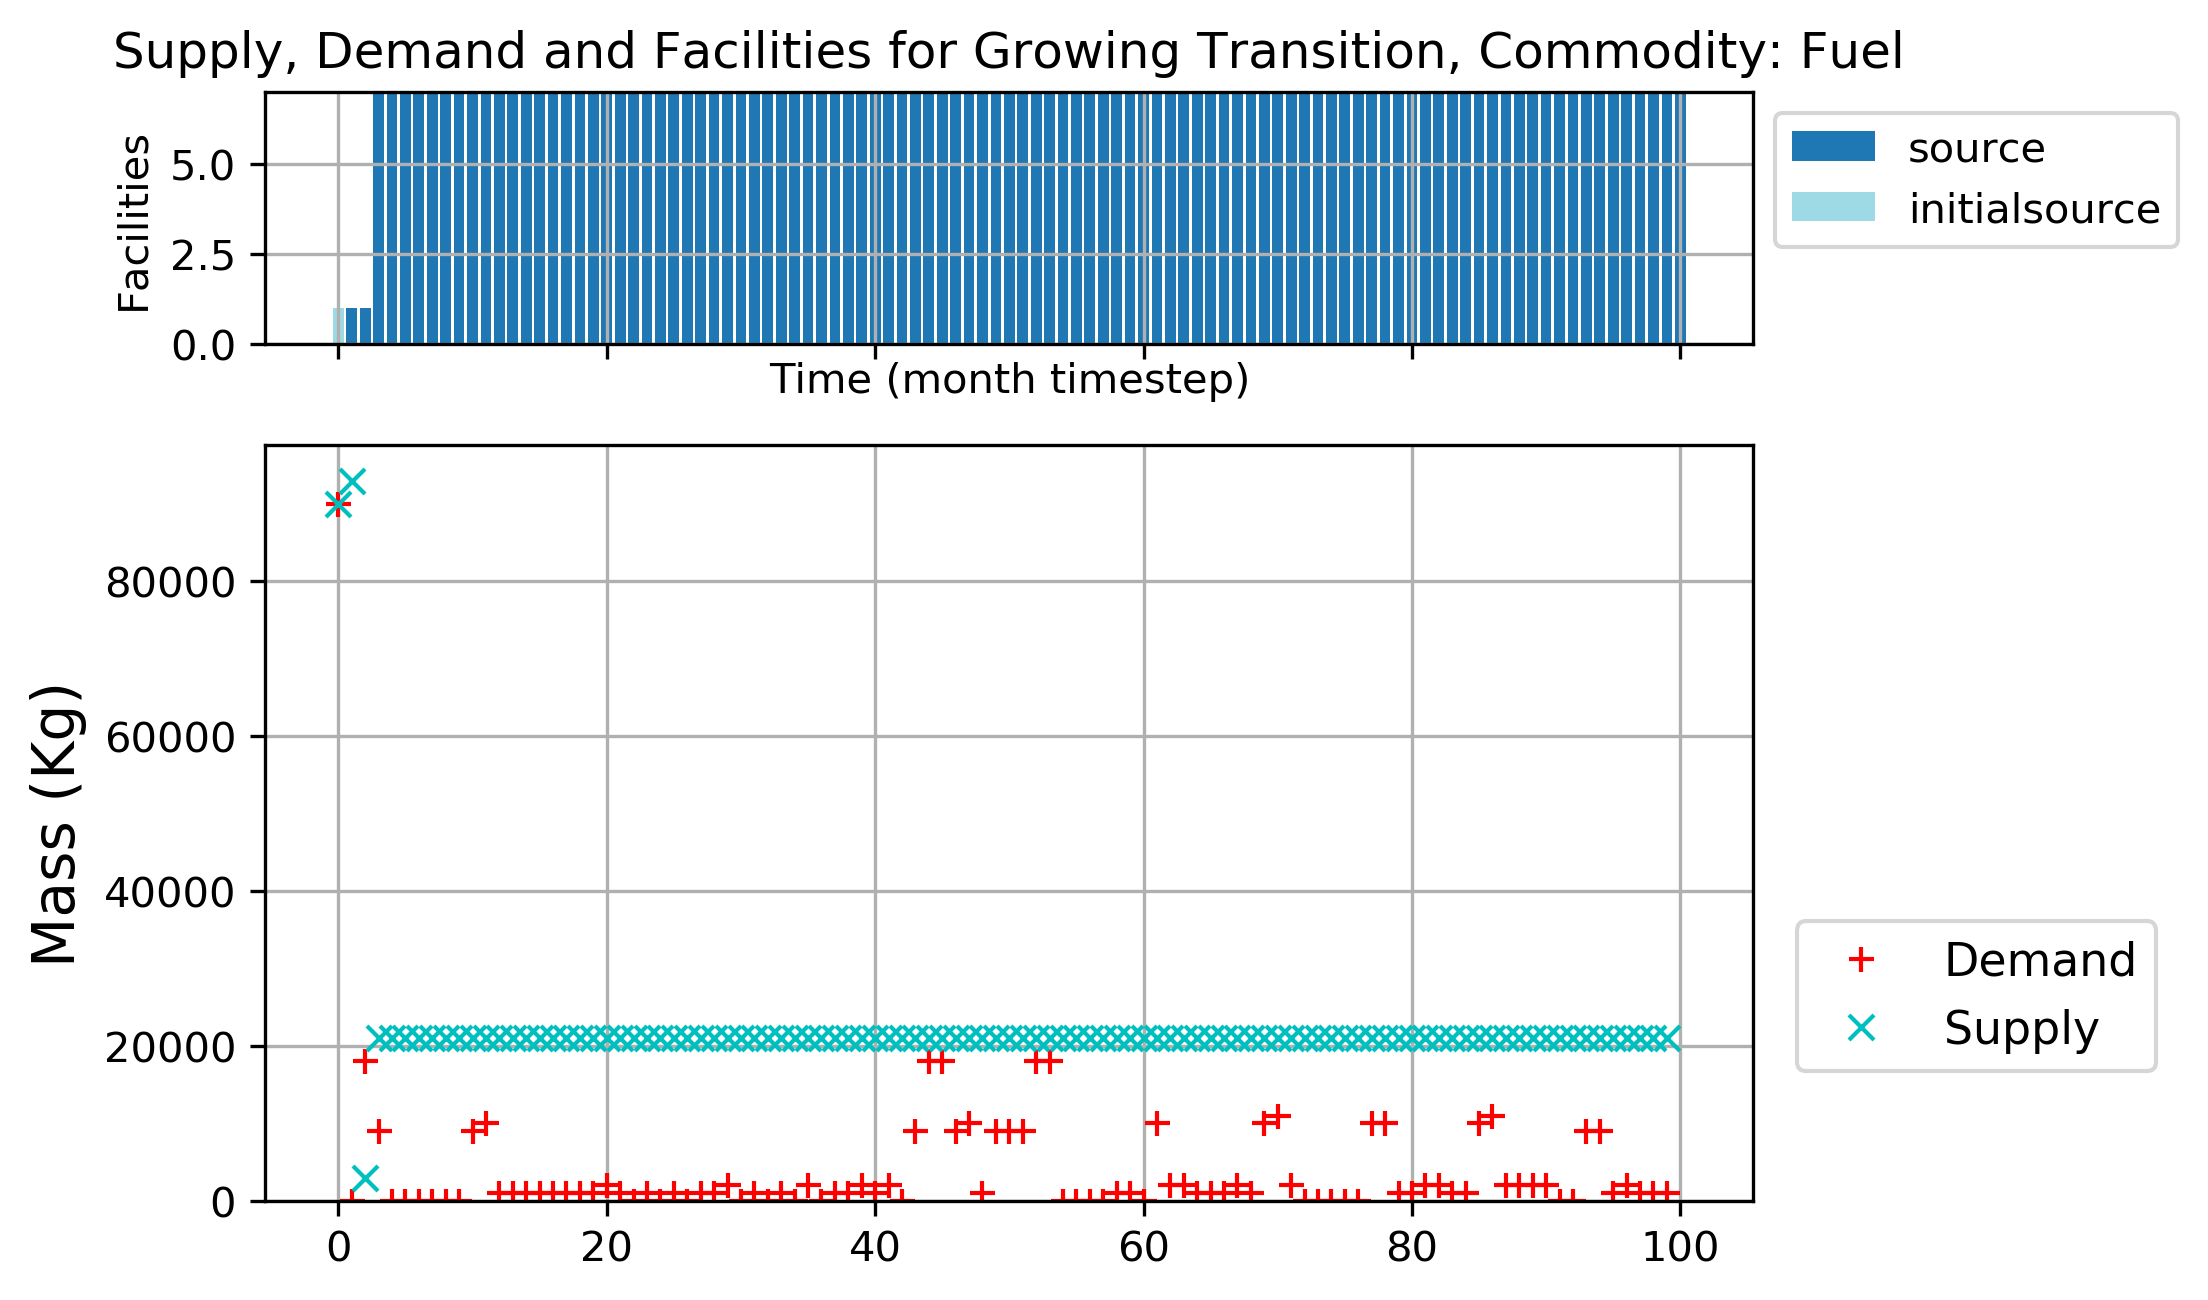
\includegraphics[width=\linewidth]{figures/growingtransition-fuel.png} 
        \caption{Fuel demand and supply plot.}
	    \label{fig:growingtransition-fuel}
    \end{subfigure}
    \hfill
    \begin{subfigure}[t]{0.45\textwidth}
        \centering
        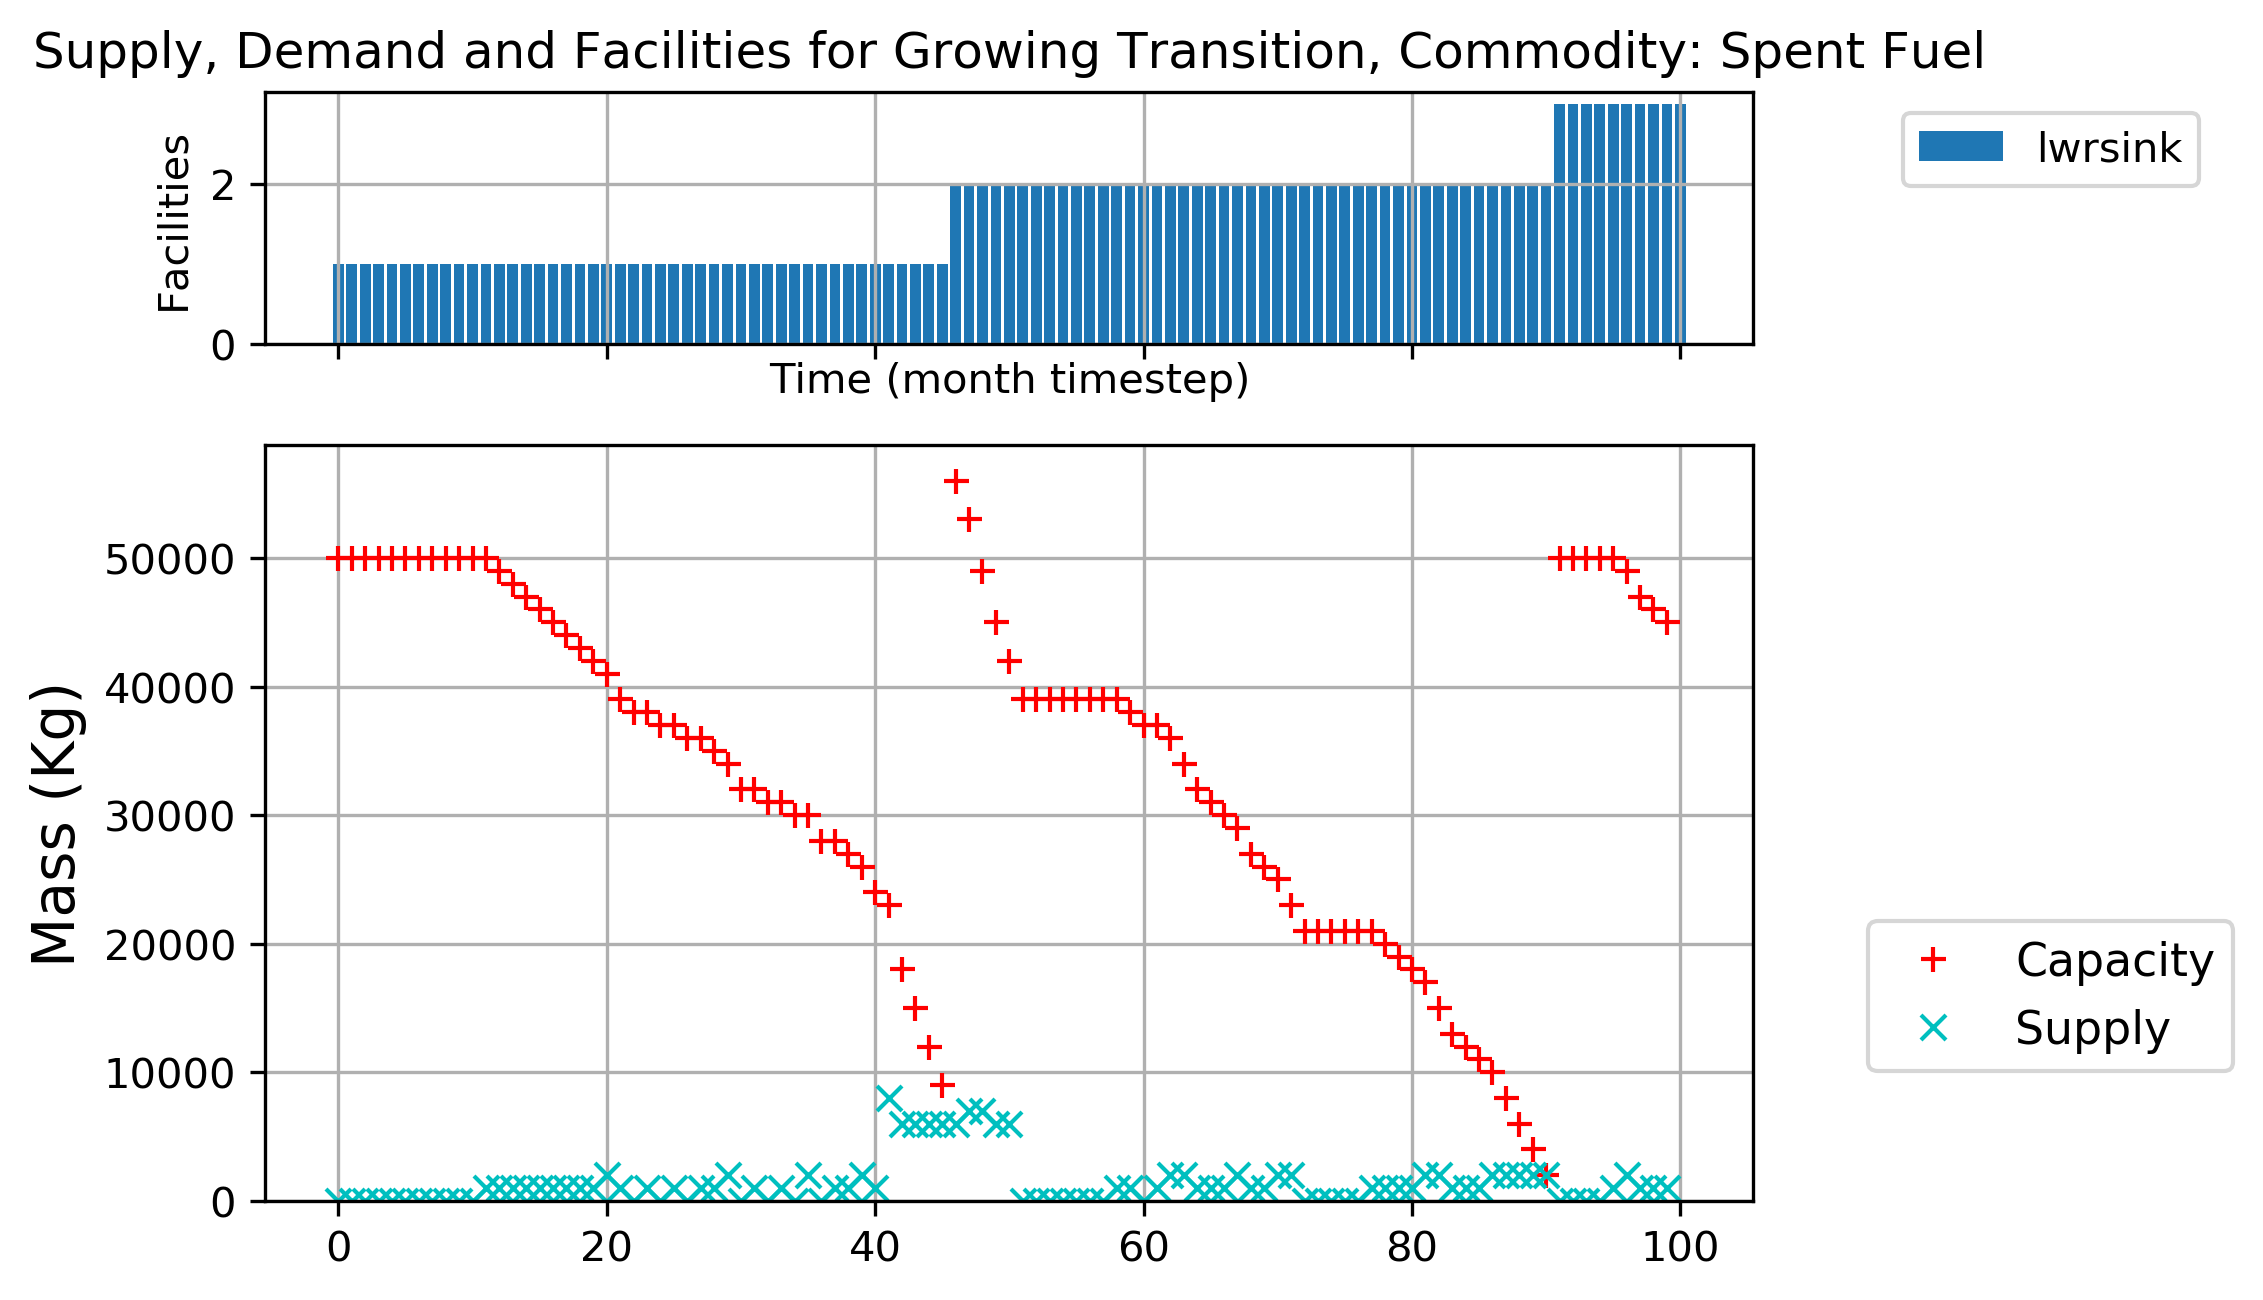
\includegraphics[width=\linewidth]{figures/growingtransition-spentfuel.png} 
        \caption{Spent Fuel demand and supply plot.}
        \label{fig:growingtransition-spentfuel}
    \end{subfigure}
    \caption{Transition Scenario: Linearly Increasing Power Demand.}
\end{figure*}

\subsection{\textbf{Transition Scenario: Sinusoidal Demand}}
This section shows a transition scenario with sinusoidal
power demand. 
A sinusoidal power demand is a more accurate reflection of
the real world where consumption is higher in the winter and summer
and lower in the spring and fall. 
Table \ref{tab:transition-scenario-sine-power} displays the 
simulation parameters used in this transition scenario. The power demand
had an amplitude of 1000MW.

Figures \ref{fig:sinetransition-power}, \ref{fig:sinetransition-fuel}
and \ref{fig:sinetransition-spentfuel} demonstrate the capability 
of \deploy to deploy reactors and supporting facilities to meet the user 
determined power demand and subsequently required secondary commodities 
for a sinusoidal power demand. 

For a sinusoidal power demand, the use of the triple exponential method
(Holt-Winters)
for predicting demand is more effective than the 
fast fourier transform method previously used in the constant 
and linearly increasing power demand transition scenarios. 
This is because the triple exponential smoothing method excels in
forecasting data points for repetitive seasonal series of data.  

\begin{table*}[!htbp]
	\centering
	\caption {Sinusoidal Power Demand Transition Scenario's Parameters.}
	\label{tab:transition-scenario-sine-power}
	\begin{tabular}{|l|l|p{4.5cm}|}
		\hline
		& \textbf{Parameters}    & \textbf{Description} \\ \hline
		\textbf{Overall}& Demand Equation & $1000sin(\frac{\pi*t}{3})+10000$ \\ \hline
		\multirow{2}{*}{\textbf{Power Commodity}} & Prediction Method      &  Triple Exponential Smoothing \\ \cline{2-3} 
		& Supply Buffer          &  2000 MW \\ \hline
		\multirow{2}{*}{\textbf{Fuel Commodity}}  & Prediction Method      &  Moving Average\\ \cline{2-3}
		& Supply Buffer & 1000 kg \\ \hline
		\multirow{2}{*}{\textbf{Spent Fuel Commodity}}  & Prediction Method      & Fast Fourier Transform\\ \cline{2-3}
		& Capacity Buffer & 0 kg \\ \hline
	\end{tabular}
\end{table*}

The input file used to generate this simulation can be found in:

\noindent
$/d3ploy/input/sine\_transition.xml$

\noindent
and the file used to run the simulation and generate the plots can be found in:

\noindent
$/d3ploy/tests/performance\_tests/algorithm\_performance\_tests\_transitions.py$

\begin{figure*}[!htbp]
    \centering
    \begin{subfigure}[t]{\textwidth}
    \centering
        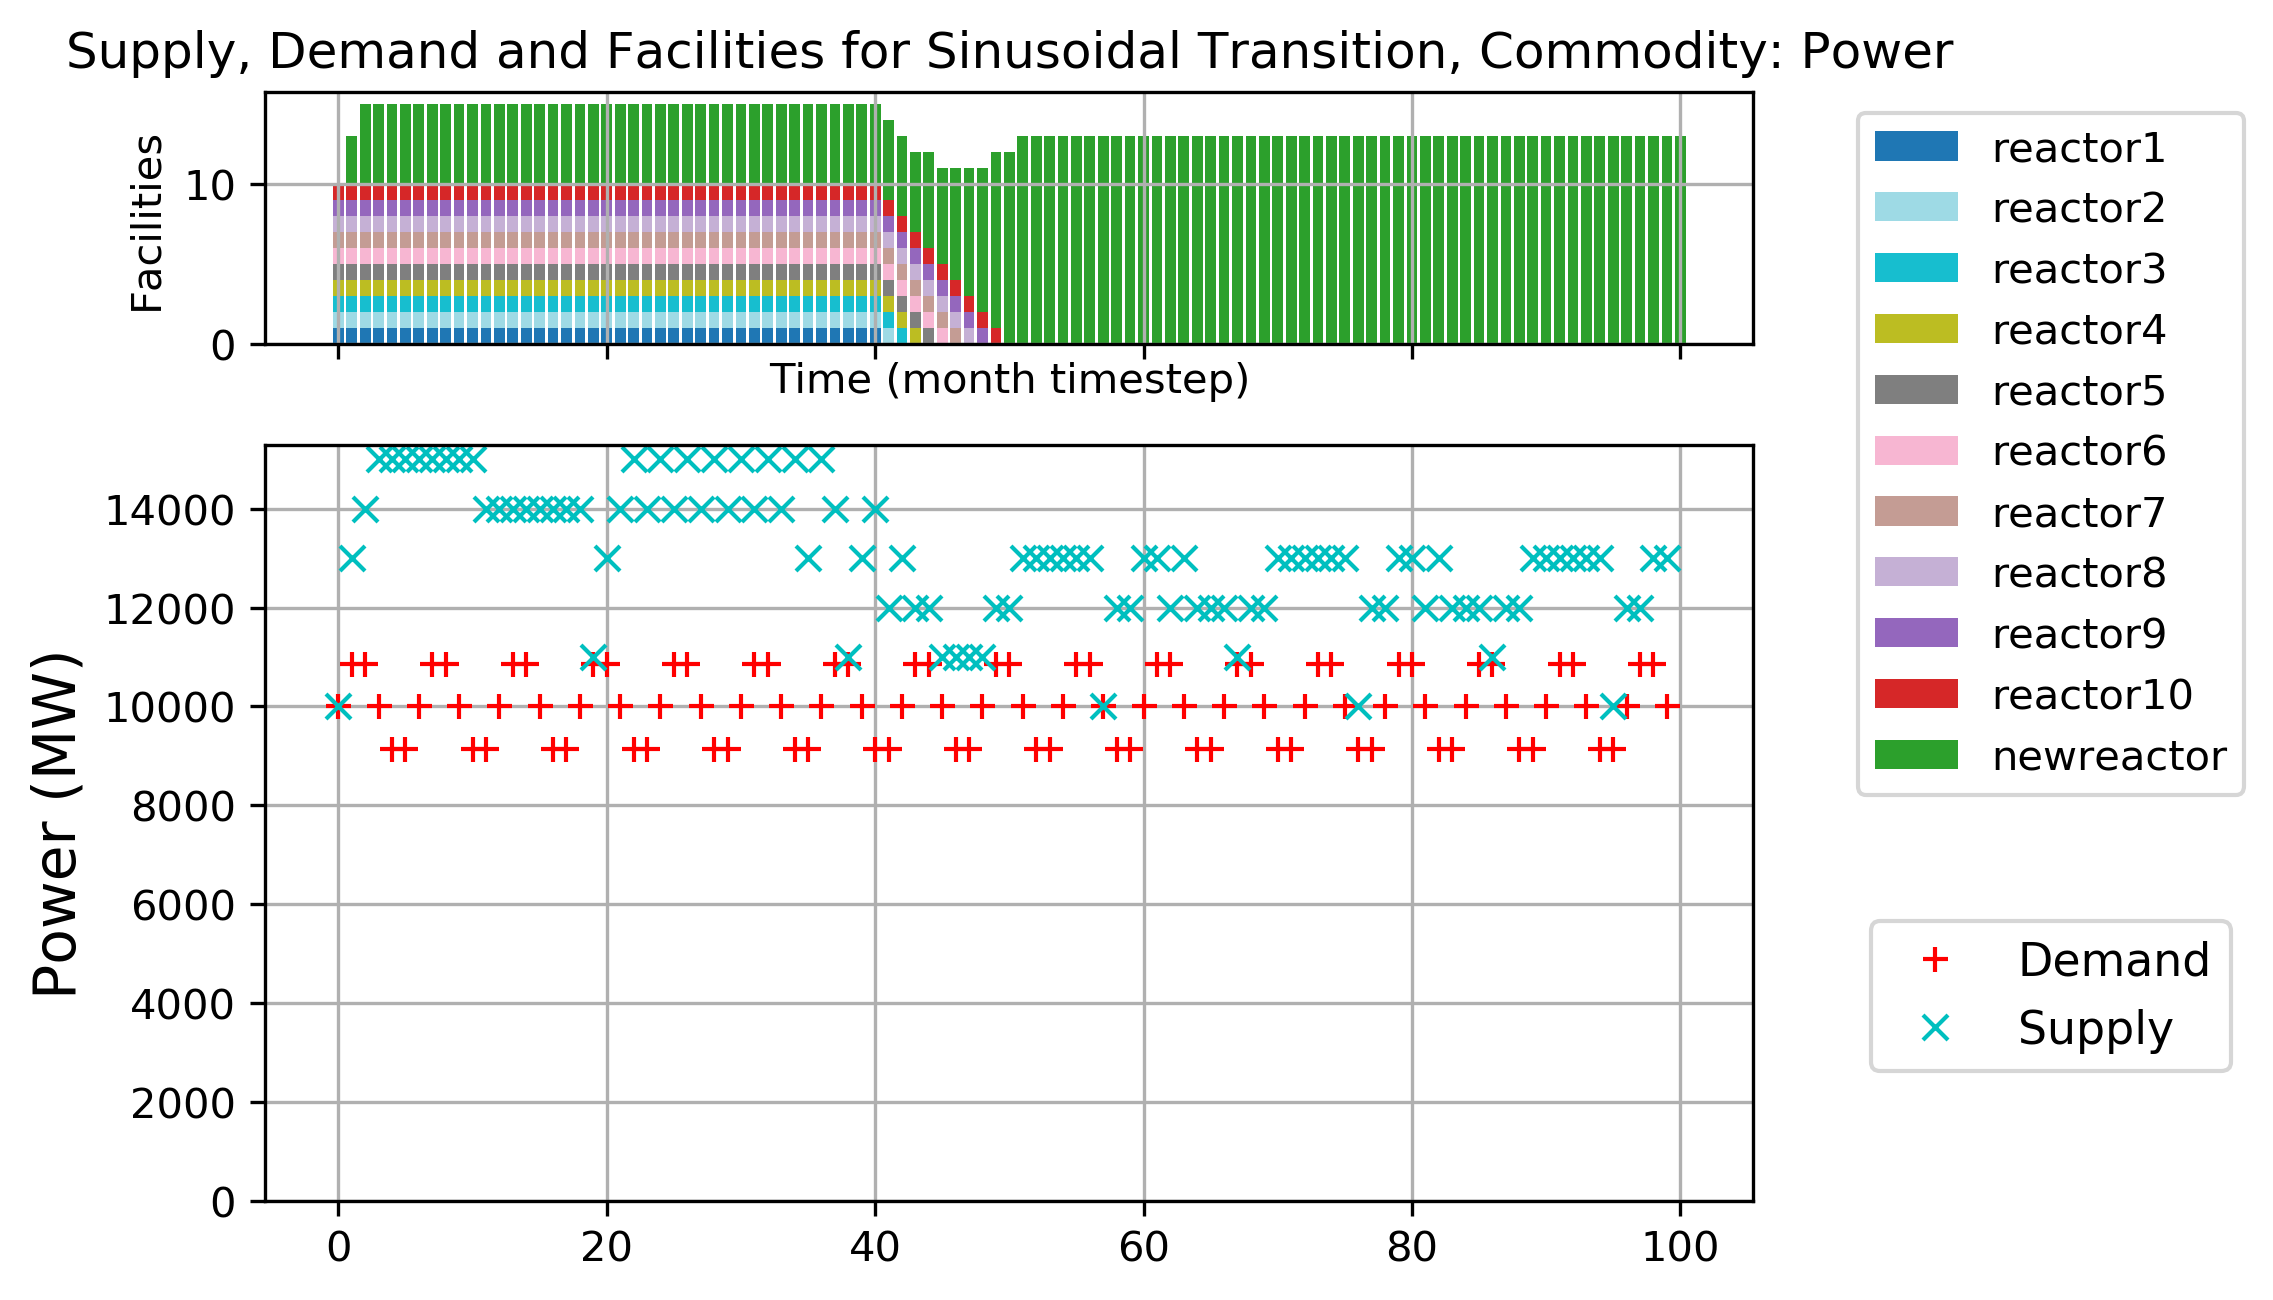
\includegraphics[width=\linewidth]{figures/sinetransition-power.png} 
        \caption{Power demand and supply plot.}
        \label{fig:sinetransition-power}
    \end{subfigure}
    \vspace{1cm}
    \begin{subfigure}[t]{0.45\textwidth}
        \centering
        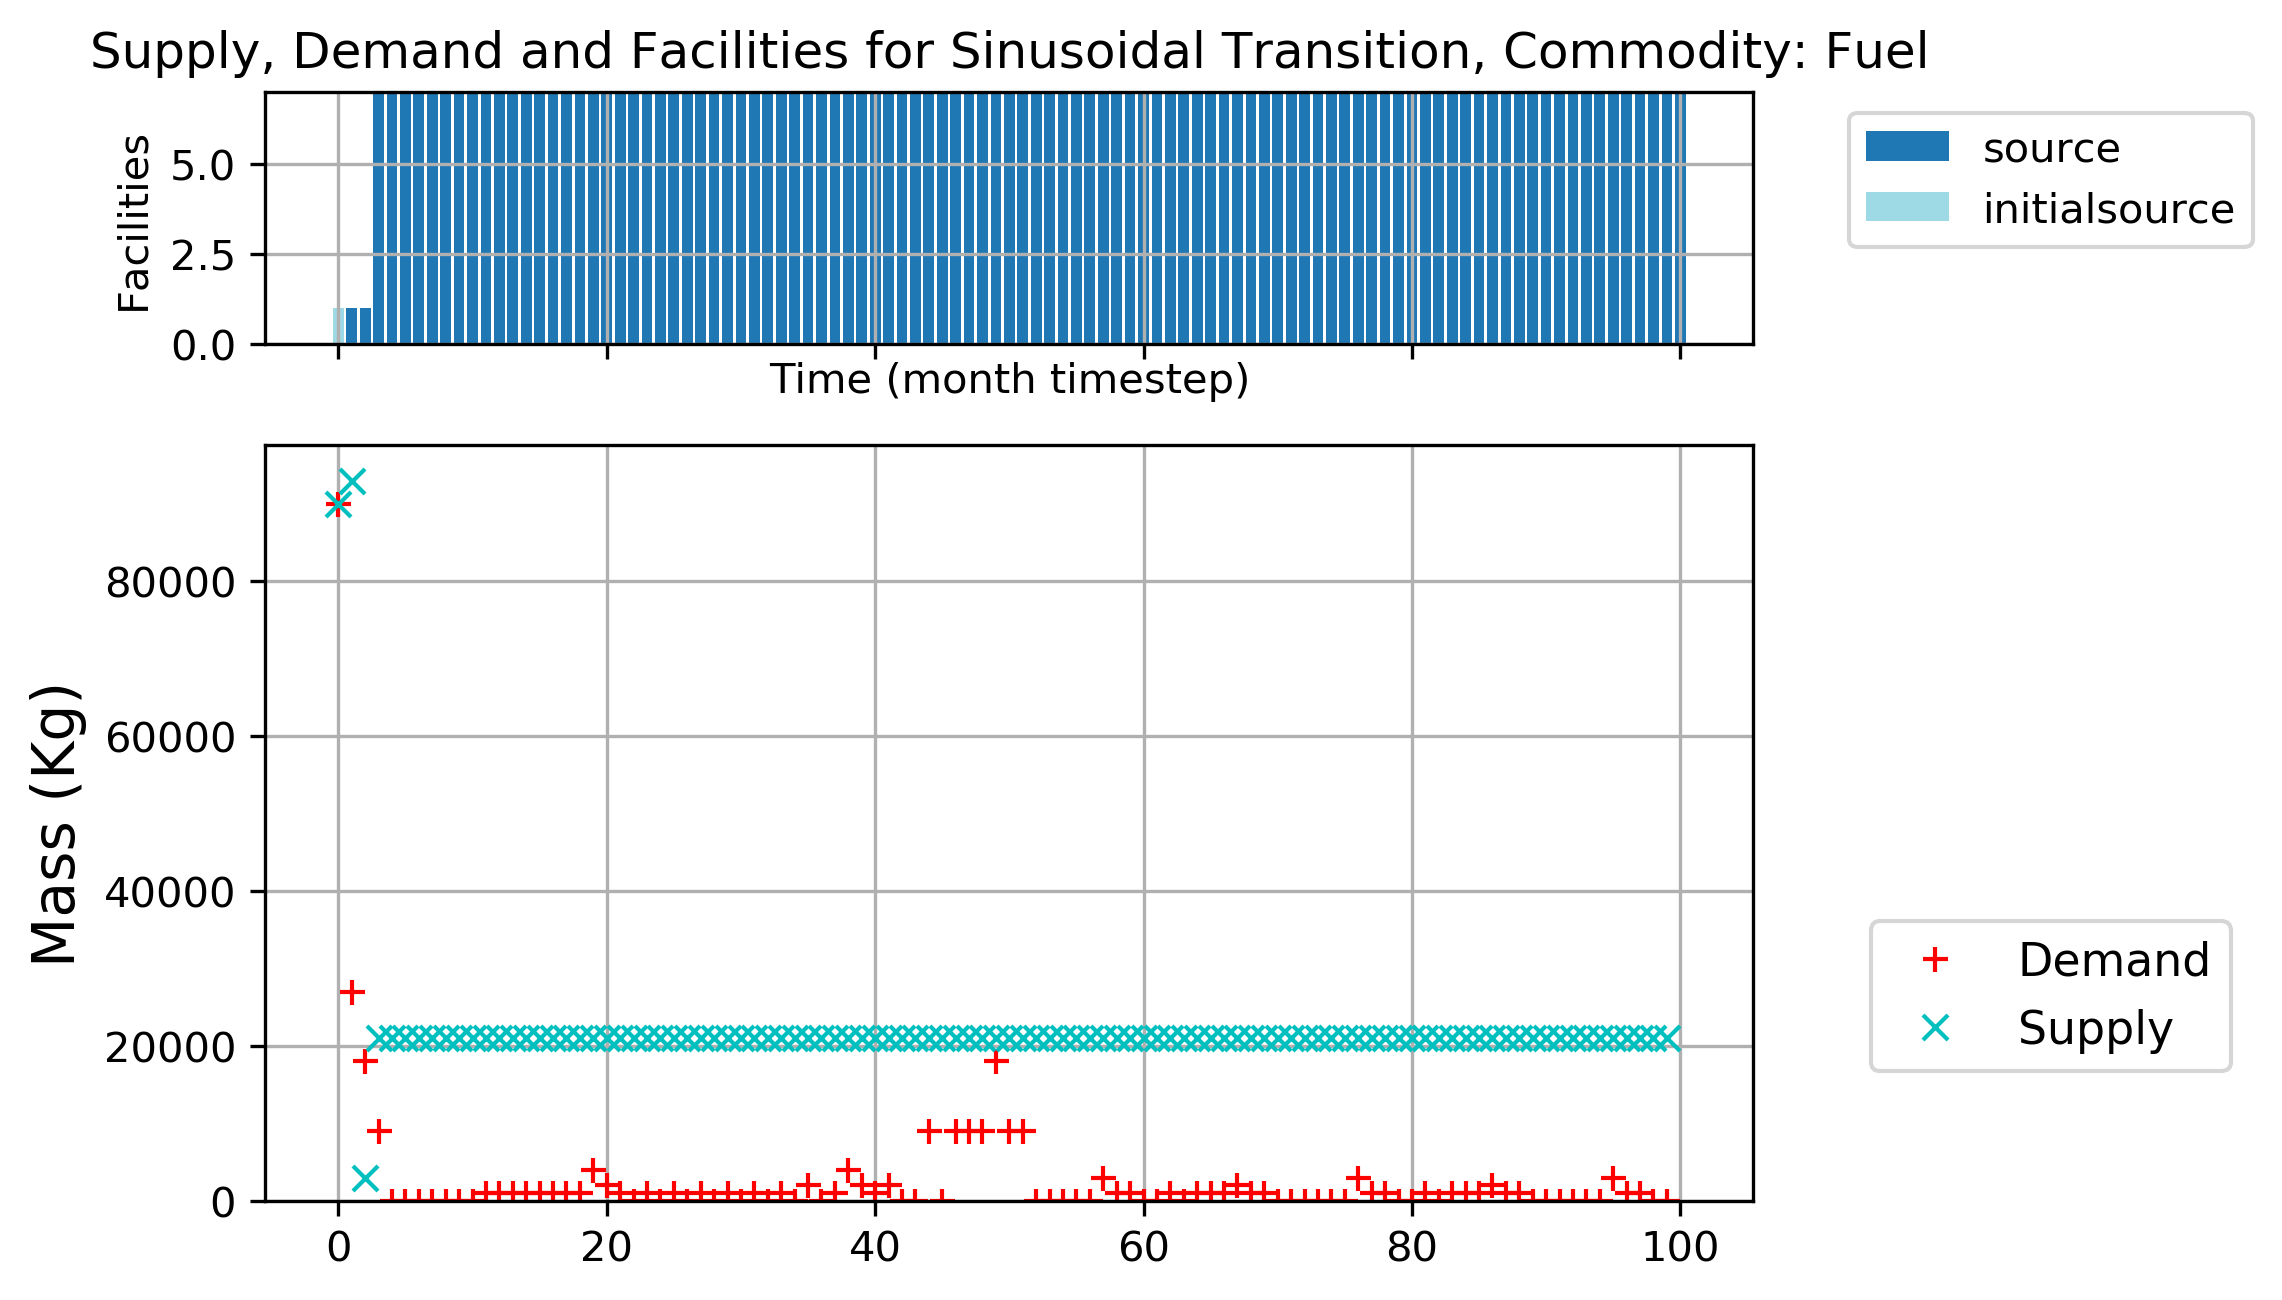
\includegraphics[width=\linewidth]{figures/sinetransition-fuel.png} 
        \caption{Fuel demand and supply plot.}
	    \label{fig:sinetransition-fuel}
    \end{subfigure}
    \hfill
    \begin{subfigure}[t]{0.45\textwidth}
        \centering
        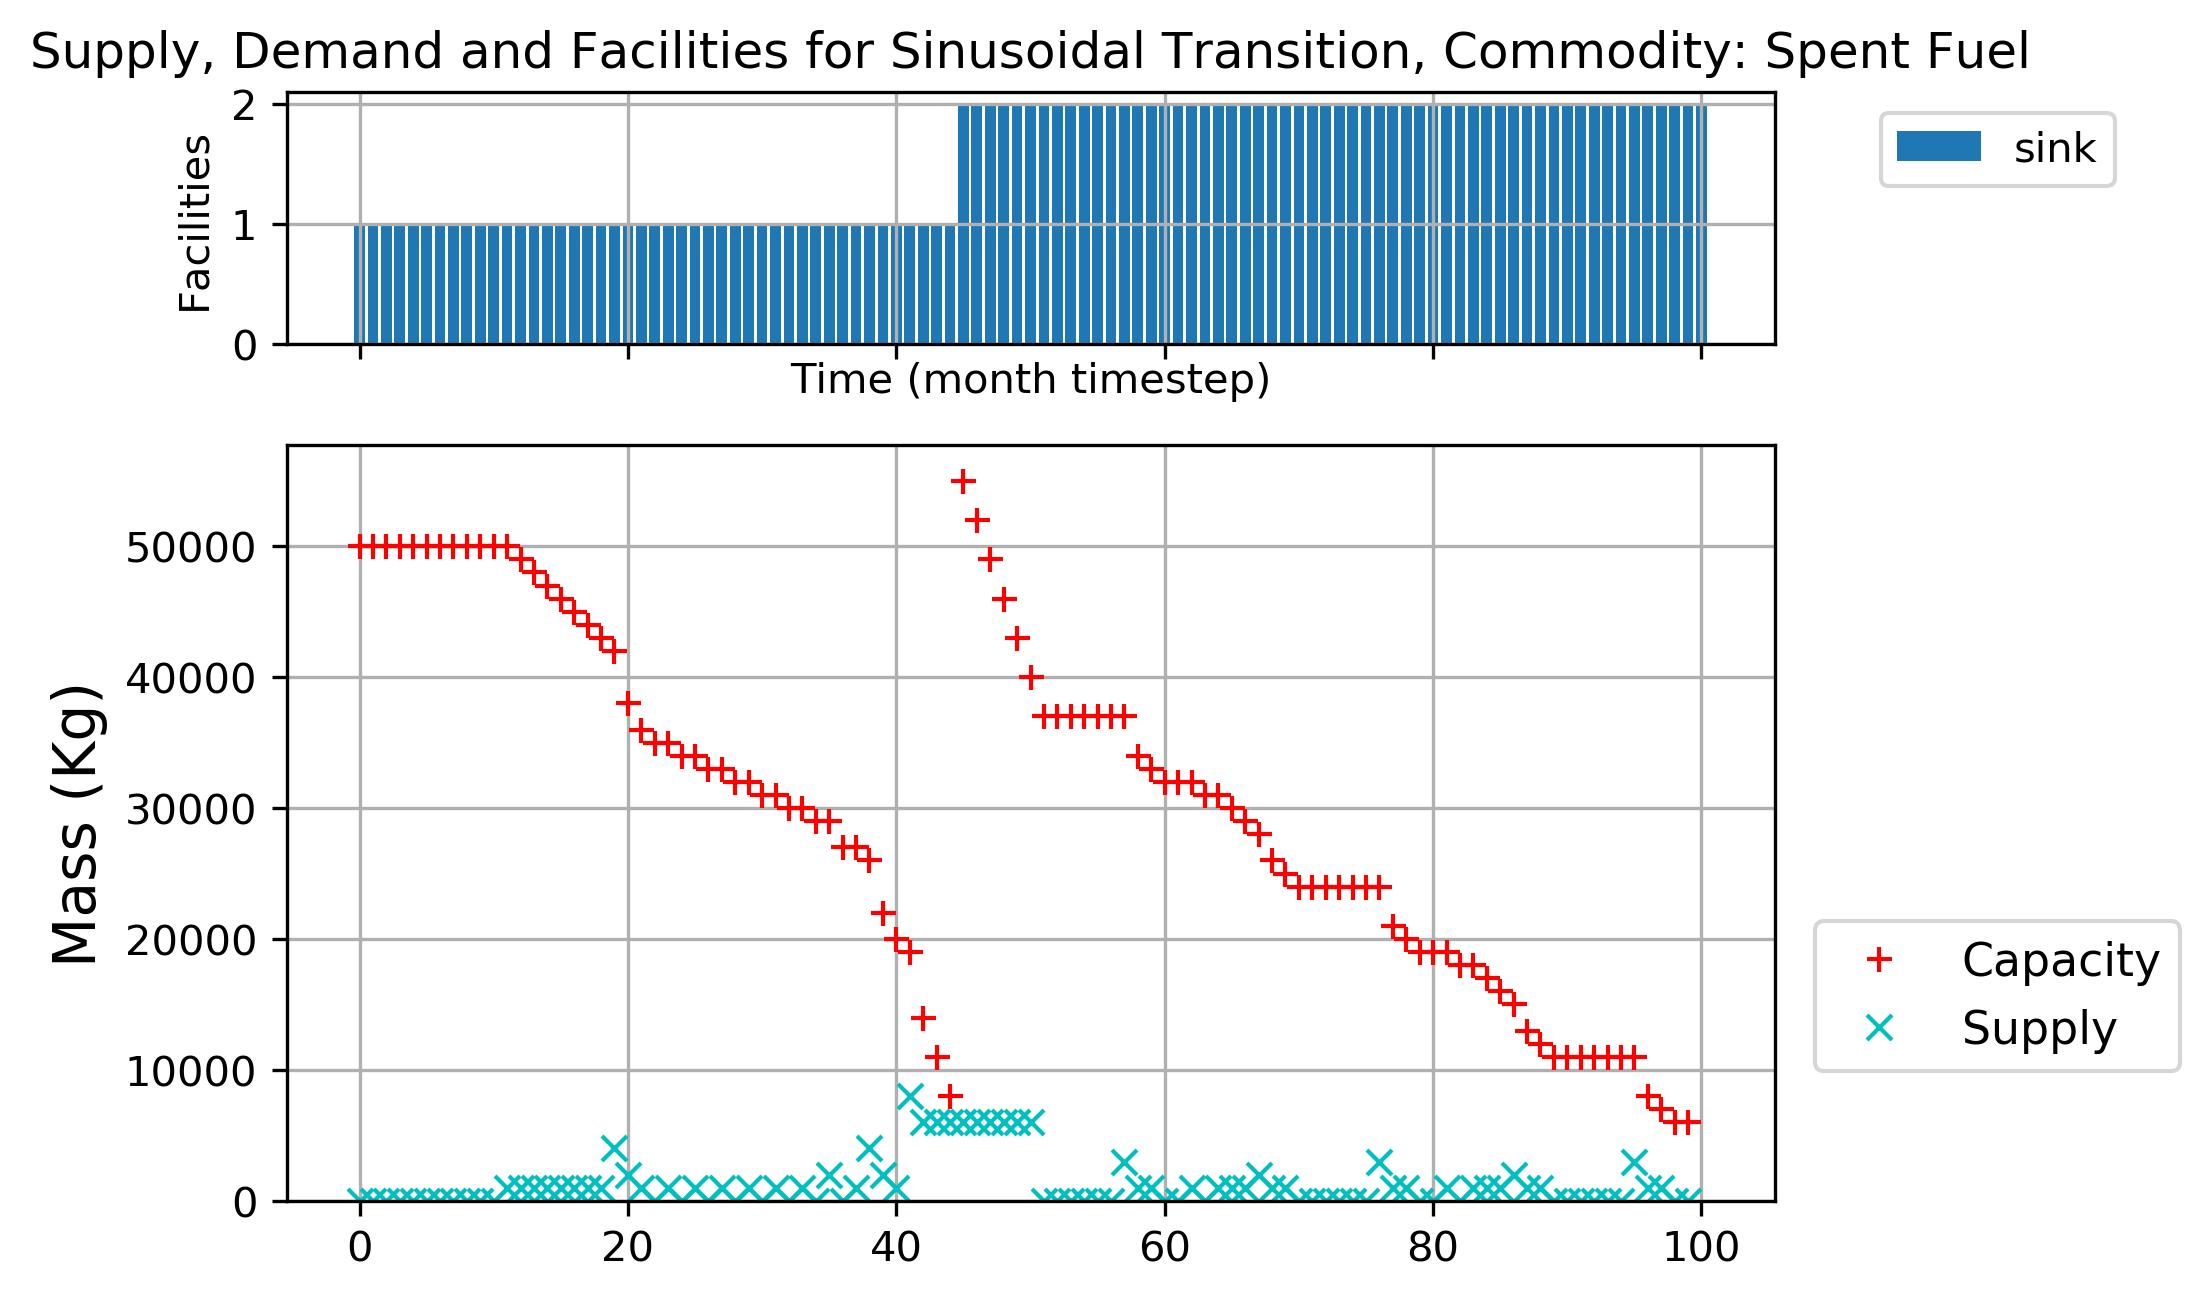
\includegraphics[width=\linewidth]{figures/sinetransition-spentfuel.png} 
        \caption{Spent Fuel demand and supply plot.}
        \label{fig:sinetransition-spentfuel}
    \end{subfigure}
    \caption{Transition Scenario: Sinusoidal Power Demand.}
\end{figure*}

\pagebreak
\section{Transition Scenarios}

The objective of this section was to carry out various simulations to validate 
\texttt{D3ploy}'s current capabilities for simulating complex cycles.
The Idaho National Laboratory Nuclear Fuel Cycle Evaluation and Screening Report \cite{wigeland_nuclear_2014} established several fuel cycle scenarios.
As part of the project NEUP-FY16-10512, the simulations focused on the cases EG01, EG23, EG24. The scenarios started at EG01 -- representing the current U.S. fuel cycle -- and transitioned to advanced fuel cycles.
The simulations utilized \texttt{d3ploy}'s NO, DO, and SO algorithms.

All the analyzed scenarios started at EG01. In EG01 all reactors were LWRs running a  once-through cycle burning enriched-U.
In EG23 fast reactors (FRs) produced all the power, relying on the continuous recycle of U/Pu supplemented by the addition of new natural-U to the cycle.
EG24 was similar to EG23, but its cycle utilized continuous recycling of U/TRU with the addition of new natural-U.

The present work focused on two transition scenarios: EG01-EG23 and EG01-EG24,  as shown in Figure \ref{fig:flow}. The simulations started with a fleet of LWRs. After 80 years, the simulation progressively decommissioned the LWRs while transitioning to FRs. By the end of the cycle, all power was produced by FRs. Initial fueling of the FRs relied on  reprocessed Pu from the LWR fleet. Following the transition, the FRs were able to produce their own Pu to sustain the cycle.

\begin{figure*}[]
	\centering
	\begin{subfigure}[t]{\textwidth}
		\centering
		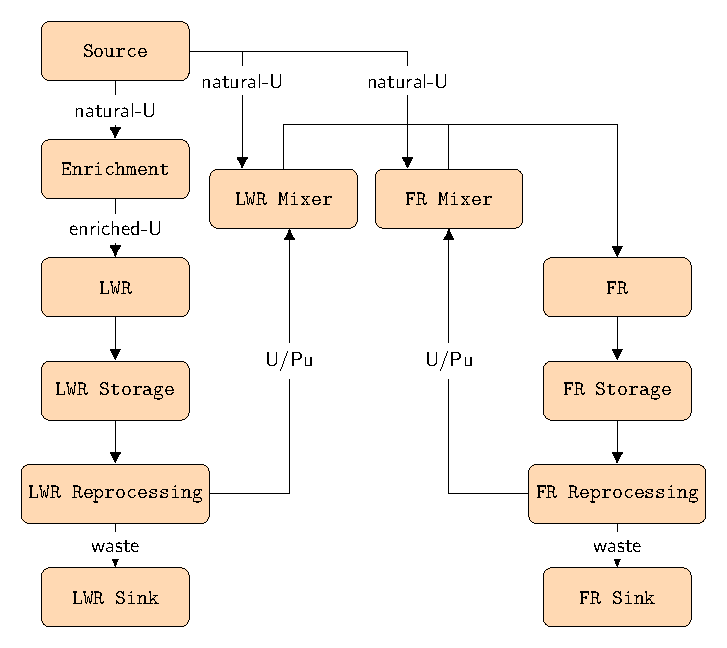
\includegraphics[width=0.7\linewidth]{23flow.pdf} 
		\caption{EG01-EG23.}
		\label{fig:23flow}
	\end{subfigure}
	\vspace{1cm}
	\begin{subfigure}[t]{\textwidth}
		\centering
		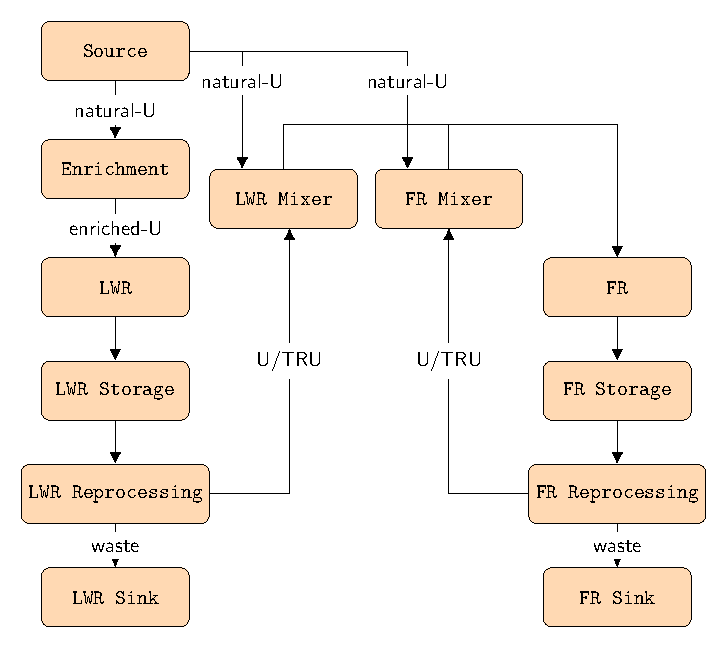
\includegraphics[width=0.7\linewidth]{24flow.pdf} 
		\caption{EG01-EG24.}
		\label{fig:24flow}
	\end{subfigure}
	\hfill
	\caption{Diagrams with facilities and mass flow of the scenarios EG01-EG23 and EG01-EG24.}
	\label{fig:flow}
\end{figure*}

The following section presents the results for EG01-EG23 and EG01-EG24. The power demand was set at a constant 60 GW at all times. The transition scenarios used the capability of deploying facilities based on the difference between predicted demand and predicted supply, using a power supply buffer of 2000 MW. 

This section also includes a sensitivity analysis of the buffer size. A separate sensitivity analysis shows the dependency of the undersupply on the number of previous time steps used to calculate the predicted demand and supply.

\subsection{EG01-EG23}

Figure \ref{fig:23power} shows the power demand and supply obtained using different prediction methods. Following it, Table \ref{tab:23-power} displays a comparison of the different algorithms. Table \ref{tab:23-power} displays the Cumulative Undersupply and the Cumulative Oversupply magnitudes. These values represent the summation of the difference between the power supplied and the power demanded for all the time steps in the simulation. This magnitude could best be thought of as energy. For undersupply conditions, the magnitude represents lack of energy provided during the time steps where the supply did not meet the demand. Likewise, the oversupply would be the magnitude of excess energy produced.

\begin{table*}[!h]
	\centering
	\caption {Undersupply and oversupply of Power for the different algorithms used to calculate EG01-EG23.}
	\label{tab:23-power}
	\begin{tabular}{|l|c|c|c|}
		\hline
		& \multicolumn{3}{c|}{Power} \\ \hline
		Algorithm & \shortstack{No. of time steps\\of undersupply}  & 
		\shortstack{Cumulative\\Undersupply[GW]}  & \shortstack{Cumulative\\Oversupply[GW]} \\ \hline
		MA        & 20 	& 20.0  &  920.5   \\ \hline
		ARMA      & 18 	&  7.7  &  1036.5  \\ \hline
		ARCH      &  0 	&   0  	&  1320.1  \\ \hline
		POLY      &  1 	&  0.3 	&  1783.5  \\ \hline
		EXP\_SMOOTHING 	& 20 	& 11.0 & 1473.5 \\ \hline
		HOLT-WINTERS  	& 20 	& 11.0 & 1473.5 \\ \hline
		FFT       & 2 	& 60.3 	& 1751.9 	\\ \hline
		SW\_SEASONAL    & 20 	& 18.6 	& 1119.9 	\\ \hline
	\end{tabular}
\end{table*}

\begin{table*}[!h]
	\centering
	\caption {No. of time steps with undersupply and under capacity of various commodities for the different algorithms used to calculate EG01-EG23.}
	\label{tab:23-commod}
	\begin{tabular}{|l|c|c|c|c|c|}
		\hline
		& \multicolumn{3}{c|}{Undersupply} & \multicolumn{2}{c|}{Undercapcity} \\ \hline
		Algorithm & Sourceout & Enrichmentout & FR fuel & LWR PU & FR PU \\ \hline
		MA        & 0 & 0 & 0 & 1 & 1 \\ \hline
		ARMA      & 0 & 0 & 0 & 1 & 1 \\ \hline
		ARCH      & 0 & 0 & 0 & 1 & 1 \\ \hline
		POLY      & 0 & 0 & 0 & 1 & 1 \\ \hline
		EXP\_SMOOTHING & 0 & 0 & 0 & 1 & 1 \\ \hline
		HOLT\_WINTERS  & 0 & 0 & 0 & 1 & 1 \\ \hline
		FFT       & 0 & 1 & 0 & 1 & 1 \\ \hline
		SW\_SEASONAL  & 0 & 0 & 0 & 1 & 1 \\ \hline
	\end{tabular}
\end{table*}

Table \ref{tab:23-commod} presents the no. of time steps with undersupply of natural-U (sourceout), enriched-U (enrichmentout), and FR fuel. The table also displays the no. of time steps where the capacity of the LWR Mixer to process LWR Pu and the capacity of the FR Mixer to process FR Pu are not enough (undercapacity). In this table it is possible to note that there is one time step of delay between the supply of Pu and the deployment of the respective mixer facility.

\begin{figure*}[!htbp]
	\centering
	\begin{subfigure}[t]{.95\textwidth}
		\centering
		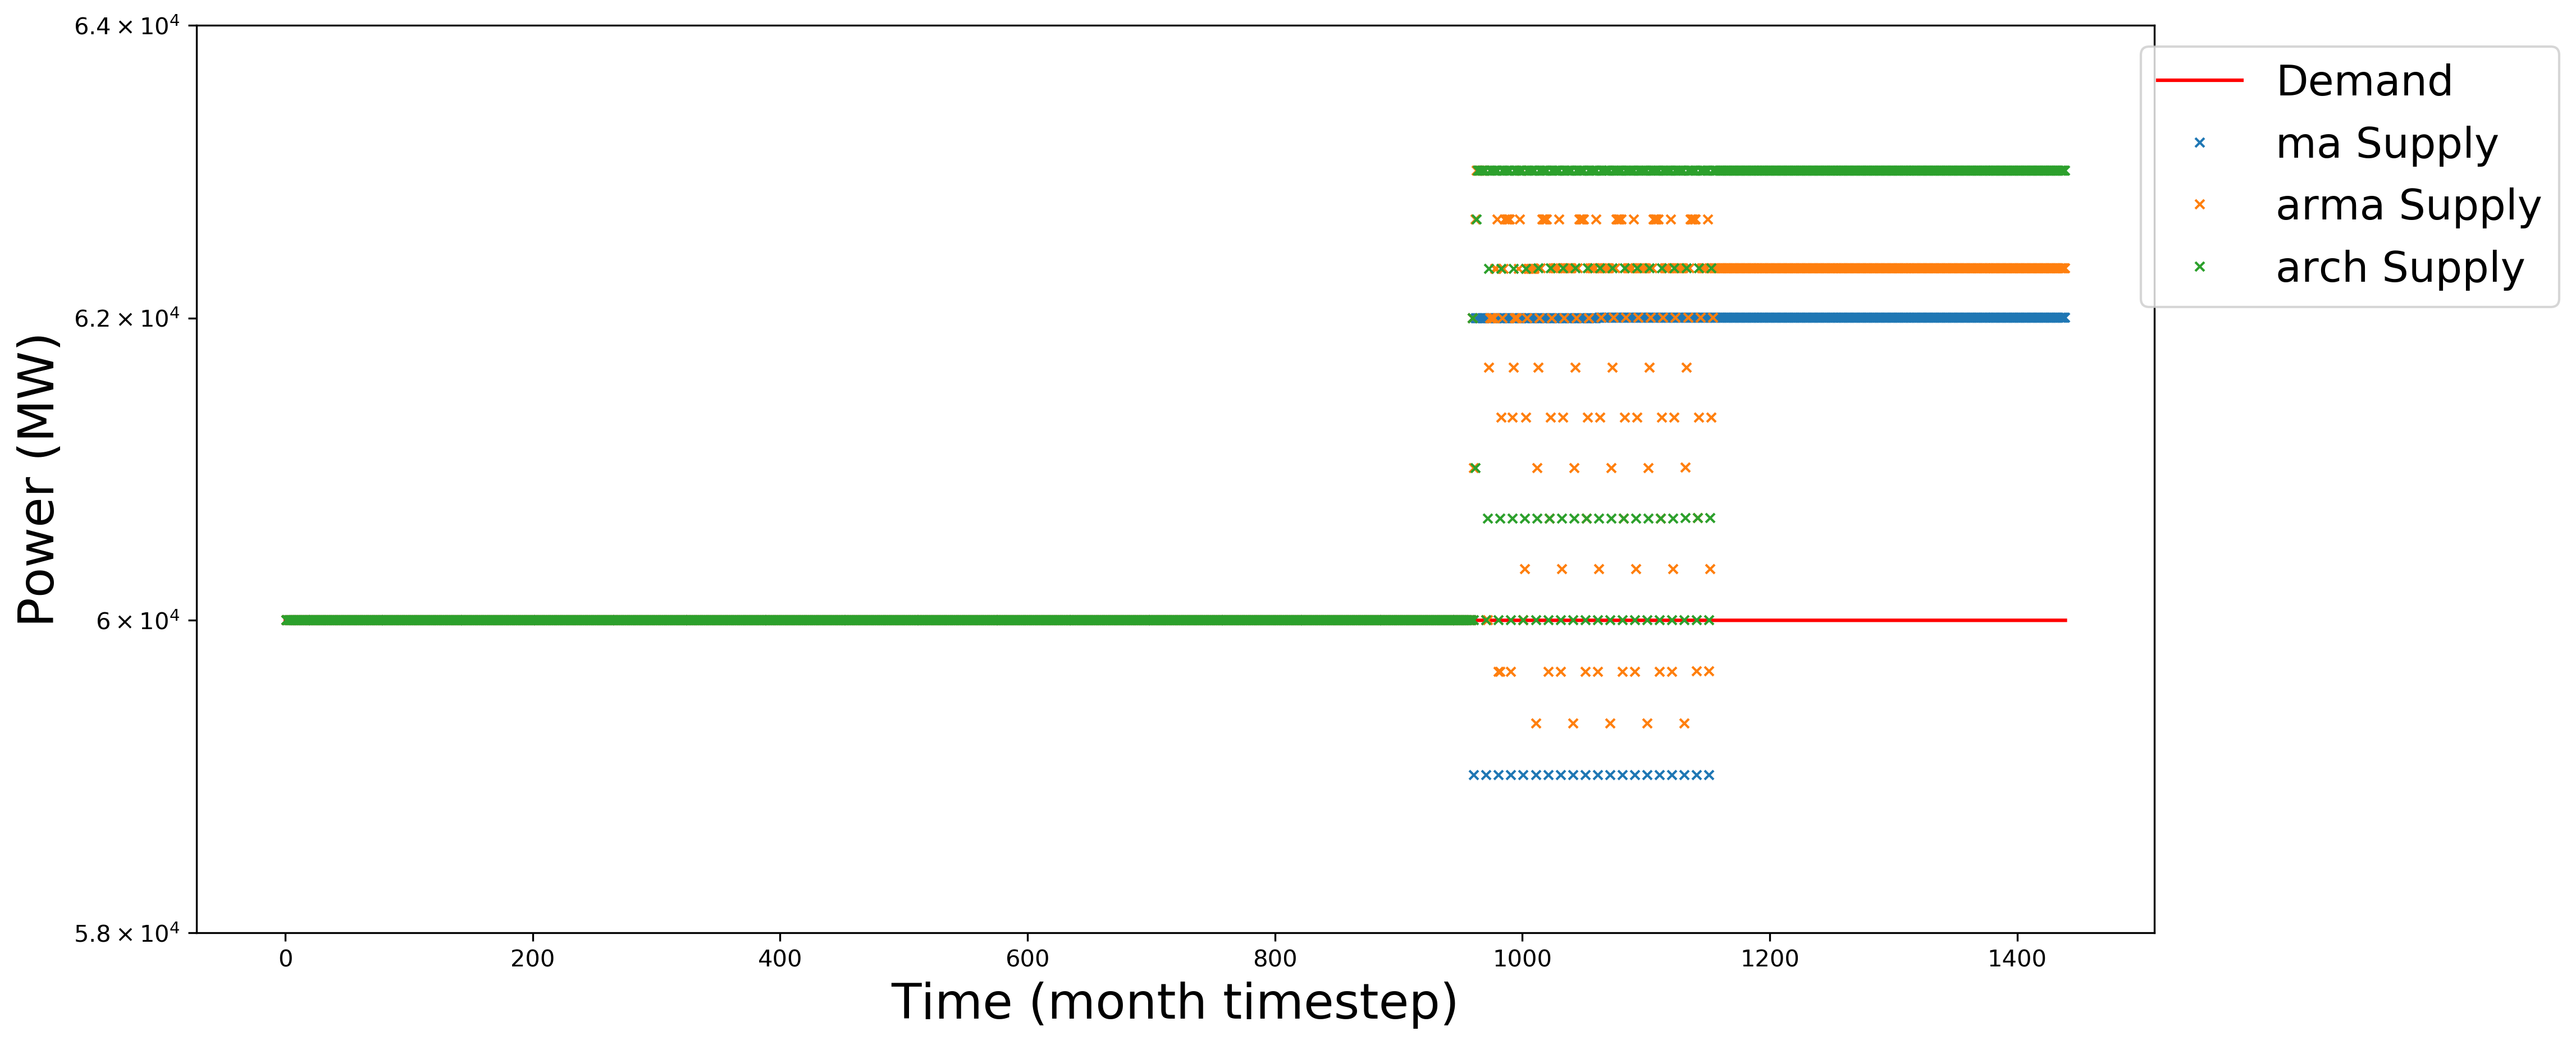
\includegraphics[width=\linewidth]{23-power-bufferB20001.png} 
		\caption{NO algorithms.}
		\label{fig:23powerNO}
	\end{subfigure}
	\vspace{.9cm}
	\begin{subfigure}[t]{.95\textwidth}
		\centering
		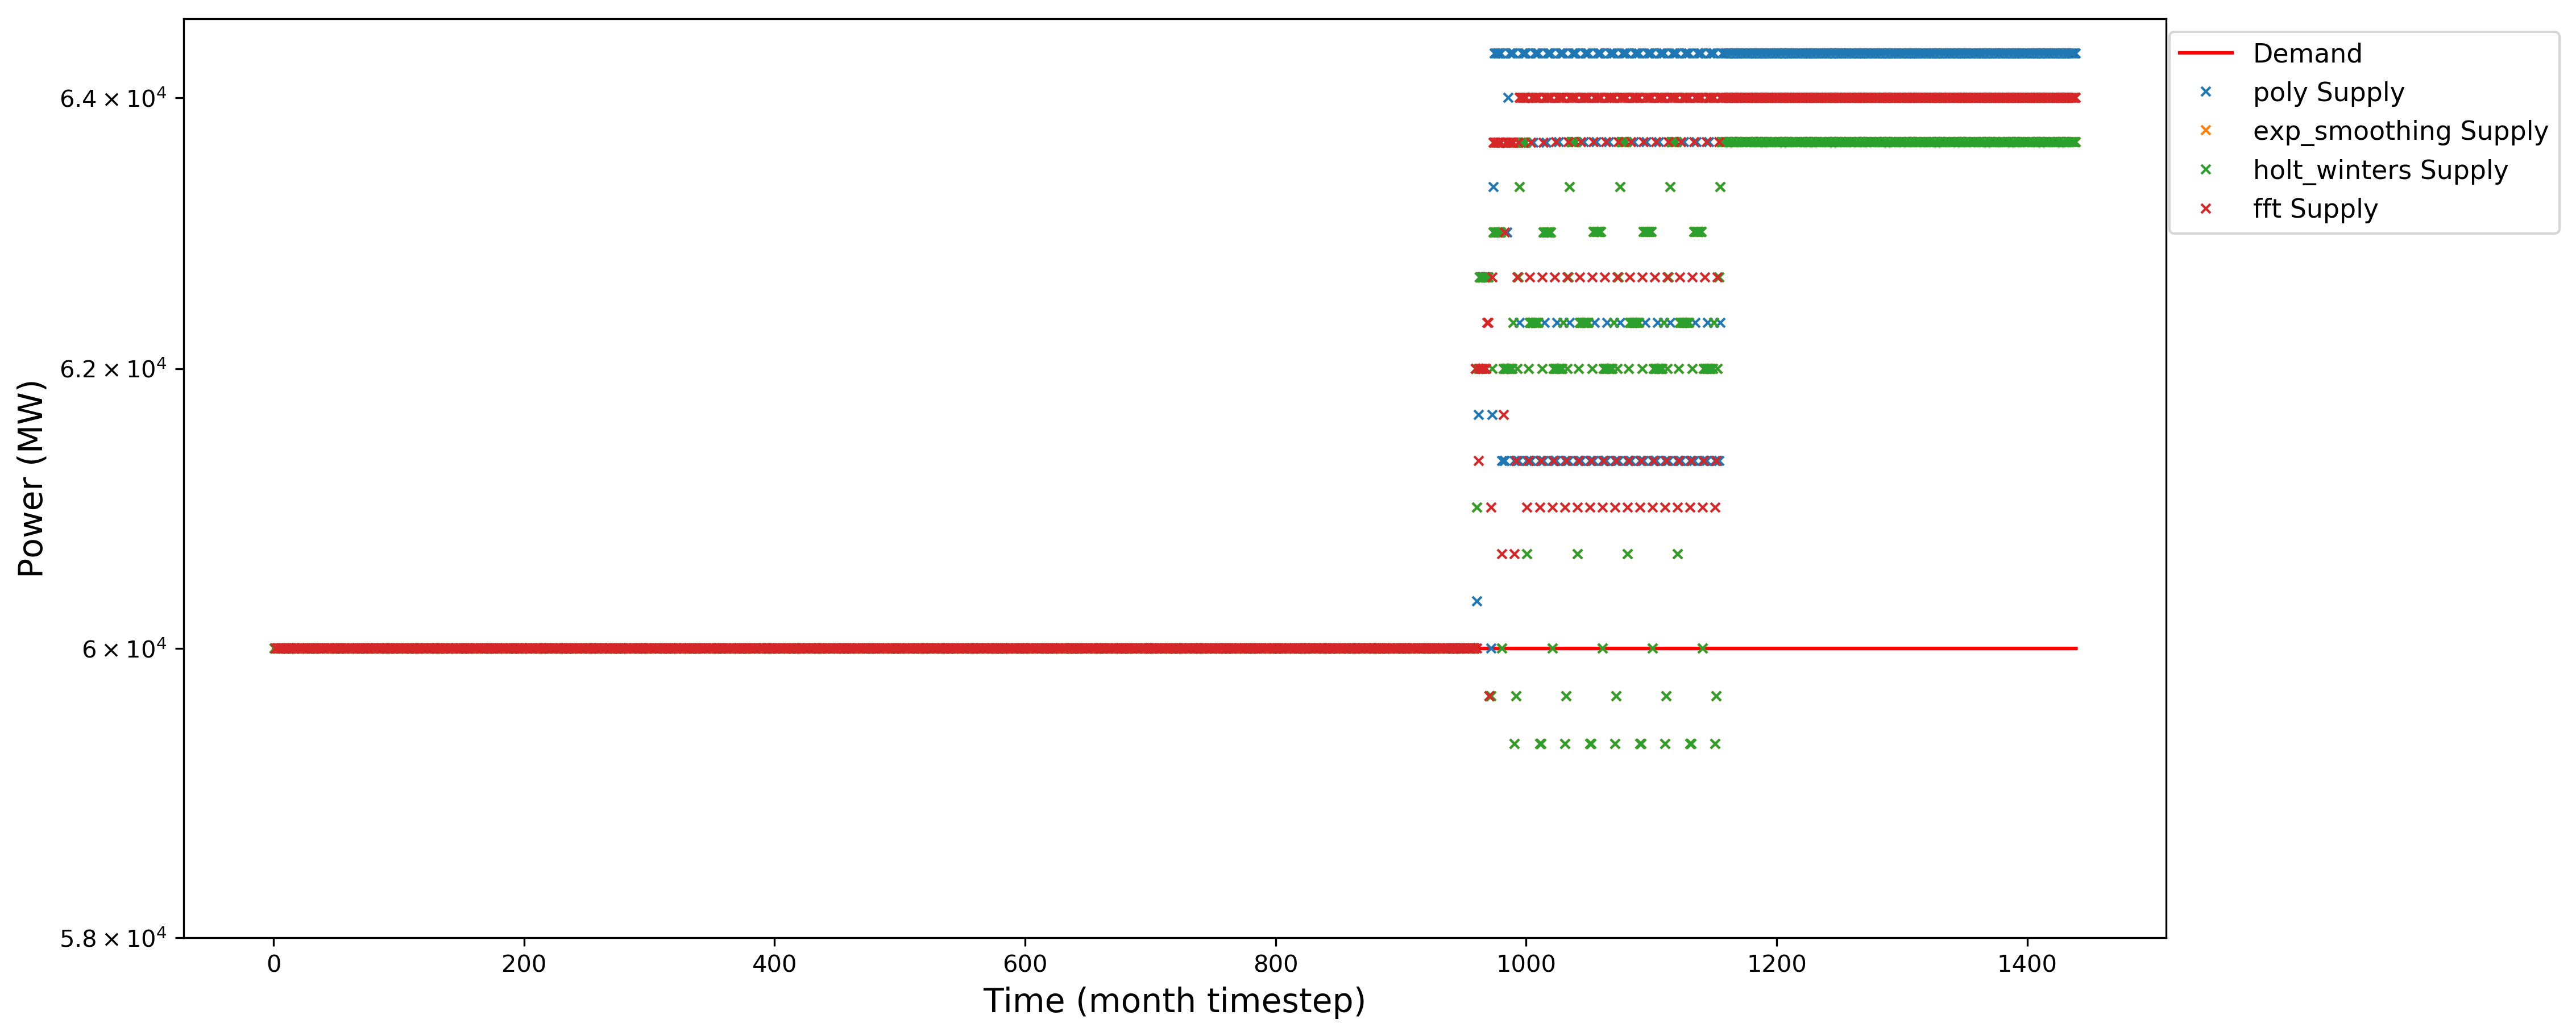
\includegraphics[width=\linewidth]{23-power-bufferB20002.png} 
		\caption{DO algorithms.}
		\label{fig:23powerDO}
	\end{subfigure}
	\vspace{.1cm}
	\begin{subfigure}[t]{.95\textwidth}
		\centering
		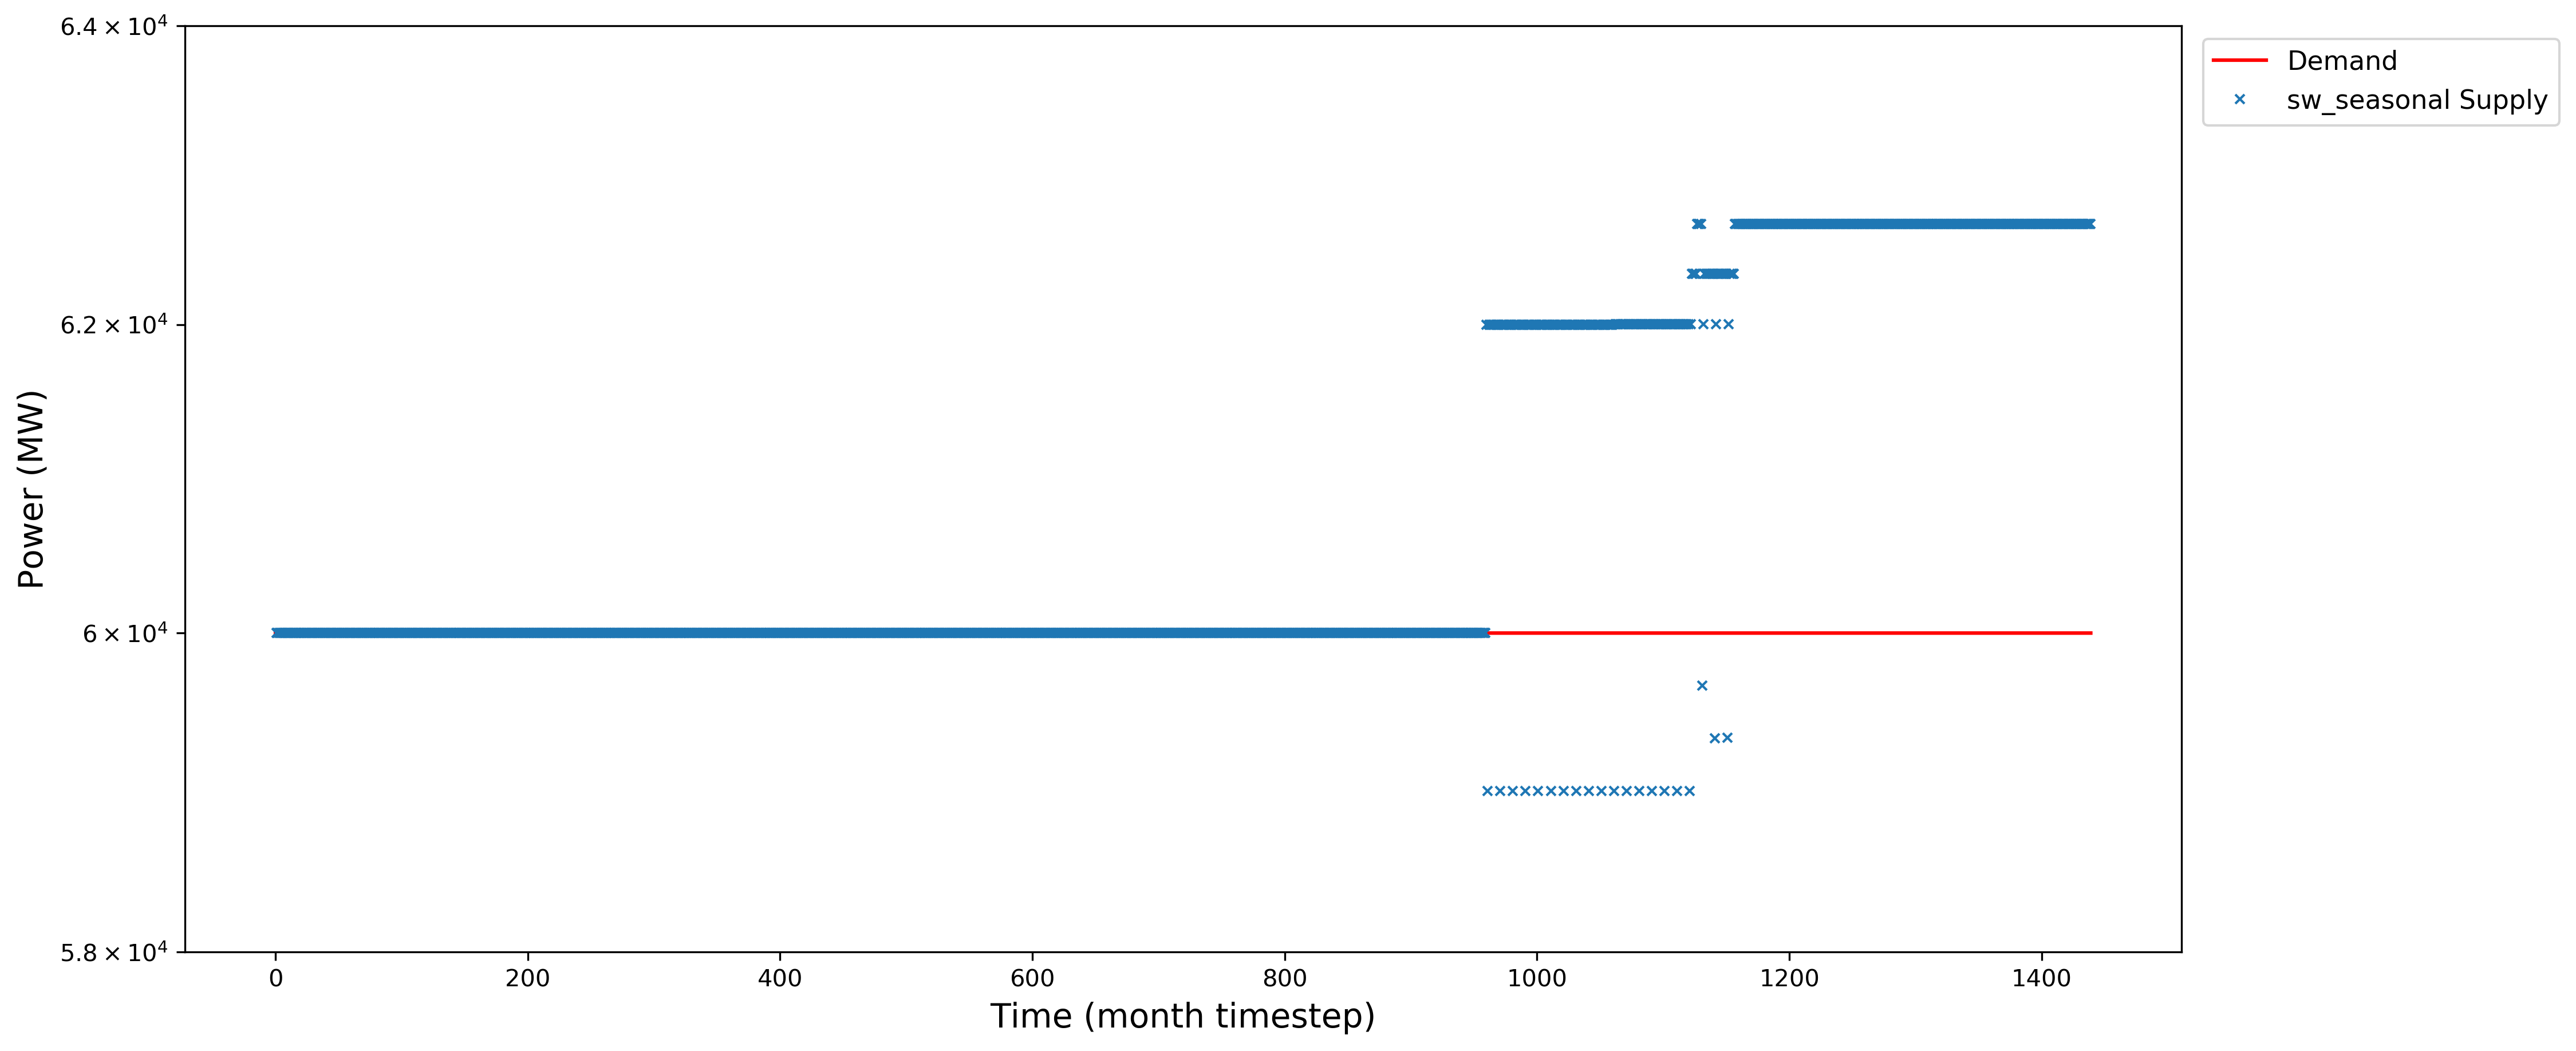
\includegraphics[width=\linewidth]{23-power-bufferB20003.png} 
		\caption{SO algorithms.}
		\label{fig:23powerSO}
	\end{subfigure}
	\hfill
	\caption{Plot of the power demand and supply of EG01-EG23 for a constant power demand of 60GW for different prediction algorithms.}
	\label{fig:23power}
\end{figure*}

One of the methods that performs the better is ARCH. For this scenario and said method, Figure \ref{fig:23-arch-commod} presents some of the different supply and demand time series plots for various commodities.

Figure \ref{fig:23-arch-sourceout} presents the number of Source facilities deployed, and the resultant demand and supply of natural-U. For this case, the capacity of natural-U supply is higher than the demand. It is easy to note that the demand in the beginning of the simulation is higher than in the end. The LWRs use enriched-U produced by the enrichment of natural-U, while the FRs require a smaller quantity of U for their fuel. Figure \ref{fig:23-arch-lwrpu} displays the number of LWR Mixers deployed, and the supply and the capacity of LWR Pu (Pu produced by the LWRs). Logically, the supply of Pu decreases as the LWRs are decommissioned. Figure \ref{fig:23-arch-frpu} shows the FR Mixers, and the supply and capacity of FR Pu. The supply of Pu increases as \deploy deploys new FRs.

\begin{figure*}[!htbp]
	\centering
	\begin{subfigure}[t]{.8\textwidth}
		\centering
		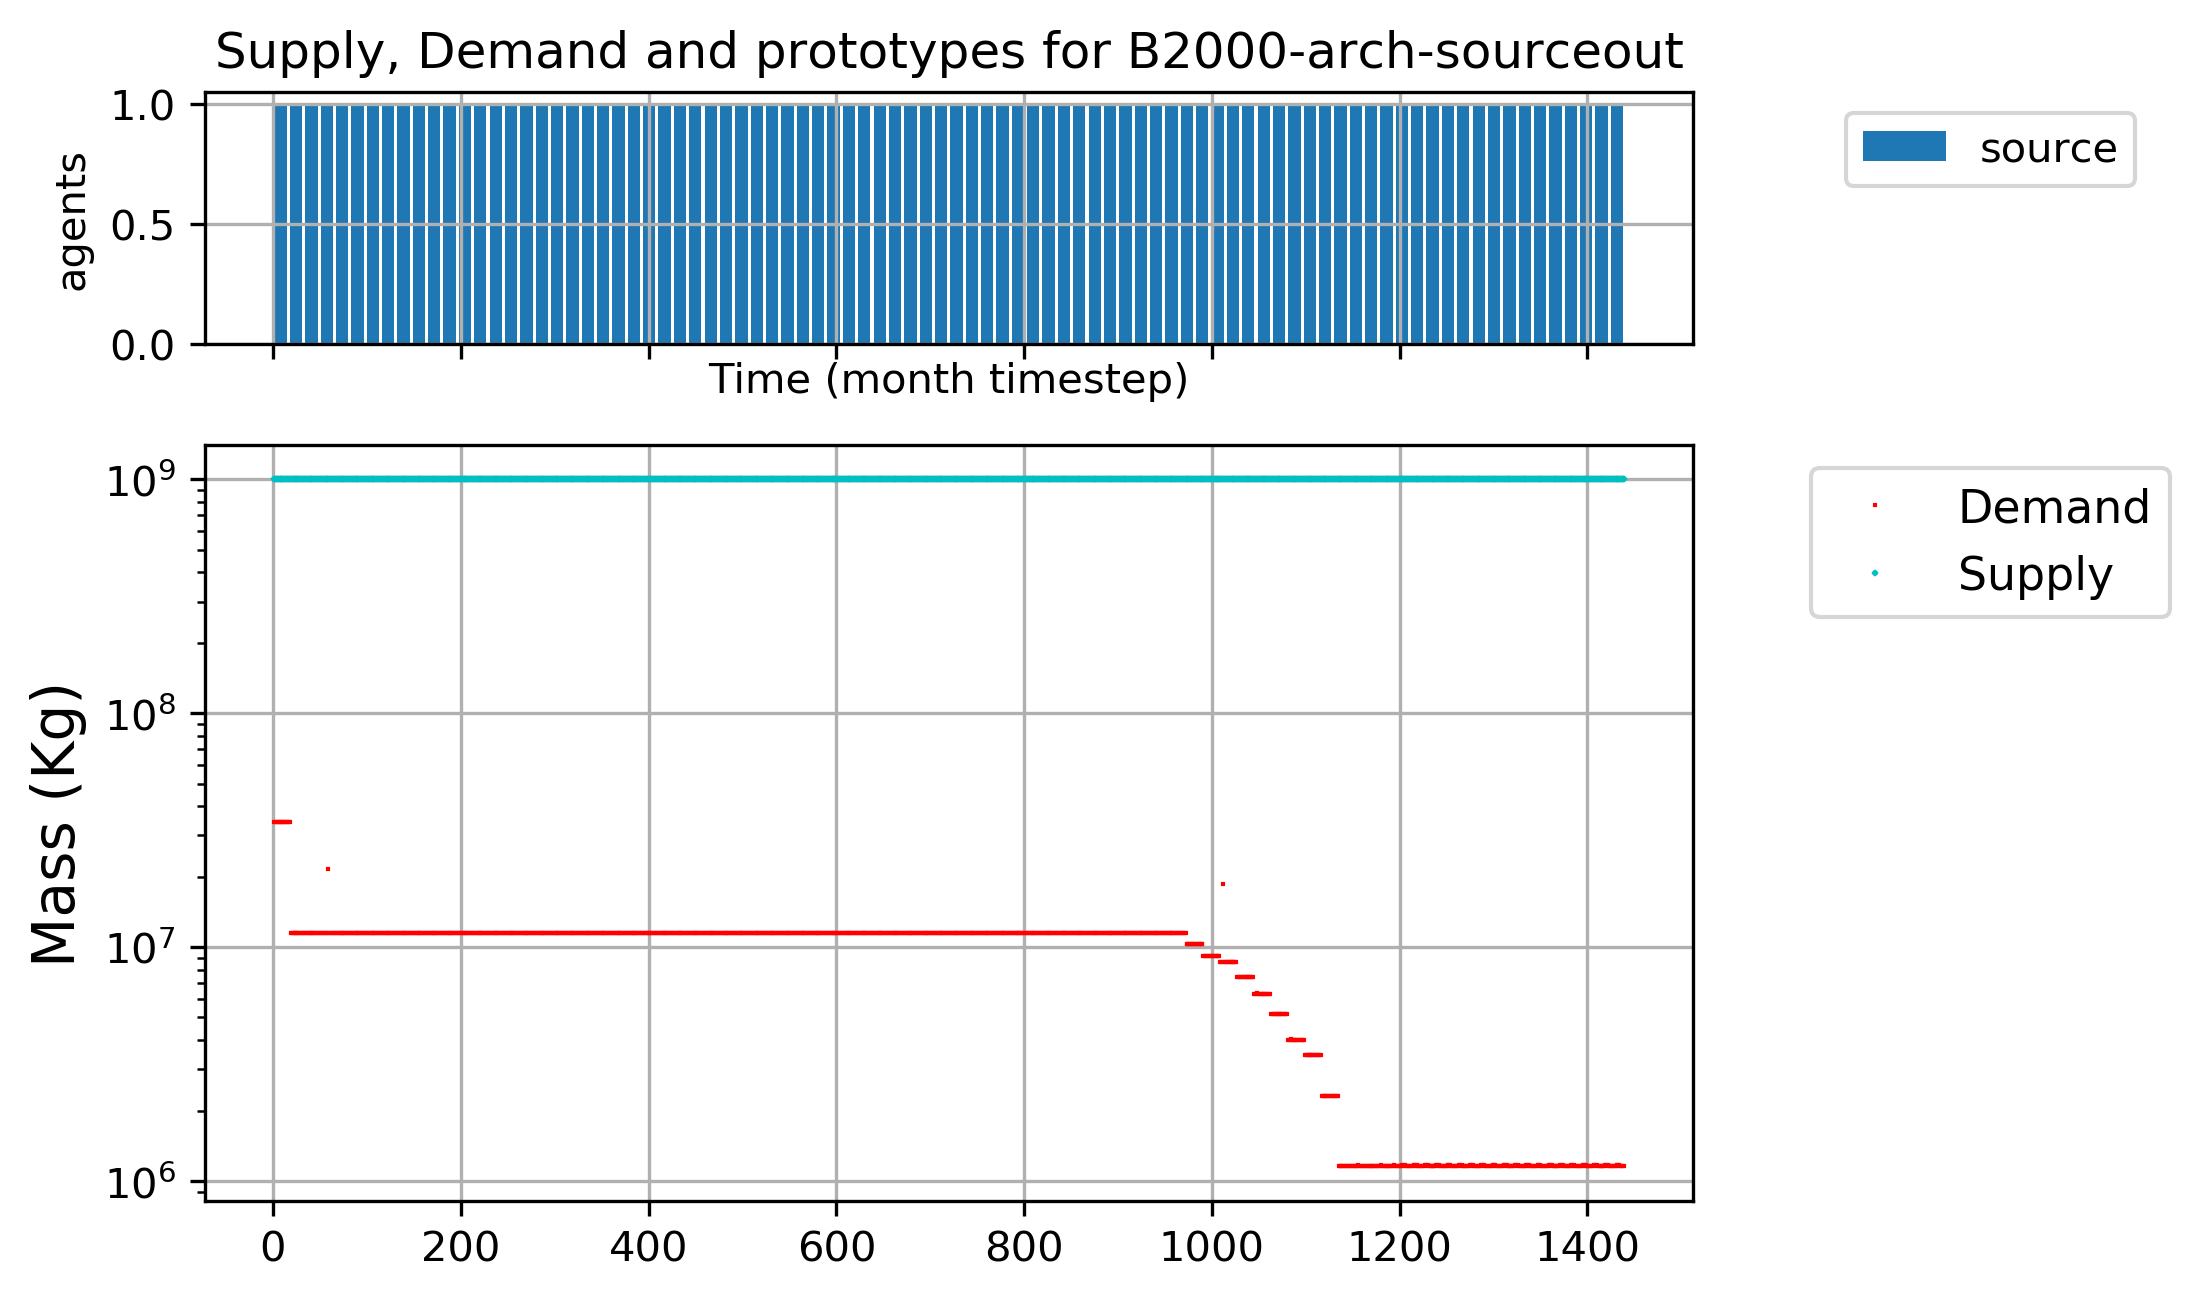
\includegraphics[width=\linewidth]{B2000-arch-sourceout.png} 
		\caption{Production of natural-U by the source.}
		\label{fig:23-arch-sourceout}
	\end{subfigure}
	\vspace{.9cm}
	\begin{subfigure}[t]{.45\textwidth}
		\centering
		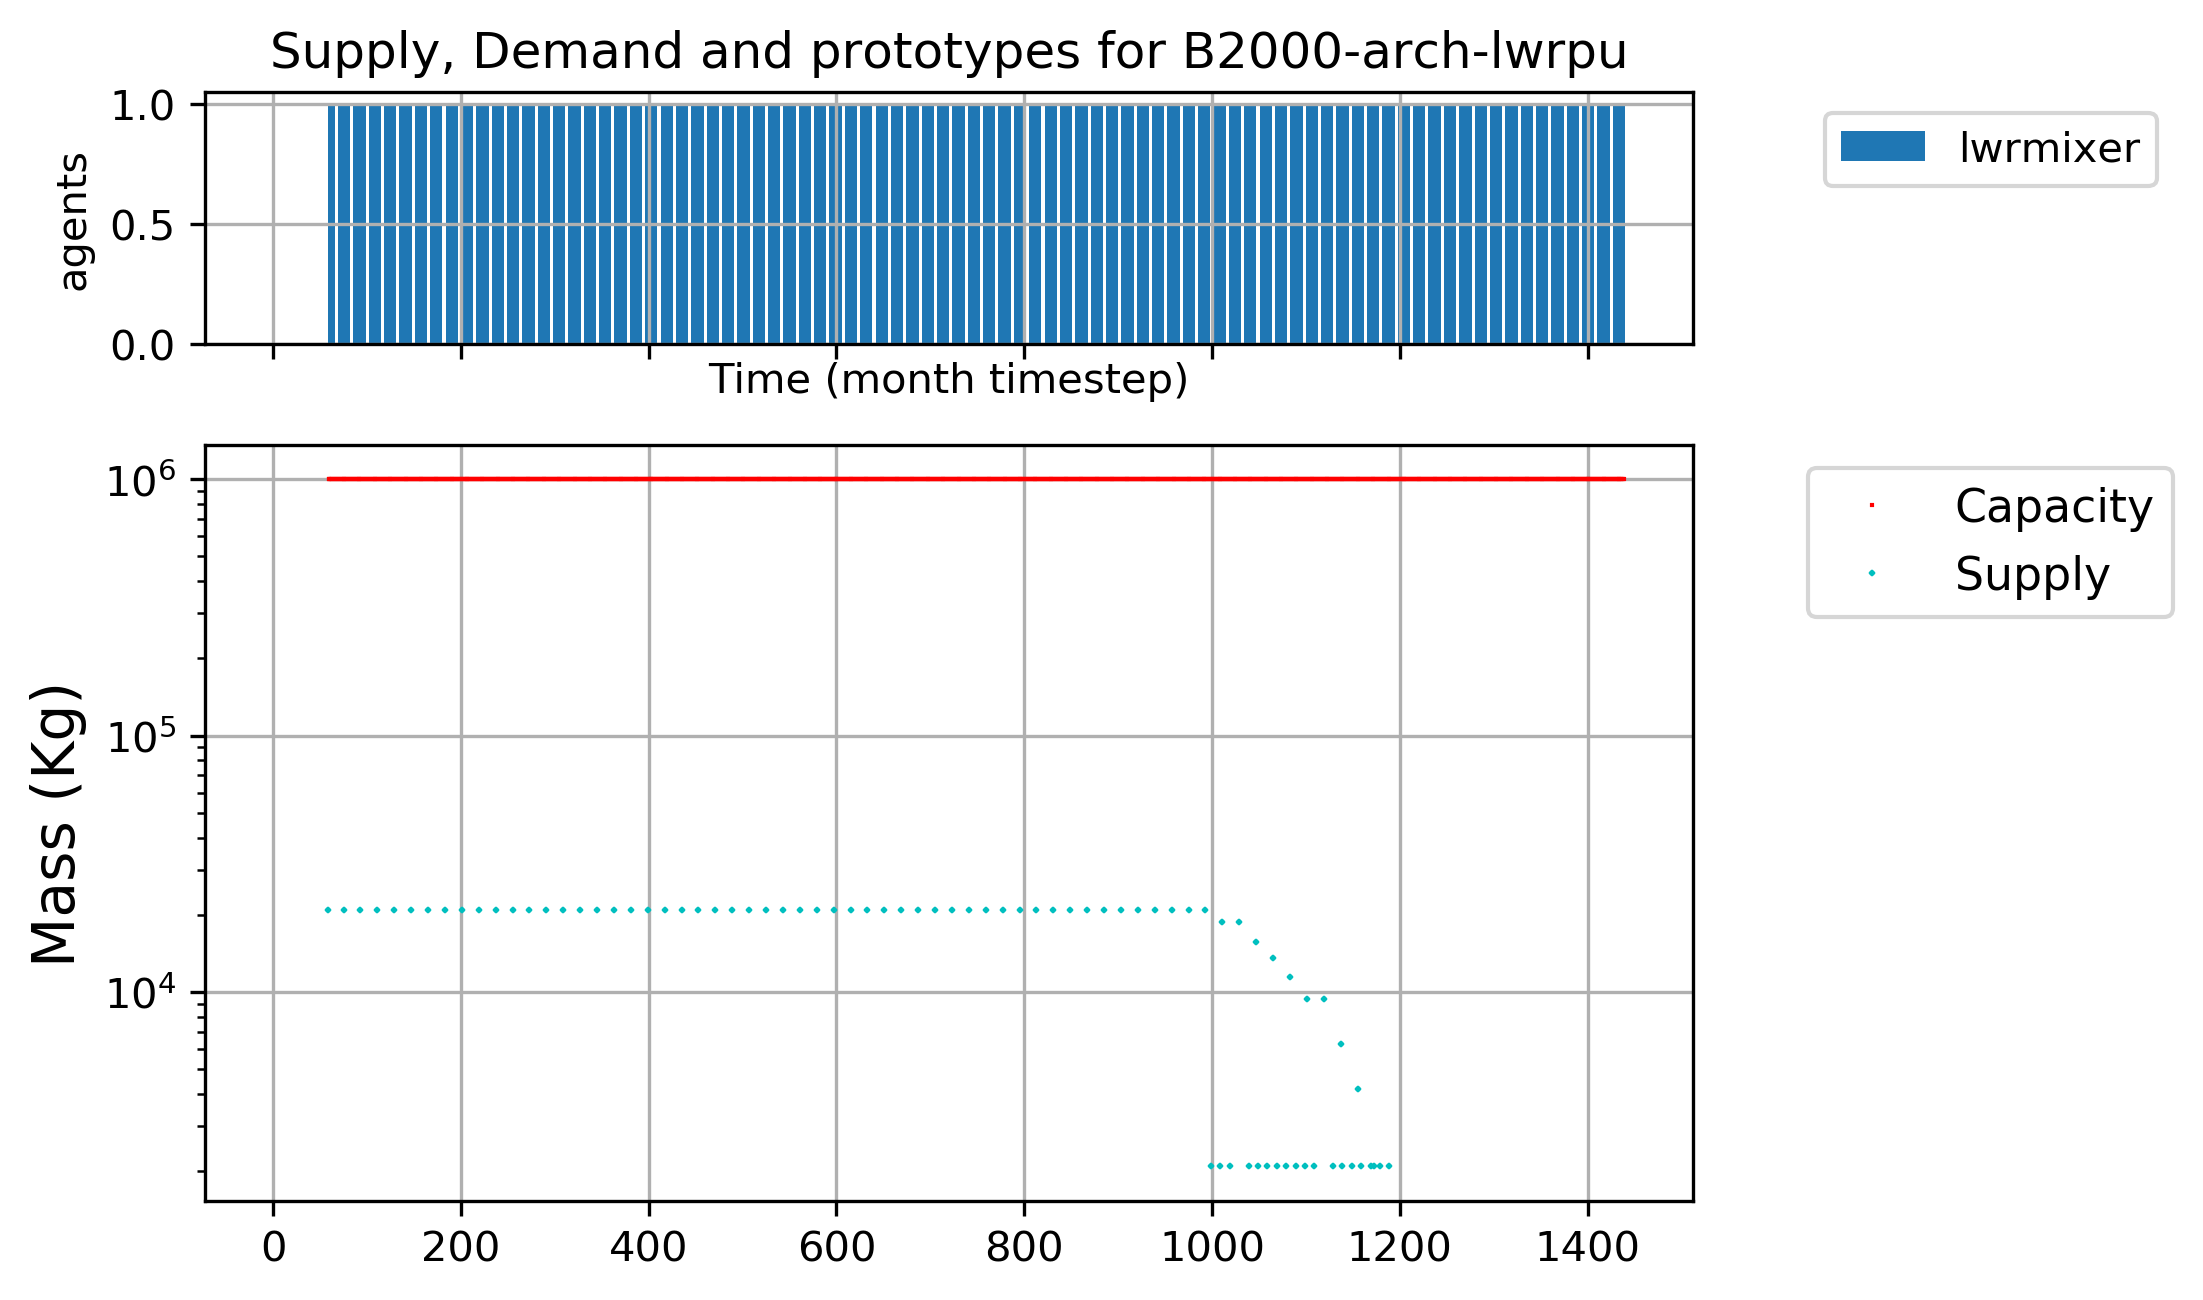
\includegraphics[width=\linewidth]{B2000-arch-lwrpu.png} 
		\caption{Pu produced by the LWRs and exchanged to the LWR Mixer.}
		\label{fig:23-arch-lwrpu}
	\end{subfigure}
	\begin{subfigure}[t]{.45\textwidth}
	\centering
	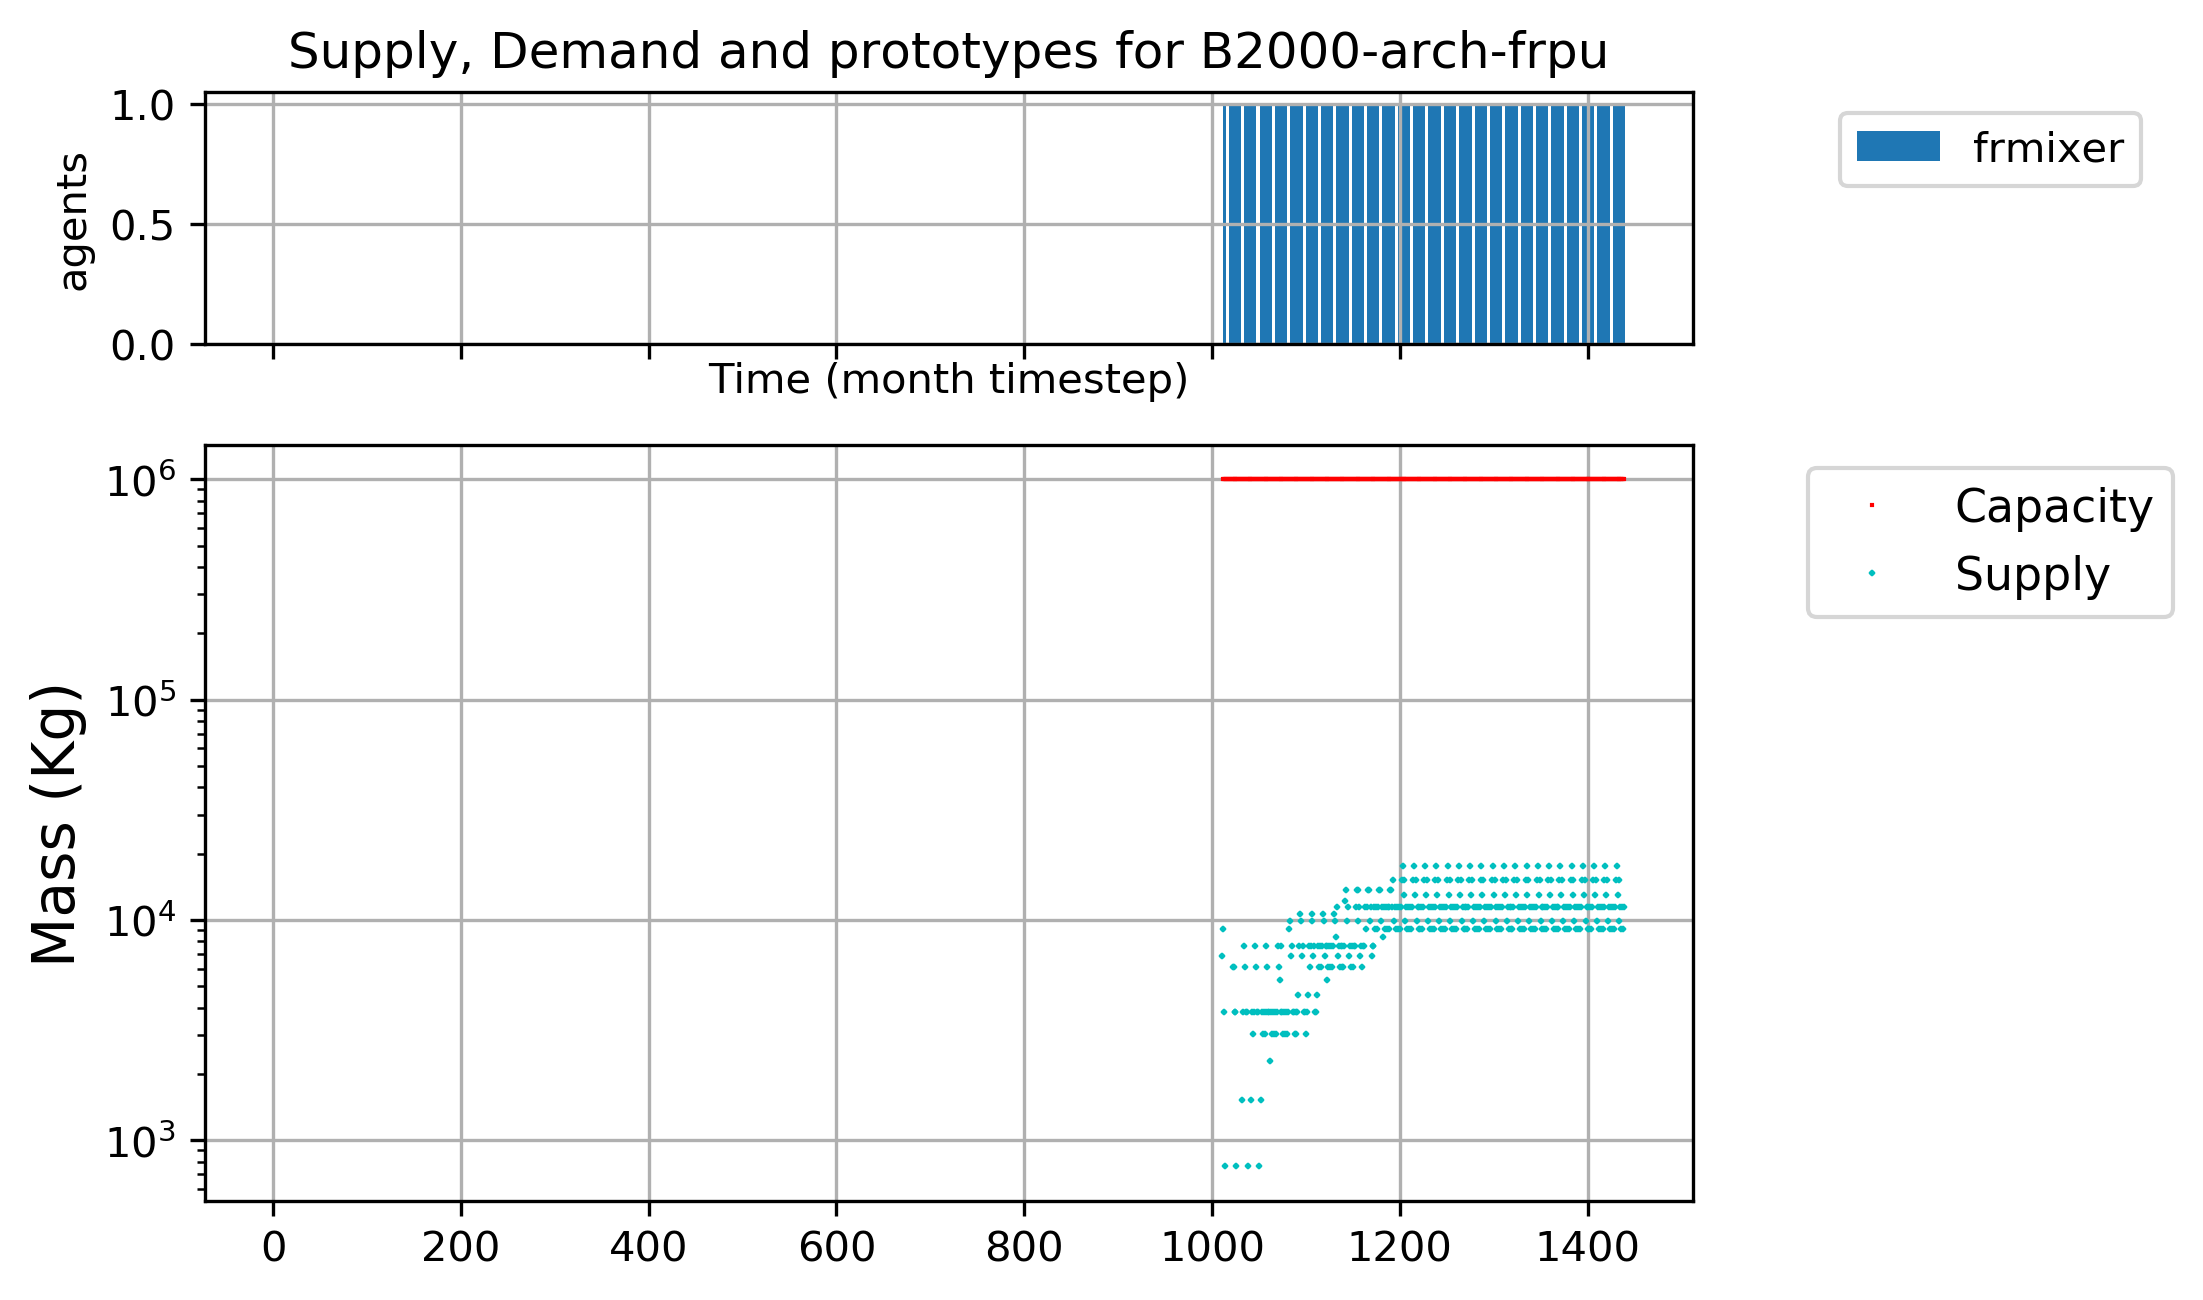
\includegraphics[width=\linewidth]{B2000-arch-frpu.png} 
	\caption{Pu produced by the FRs and exchanged to the FR Mixer.}
	\label{fig:23-arch-frpu}
\end{subfigure}
	\hfill
	\caption{Plot for different commodities EG01-EG23.}
	\label{fig:23-arch-commod}
\end{figure*}

\subsection{EG01-EG24}

Figure \ref{fig:24power} shows the power demand and supply obtained using different prediction methods. Following it, Tables \ref{tab:24-power} and \ref{tab:24-commod} display a comparison of the different algorithms.

\begin{table*}[!h]
	\centering
	\caption {Undersupply and oversupply of Power for the different algorithms used to calculate EG01-EG24.}
	\label{tab:24-power}
	\begin{tabular}{|l|c|c|c|}
		\hline
		& \multicolumn{3}{c|}{Power} \\ \hline
		Algorithm & \shortstack{No. of time steps\\of undersupply}  & 
		\shortstack{Cumulative\\Undersupply[GW]}  & \shortstack{Cumulative\\Oversupply[GW]} \\ \hline
		MA        & 20 	& 20.0  &  920.5   \\ \hline
		ARMA      & 18 	&  7.7  &  1036.5  \\ \hline
		ARCH      &  0 	&   0  	&  1320.1  \\ \hline
		POLY      &  1 	&  0.3 	&  1783.5  \\ \hline
		EXP\_SMOOTHING 	& 20 	& 11.0 & 1473.5 \\ \hline
		HOLT-WINTERS  	& 20 	& 11.0 & 1473.5 \\ \hline
		FFT       & 2 	& 60.3 	& 1751.9	\\ \hline
		SW\_SEASONAL    & 20 	& 18.6 	& 1119.9 	\\ \hline
	\end{tabular}
\end{table*}

\begin{table*}[!h]
	\centering
	\caption {No. of time steps with undersupply and under capacity of various commodities for the different algorithms used to calculate EG01-EG24.}
	\label{tab:24-commod}
	\begin{tabular}{|l|c|c|c|c|c|}
		\hline
		& \multicolumn{3}{c|}{Undersupply} & \multicolumn{2}{c|}{Undercapcity} \\ \hline
		Algorithm & Sourceout & Enrichmentout & FR fuel & LWR PU & FR PU \\ \hline
		MA        & 0 & 0 & 0 & 1 & 1 \\ \hline
		ARMA      & 0 & 0 & 0 & 1 & 1 \\ \hline
		ARCH      & 0 & 0 & 0 & 1 & 1 \\ \hline
		POLY      & 0 & 0 & 0 & 1 & 1 \\ \hline
		EXP\_SMOOTHING & 0 & 0 & 0 & 1 & 1 \\ \hline
		HOLT\_WINTERS  & 0 & 0 & 0 & 1 & 1 \\ \hline
		FFT       & 0 & 1 & 0 & 1 & 1 \\ \hline
		SW\_SEASONAL  & 0 & 0 & 0 & 1 & 1 \\ \hline
	\end{tabular}
\end{table*}

\begin{figure*}[!htbp]
	\centering
	\begin{subfigure}[t]{\textwidth}
		\centering
		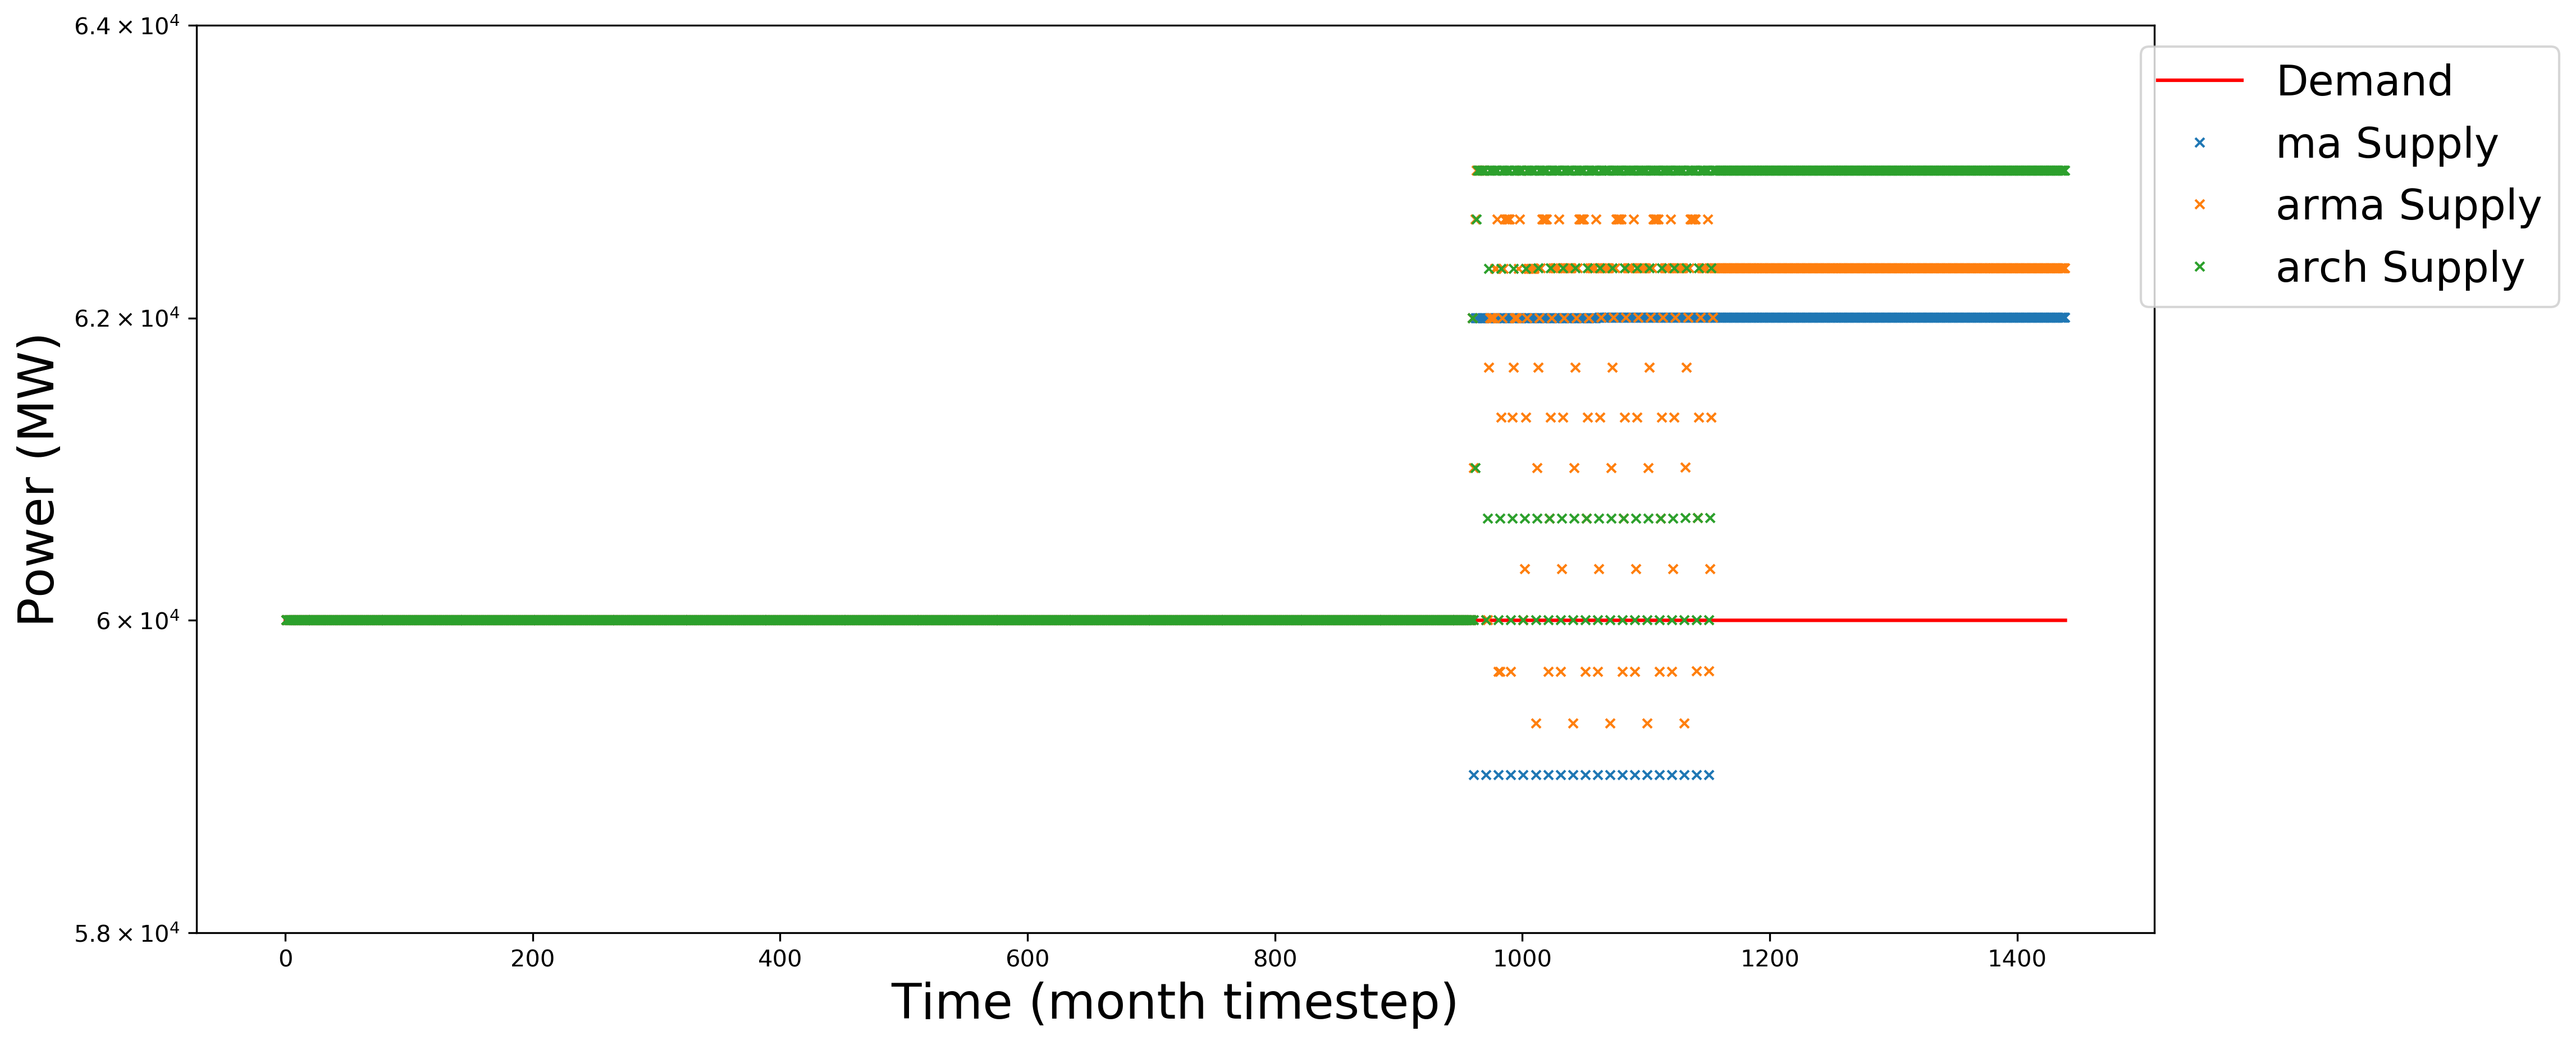
\includegraphics[width=\linewidth]{24-power-bufferB20001.png} 
		\caption{NO algorithms.}
		\label{fig:24powerNO}
	\end{subfigure}
	\vspace{1cm}
	\begin{subfigure}[t]{\textwidth}
		\centering
		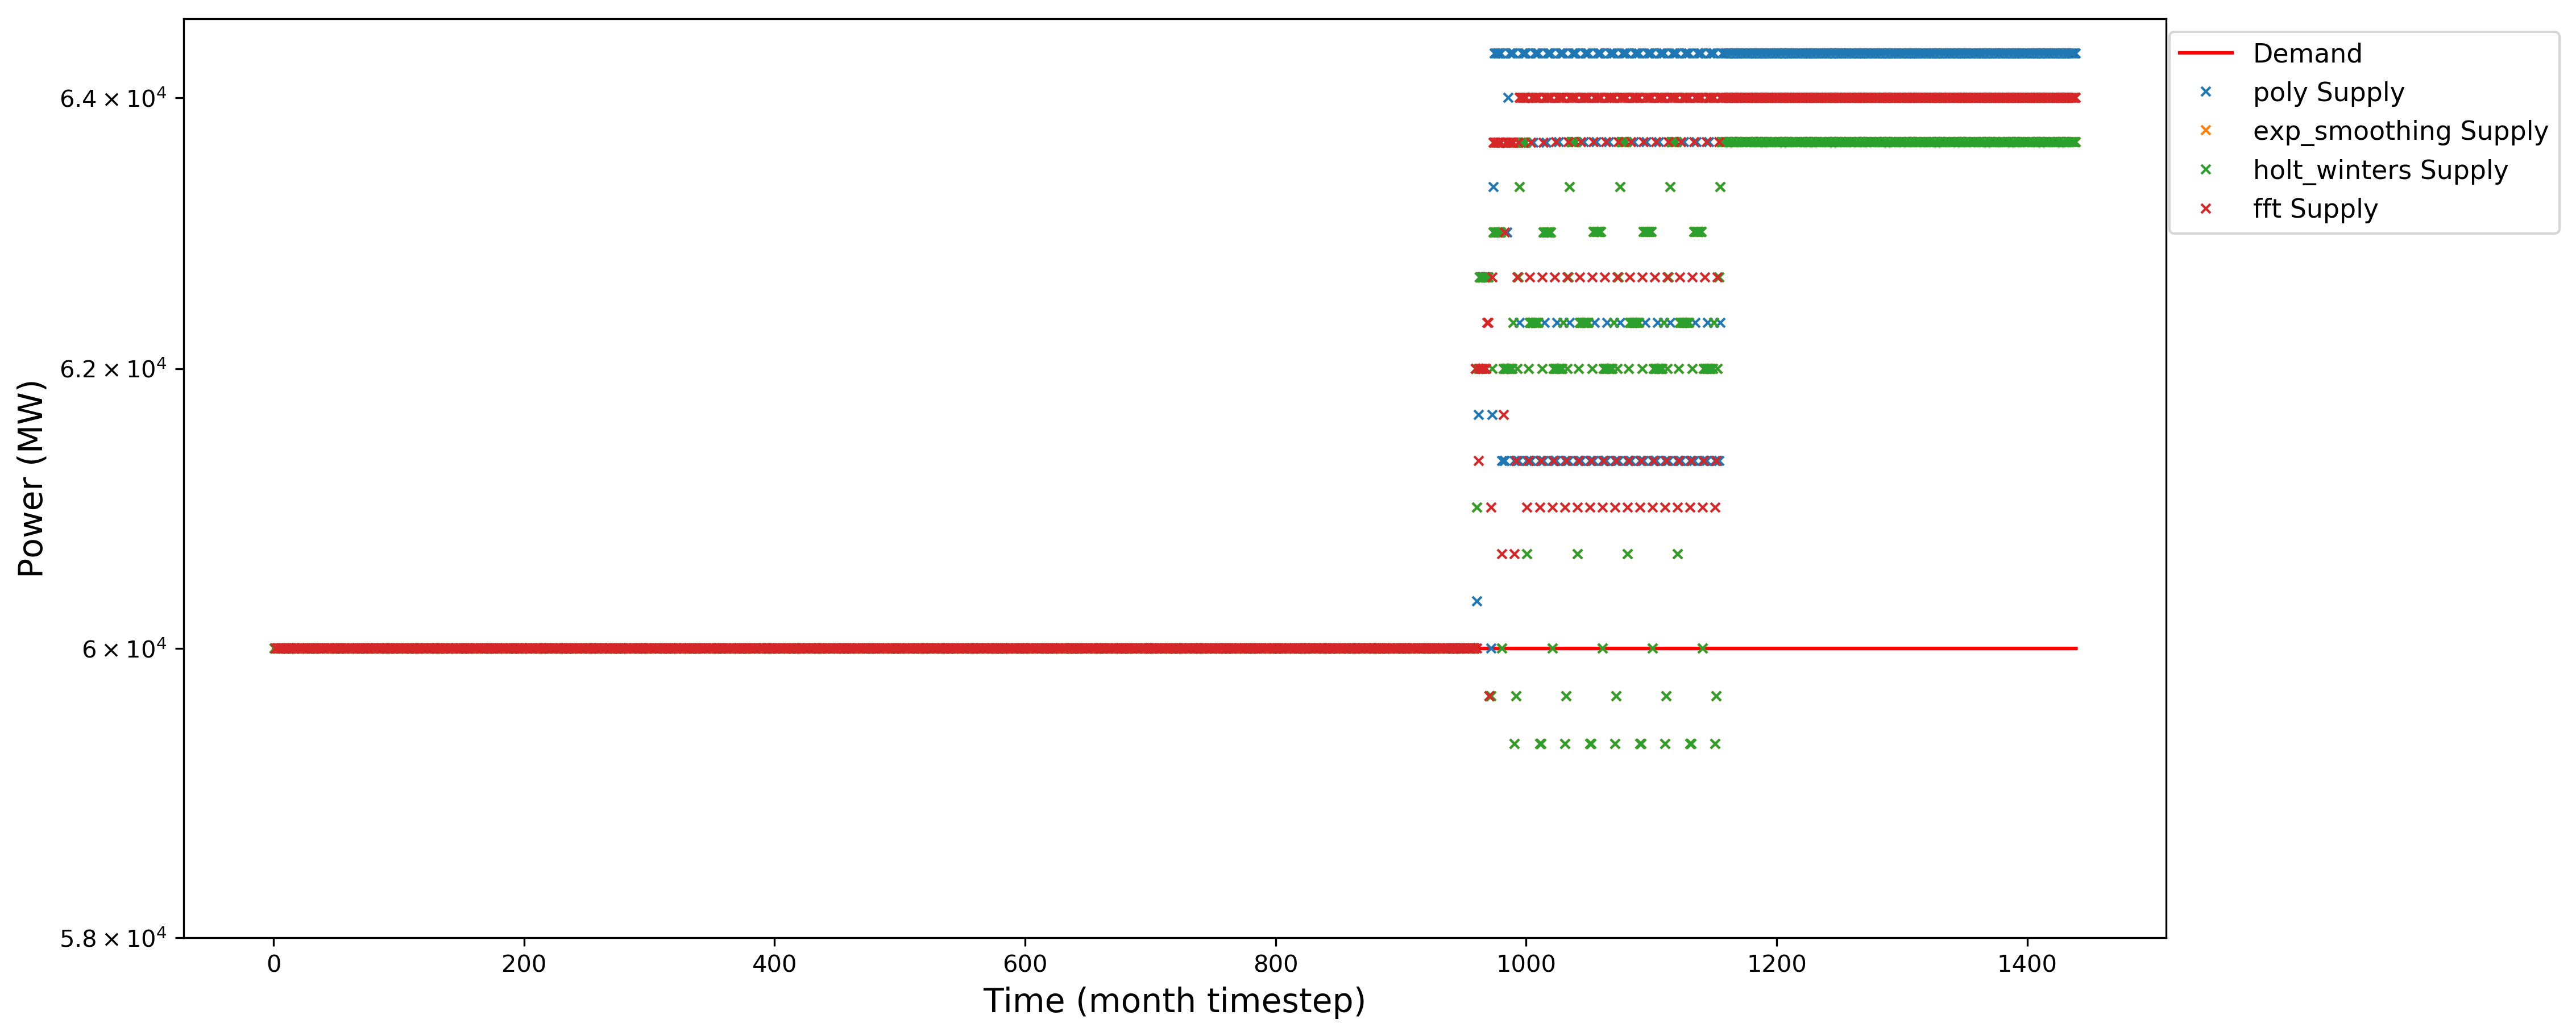
\includegraphics[width=\linewidth]{24-power-bufferB20002.png} 
		\caption{DO algorithms.}
		\label{fig:24powerDO}
	\end{subfigure}
	\begin{subfigure}[t]{.95\textwidth}
		\centering
		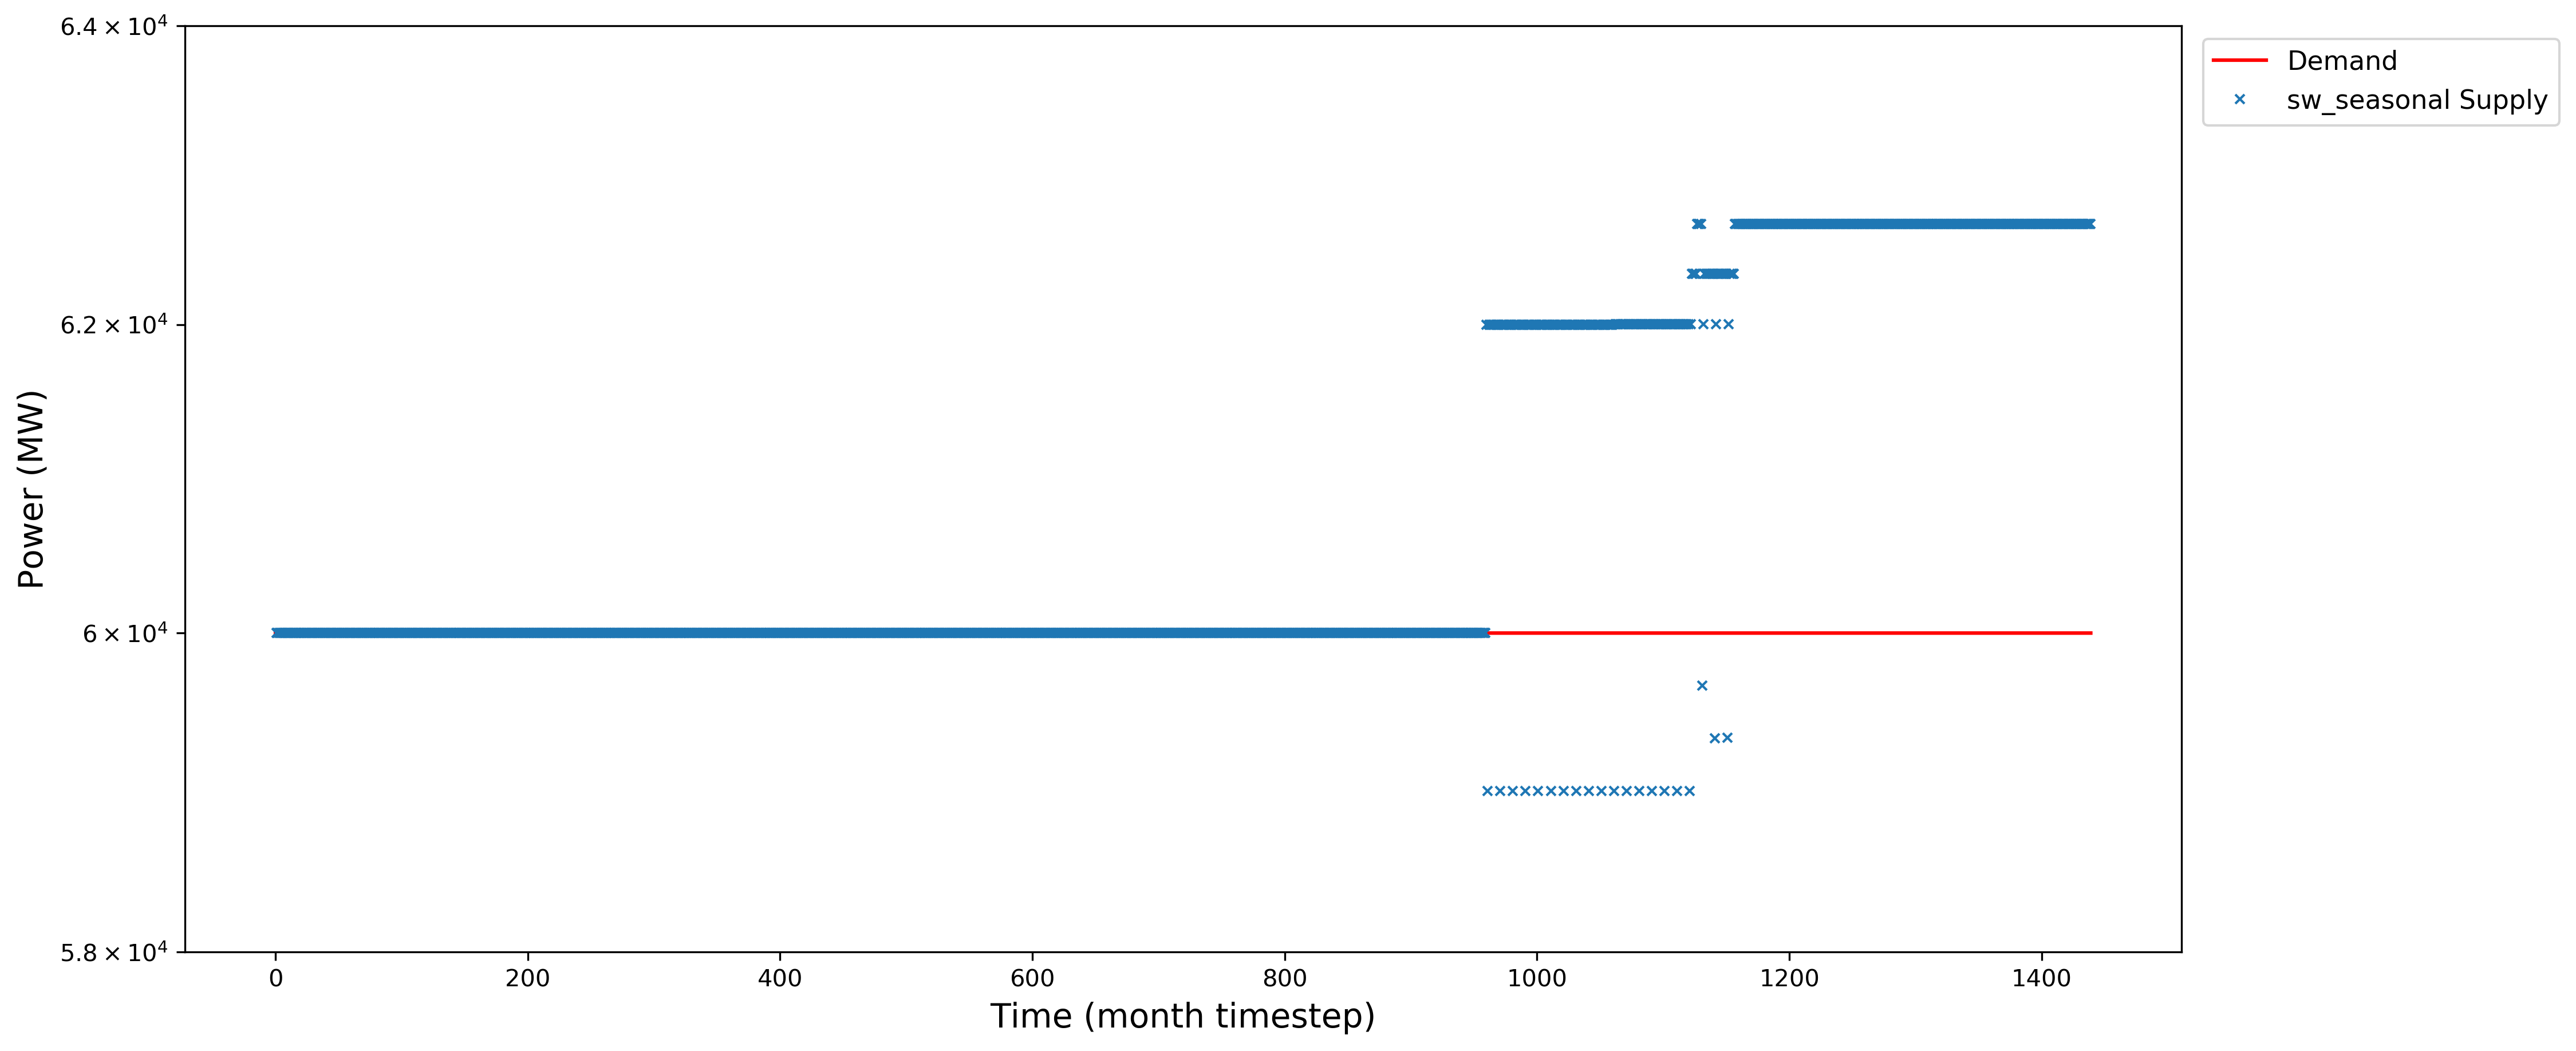
\includegraphics[width=\linewidth]{24-power-bufferB20003.png} 
		\caption{SO algorithms.}
		\label{fig:24powerSO}
\end{subfigure}
	\hfill
	\caption{Plot of the power demand and supply of EG01-EG24 for a constant power demand of 60GW for different prediction algorithms.}
	\label{fig:24power}
\end{figure*}

\subsection{Buffer Size}

This section focuses on the analysis of undersupply dependency on buffer size in the EG01-EG23 transition scenario. Table \ref{tab:buff_size} shows the number of time steps that contain undersupply and the cumulative undersupply for different buffer sizes for various prediction methods. Figure \ref{buffer_dep} displays the cumulative undersupply as a function of buffer size.

\begin{table*}[h]
	\centering
	\caption {Dependency of the undersupply of Power on the buffer size.}
	\label{tab:buff_size}
	\begin{tabular}{|l|c|c|c|c|c|c|}
	\hline
	\begin{tabular}[c]{@{}l@{}}Buffer\\ {[}MW{]}\end{tabular} & Algorithm                                                                  & MA   & ARMA & POLY & EXP\_SMOOTHING & FFT  \\ \hline
	\multirow{2}{*}{0}                          & \begin{tabular}[c]{@{}l@{}}No. of time steps\\ of undersupply\end{tabular} & 20   & 60   & 75   & 30             & 28   \\ \cline{2-7} 
	& Cumulative {[}GW{]}                                                        & 60.0 & 87.3 & 52.9 & 68.3           & 93.3 \\ \hline
	\multirow{2}{*}{2000}                       & \begin{tabular}[c]{@{}l@{}}No. of time steps\\ of undersupply\end{tabular} & 20   & 18   & 1    & 20             & 2    \\ \cline{2-7} 
	& Cumulative {[}GW{]}                                                        & 20.0 & 7.7  & 0.3  & 11.0           & 60.3 \\ \hline
	\multirow{2}{*}{4000} & \begin{tabular}[c]{@{}l@{}}No. of time steps\\ of undersupply\end{tabular} & 0    & 0    & 0    & 0              & 1    \\ \cline{2-7} 
	& Cumulative {[}GW{]}                                                        & 0    & 0    & 0    & 0              & 60.  \\ \hline
	\end{tabular}
\end{table*}

\begin{figure*}[h!]
	\centering
	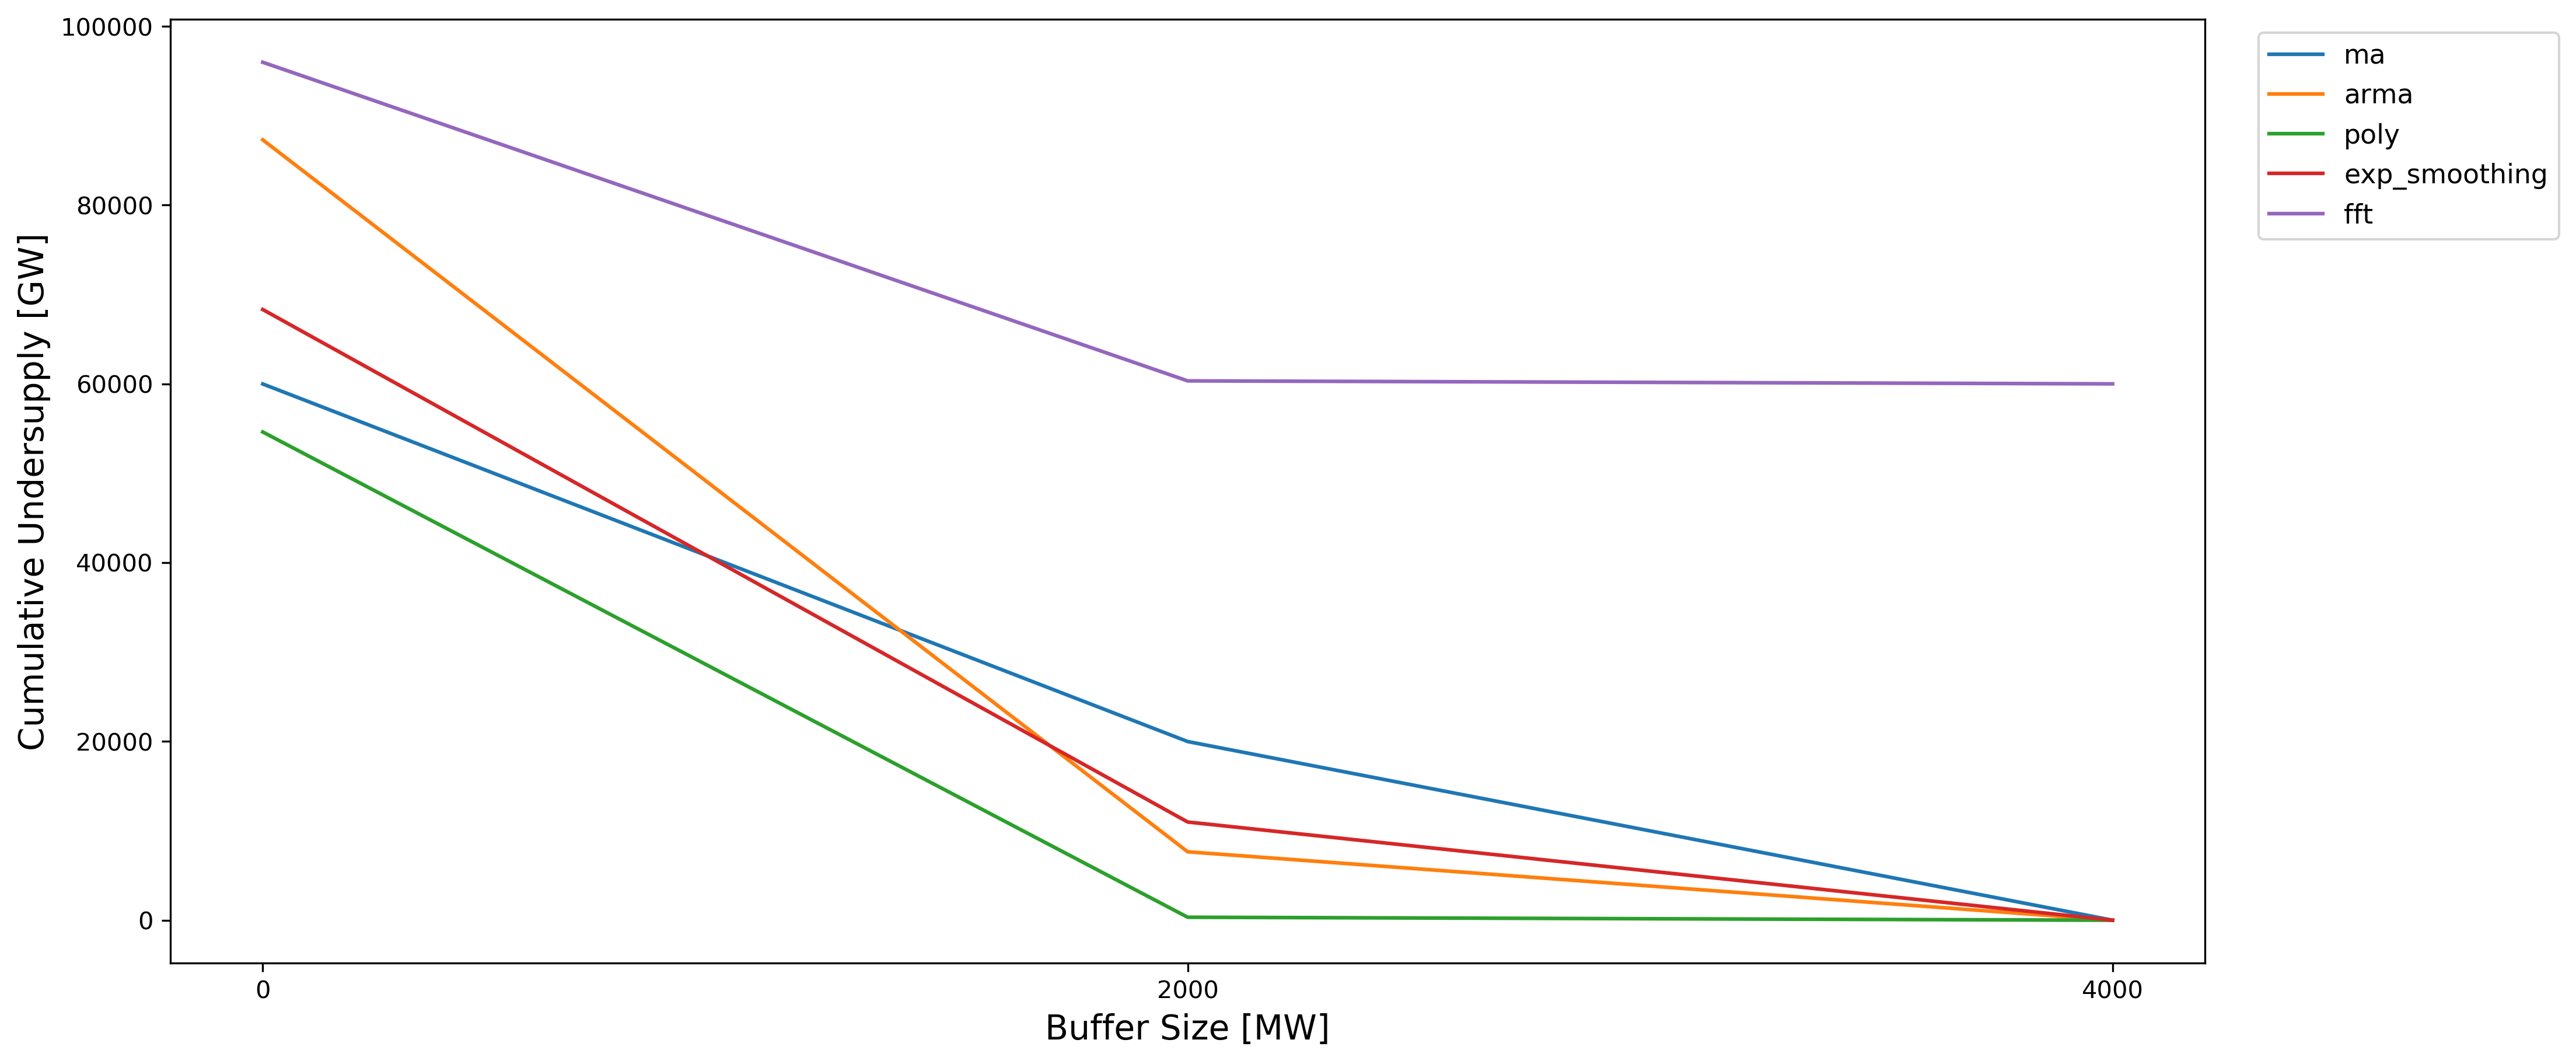
\includegraphics[width=\linewidth]{23-buff.png}
	\caption{Plot of the dependency of the undersupply of Power on the buffer size.}
	\label{buffer_dep}
\end{figure*}

\subsection{Number of Forward Steps}

This section focuses on the dependency on the number of forward steps calculated at each time step by the prediction methods in scenario EG01-EG23; the buffer size was fixed at 2000 MW. Table \ref{tab:for_steps} shows number of time steps containing undersupply and the cumulative undersupply for different forward steps for some of the prediction methods. Figure \ref{for_dep} displays the cumulative undersupply as a function of the no. of forward steps.

\begin{table*}[]
	\centering
	\caption {Dependency of the undersupply of Power on the no. of forward steps.}
	\label{tab:for_steps}
	\begin{tabular}{|l|c|c|c|c|c|c|}
		\hline
		\begin{tabular}[c]{@{}l@{}}No. of \\forward \\steps\end{tabular} & Algorithm                                                                  & MA   & ARMA & POLY & EXP\_SMOOTHING & FFT  \\ \hline
		\multirow{2}{*}{1}                          & \begin{tabular}[c]{@{}l@{}}No. of time steps\\ of undersupply\end{tabular} & 18   & 20   & 2   & 20             & 1   \\ \cline{2-7} 
		& Cumulative {[}GW{]}                                                        & 7.6 & 11.0 & 60.3 & 20.0           & 0.3 \\ \hline
		\multirow{2}{*}{3}                       & \begin{tabular}[c]{@{}l@{}}No. of time steps\\ of undersupply\end{tabular} & 1   & 20   & 2    & 0             & 1    \\ \cline{2-7} 
		& Cumulative {[}GW{]}                                                        & 0.3 & 11.0  & 60.3  & 0           & 0.3 \\ \hline
		\multirow{2}{*}{5} & \begin{tabular}[c]{@{}l@{}}No. of time steps\\ of undersupply\end{tabular} & 4    & 20    & 20    & 0              & 1    \\ \cline{2-7} 
		& Cumulative {[}GW{]}                                                        & 1.3    & 11.0    & 60.3    & 0              & 0.3  \\ \hline
	\end{tabular}
\end{table*}

\begin{figure*}[h!]
	\centering
	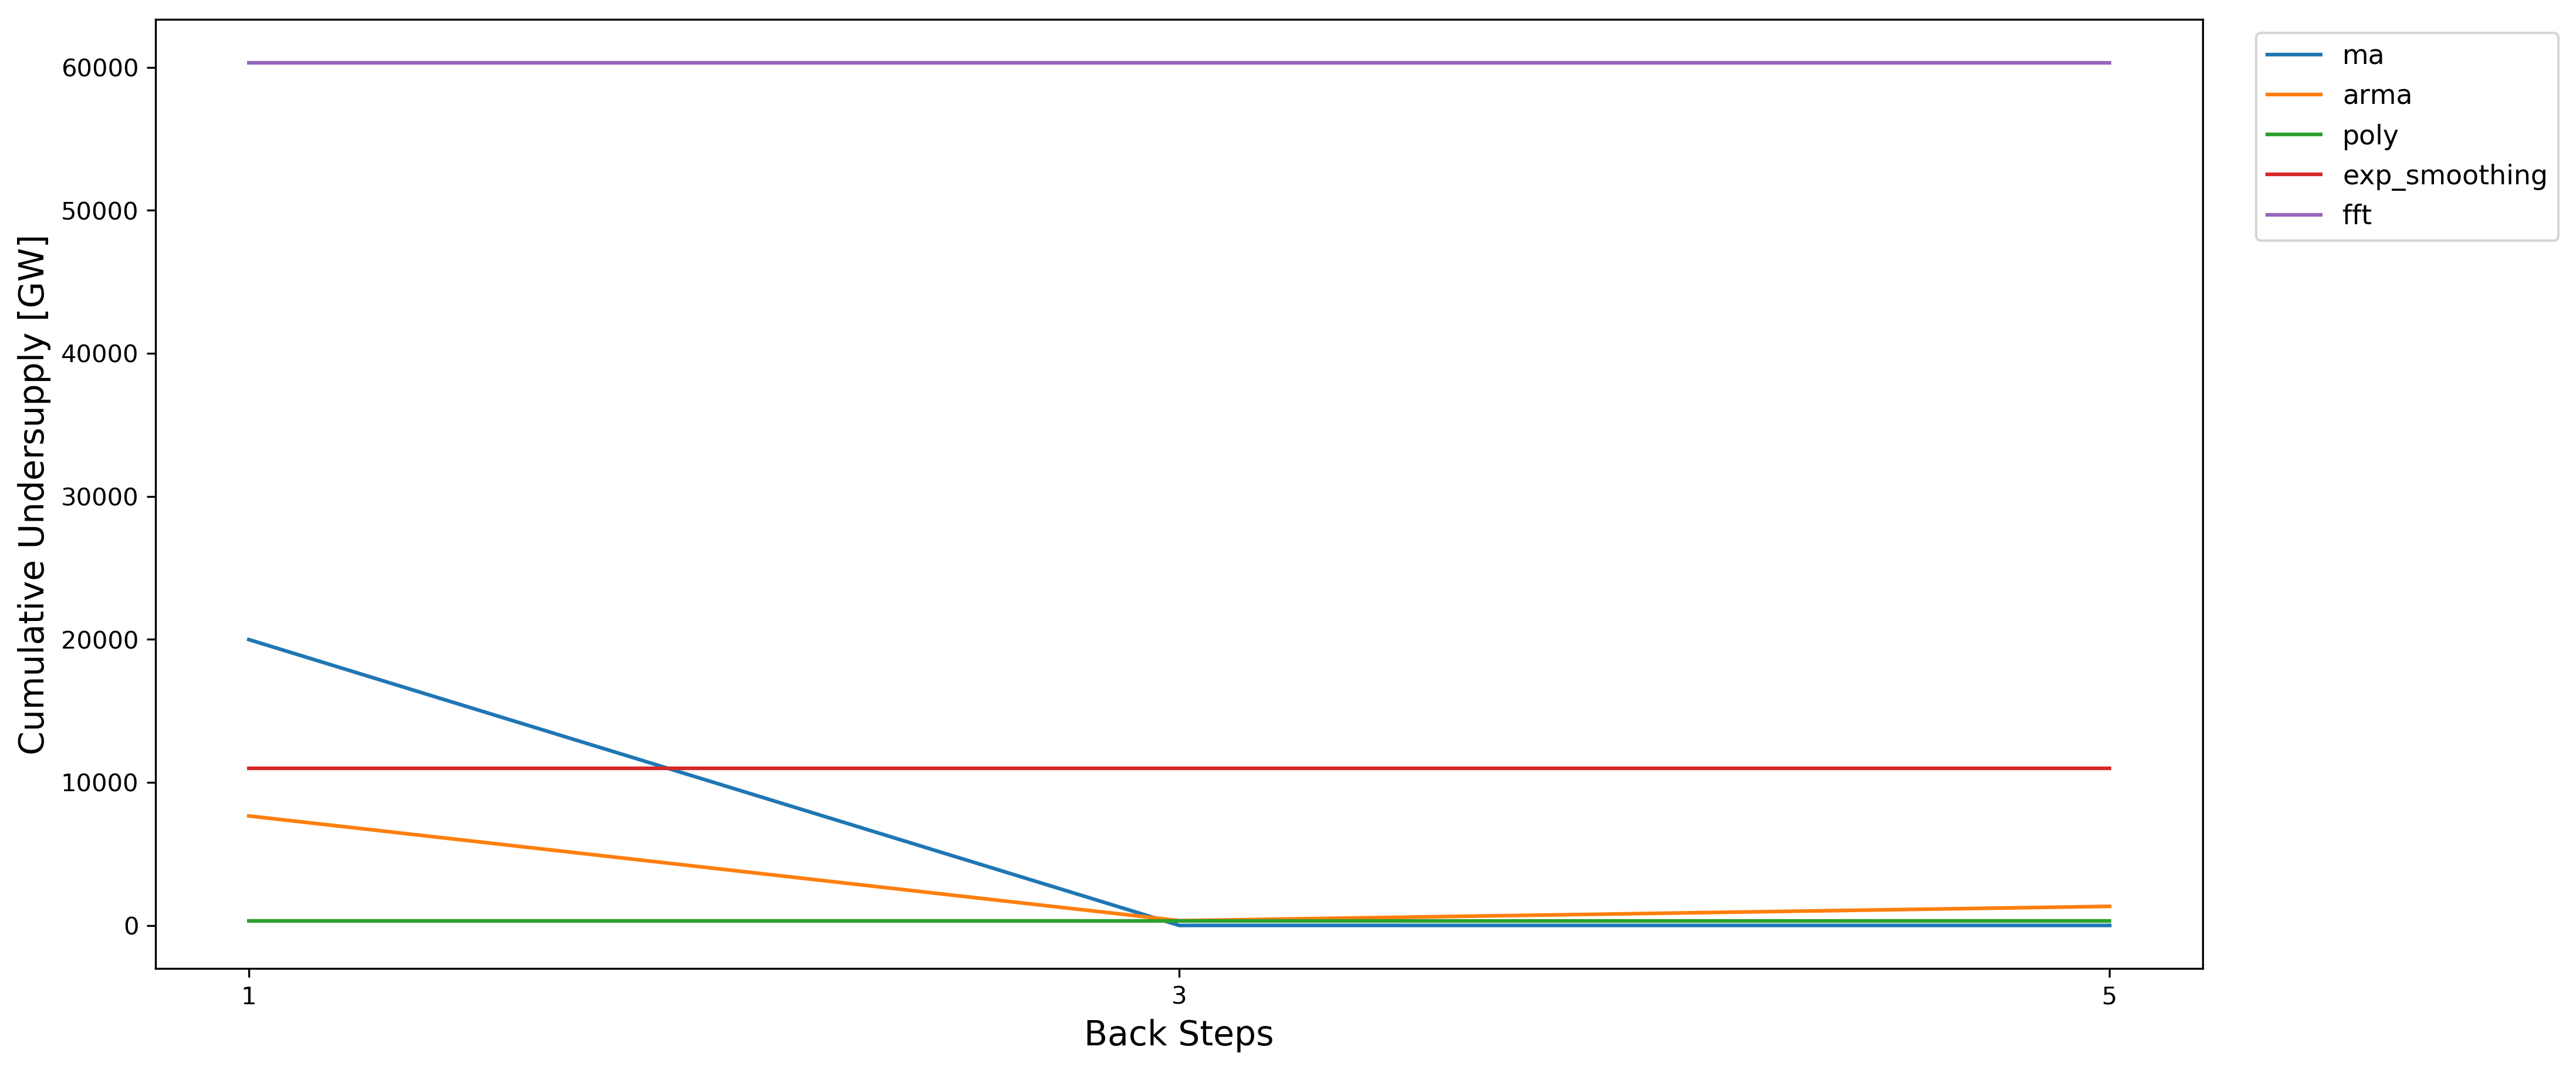
\includegraphics[width=\linewidth]{23-for.png}
	\caption{Plot of the dependency of the undersupply of Power on the no. of forward steps.}
	\label{for_dep}
\end{figure*}

\section{Conclusion and Next Steps}
This paper describes the capabilities of \deploy and demonstrates 
the use of \deploy for simple transition scenarios with 
constant, linearly increasing, and sinusoidal power demand.
The demonstration goes further with the more complex transition
scenarios EG01-EG23 and EG01-EG24. This paper also provides insights on
parameter inputs to ease the setup of larger transition scenarios
that may include numerous facilities.

Future work includes setup of similar power demand transition 
scenarios for extended nuclear fuel cycles incorporating multiple reactor designs that consequently use different types of fuel. Such cases are 
currently under study. \cite{wigeland_nuclear_2014} established the transition
scenarios EG01-EG29 and EG01-EG30. These scenarios are more complex than the
cases presented in this report and the distribution of fuel between different
reactor technologies play a main role in the transition.
Additionally, as seen during the demonstration of \deploy capabilities, a Decommissioning capability is highly useful for the setup of several NFCs and is currently under development.

\section{Acknowledgements}
This research is funded by the \gls{DOE} Office of 
Nuclear Energy's Nuclear Energy University Program (Project 16-10512) 
"Demand-Driven Cycamore Archetypes". The authors would like to thank 
members of the \gls{ARFC} group at the University of Illinois at 
Urbana-Champaign. 
We also thank our colleagues from the \Cyclus community, 
particularly those in the University of Wisconsin 
\gls{CNERG} and the University of South Carolina Energy Research 
Group (ERGS) for collaborative \Cyclus development.
%----------------------------------------------------------------%

\pagebreak 
\bibliographystyle{plain}
\bibliography{bibliography}

\end{document}


